% Options for packages loaded elsewhere
\PassOptionsToPackage{unicode}{hyperref}
\PassOptionsToPackage{hyphens}{url}
%
\documentclass[
]{book}
\usepackage{amsmath,amssymb}
\usepackage{lmodern}
\usepackage{ifxetex,ifluatex}
\ifnum 0\ifxetex 1\fi\ifluatex 1\fi=0 % if pdftex
  \usepackage[T1]{fontenc}
  \usepackage[utf8]{inputenc}
  \usepackage{textcomp} % provide euro and other symbols
\else % if luatex or xetex
  \usepackage{unicode-math}
  \defaultfontfeatures{Scale=MatchLowercase}
  \defaultfontfeatures[\rmfamily]{Ligatures=TeX,Scale=1}
\fi
% Use upquote if available, for straight quotes in verbatim environments
\IfFileExists{upquote.sty}{\usepackage{upquote}}{}
\IfFileExists{microtype.sty}{% use microtype if available
  \usepackage[]{microtype}
  \UseMicrotypeSet[protrusion]{basicmath} % disable protrusion for tt fonts
}{}
\makeatletter
\@ifundefined{KOMAClassName}{% if non-KOMA class
  \IfFileExists{parskip.sty}{%
    \usepackage{parskip}
  }{% else
    \setlength{\parindent}{0pt}
    \setlength{\parskip}{6pt plus 2pt minus 1pt}}
}{% if KOMA class
  \KOMAoptions{parskip=half}}
\makeatother
\usepackage{xcolor}
\IfFileExists{xurl.sty}{\usepackage{xurl}}{} % add URL line breaks if available
\IfFileExists{bookmark.sty}{\usepackage{bookmark}}{\usepackage{hyperref}}
\hypersetup{
  pdftitle={From Forests to Heritage: book of abstracts},
  pdfauthor={Kristof Haneca; Aoife Daly; Marta Domínguez-Delmás},
  hidelinks,
  pdfcreator={LaTeX via pandoc}}
\urlstyle{same} % disable monospaced font for URLs
\usepackage{longtable,booktabs,array}
\usepackage{calc} % for calculating minipage widths
% Correct order of tables after \paragraph or \subparagraph
\usepackage{etoolbox}
\makeatletter
\patchcmd\longtable{\par}{\if@noskipsec\mbox{}\fi\par}{}{}
\makeatother
% Allow footnotes in longtable head/foot
\IfFileExists{footnotehyper.sty}{\usepackage{footnotehyper}}{\usepackage{footnote}}
\makesavenoteenv{longtable}
\usepackage{graphicx}
\makeatletter
\def\maxwidth{\ifdim\Gin@nat@width>\linewidth\linewidth\else\Gin@nat@width\fi}
\def\maxheight{\ifdim\Gin@nat@height>\textheight\textheight\else\Gin@nat@height\fi}
\makeatother
% Scale images if necessary, so that they will not overflow the page
% margins by default, and it is still possible to overwrite the defaults
% using explicit options in \includegraphics[width, height, ...]{}
\setkeys{Gin}{width=\maxwidth,height=\maxheight,keepaspectratio}
% Set default figure placement to htbp
\makeatletter
\def\fps@figure{htbp}
\makeatother
\setlength{\emergencystretch}{3em} % prevent overfull lines
\providecommand{\tightlist}{%
  \setlength{\itemsep}{0pt}\setlength{\parskip}{0pt}}
\setcounter{secnumdepth}{5}
\usepackage{booktabs}
\renewcommand{\contentsname}{}
\usepackage{booktabs}
\usepackage{longtable}
\usepackage{array}
\usepackage{multirow}
\usepackage{wrapfig}
\usepackage{float}
\usepackage{colortbl}
\usepackage{pdflscape}
\usepackage{tabu}
\usepackage{threeparttable}
\usepackage{threeparttablex}
\usepackage[normalem]{ulem}
\usepackage{makecell}
\usepackage{xcolor}
\ifluatex
  \usepackage{selnolig}  % disable illegal ligatures
\fi
\usepackage[]{natbib}
\bibliographystyle{plainnat}

\title{From Forests to Heritage: book of abstracts}
\author{Kristof Haneca \and Aoife Daly \and Marta Domínguez-Delmás}
\date{18 februari, 2022}

\begin{document}
\maketitle

{
\setcounter{tocdepth}{1}
\tableofcontents
}
\hypertarget{book-of-abstracts}{%
\chapter*{Book of abstracts}\label{book-of-abstracts}}
\addcontentsline{toc}{chapter}{Book of abstracts}

Conference website: \url{https://www.forests2heritage.nl/}

\href{https://event.forests2heritage.nl/}{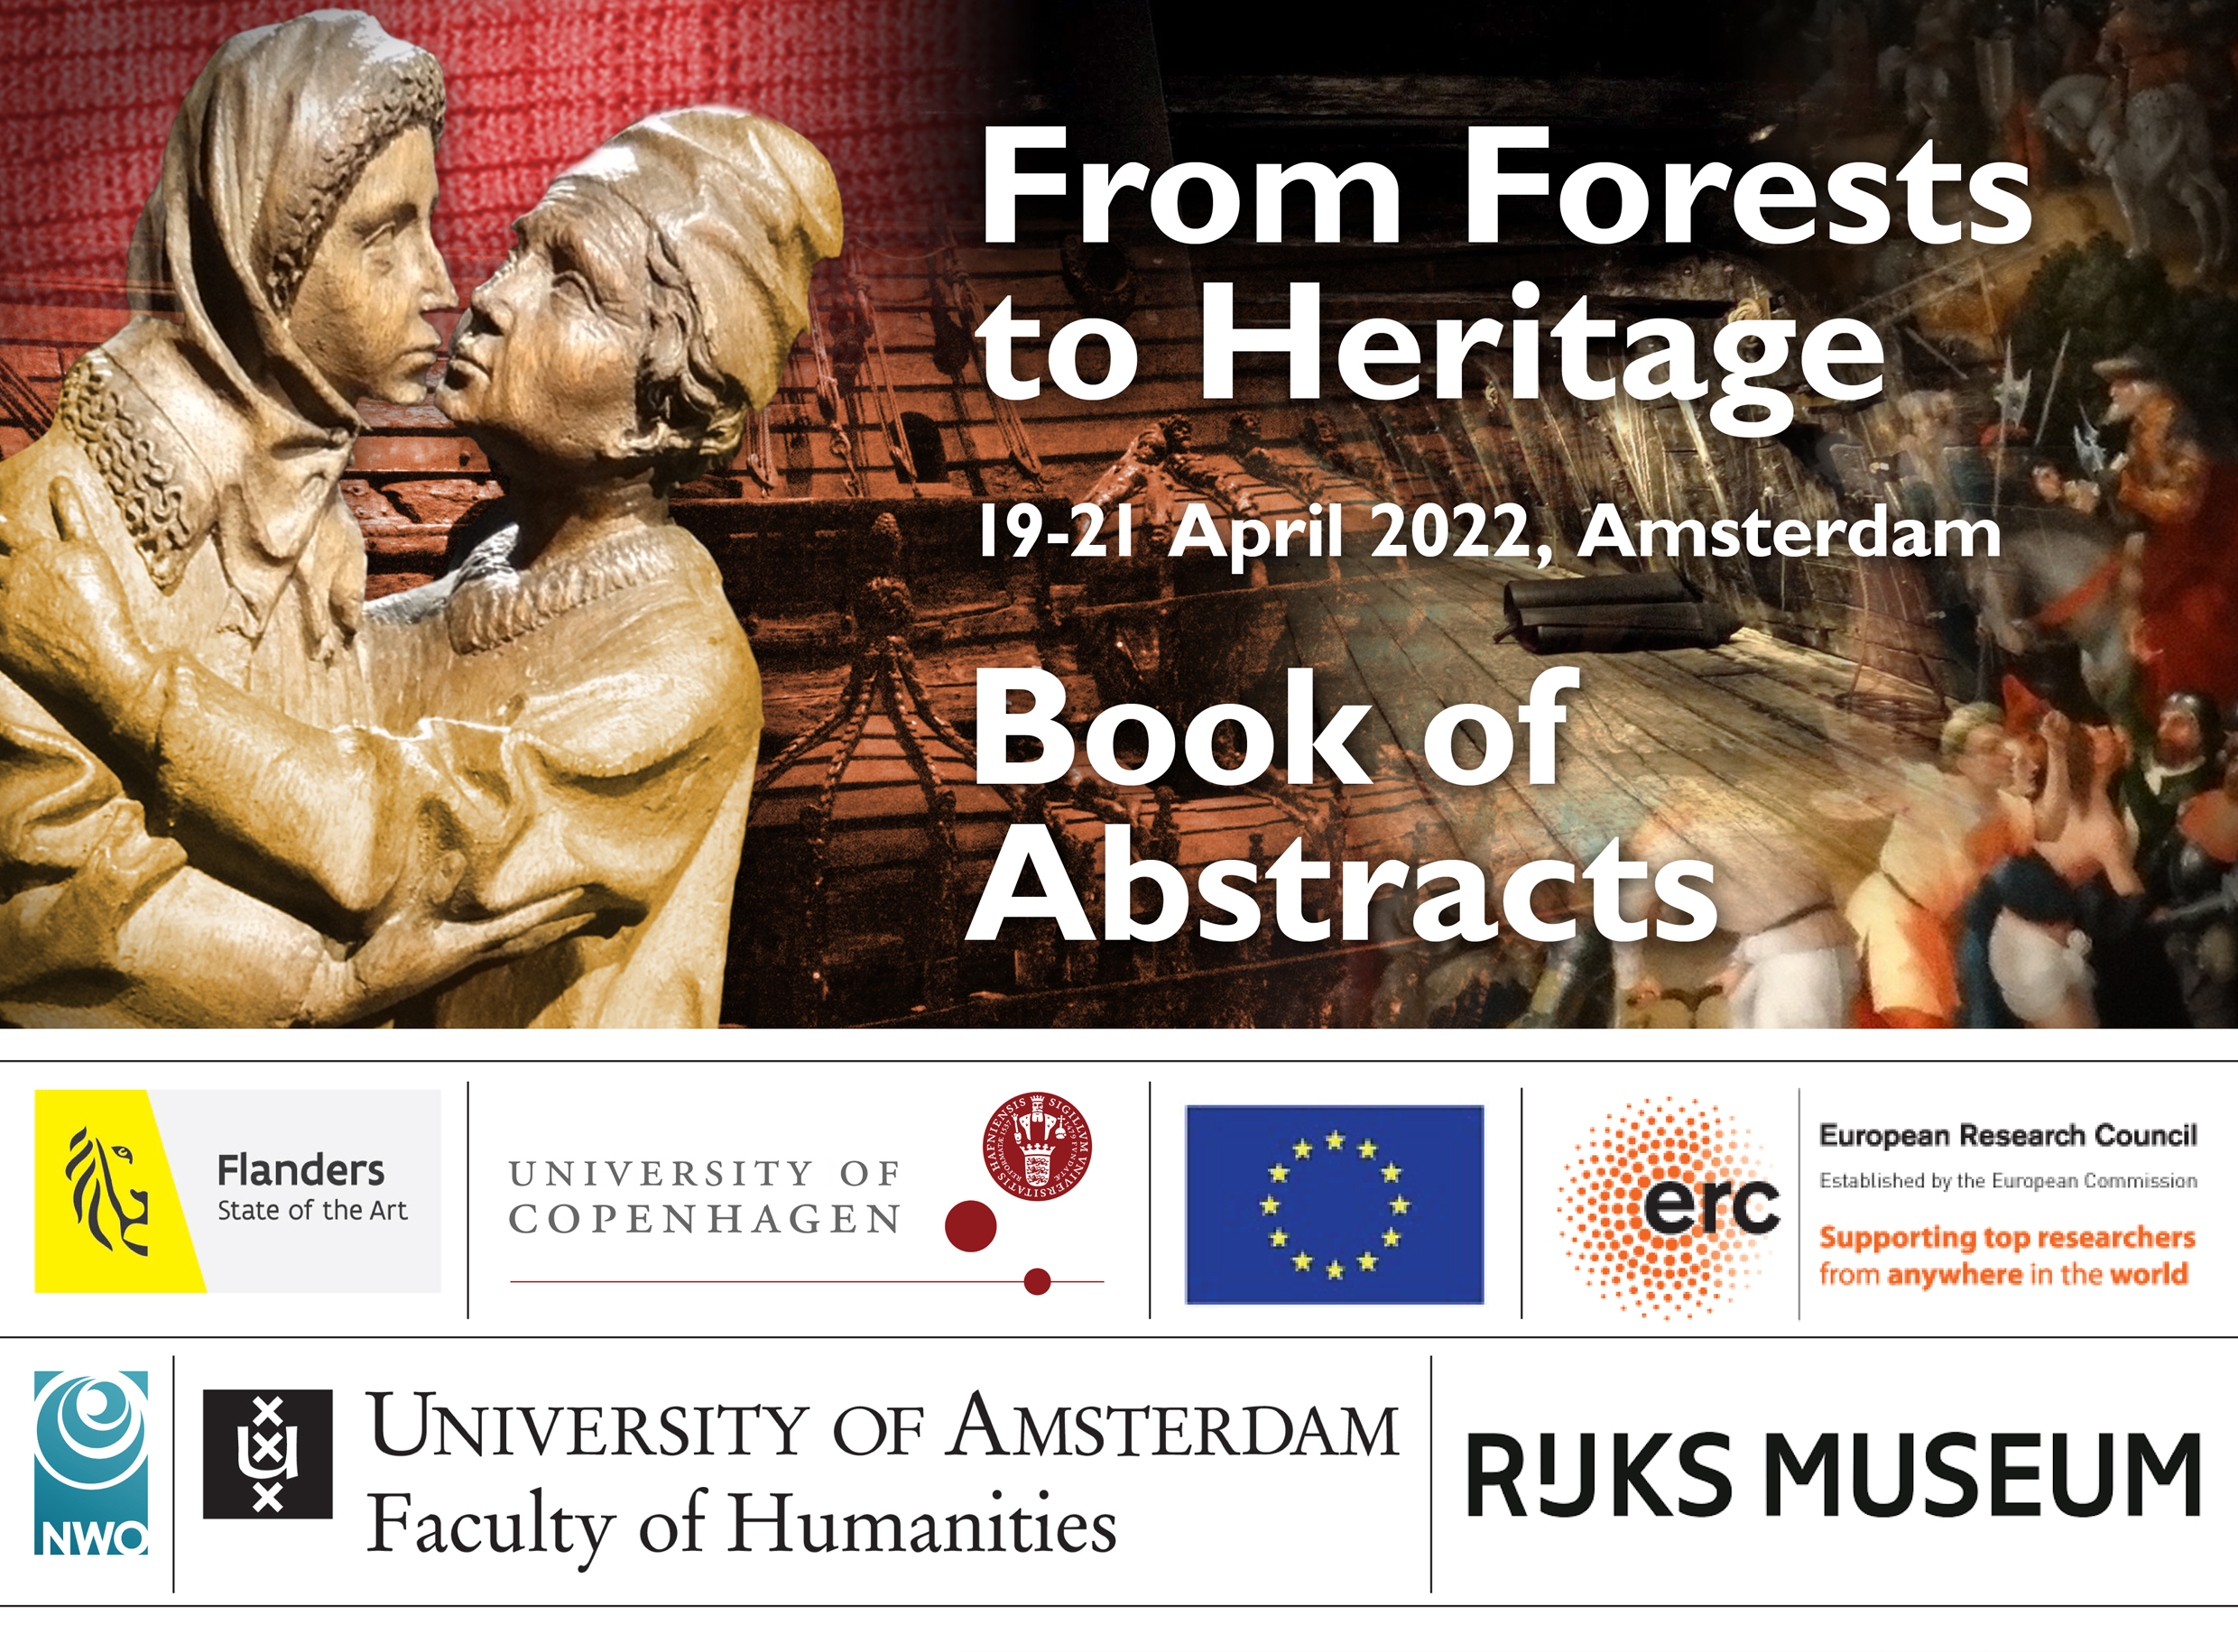
\includegraphics[width=1\textwidth,height=\textheight]{bookofAbstracts header.jpg}}

\hypertarget{part-program}{%
\part*{PROGRAM}\label{part-program}}
\addcontentsline{toc}{part}{PROGRAM}

\hypertarget{program}{%
\chapter*{Program}\label{program}}
\addcontentsline{toc}{chapter}{Program}

\hypertarget{monday-18-april-2022}{%
\section*{Monday: 18 April 2022}\label{monday-18-april-2022}}
\addcontentsline{toc}{section}{Monday: 18 April 2022}

\begin{verbatim}
#> Warning in latex_new_row_builder(target_row, table_info,
#> bold, italic, monospace, : Setting full_width = TRUE will
#> turn the table into a tabu environment where colors are not
#> really easily configable with this package. Please consider
#> turn off full_width.
\end{verbatim}

\begin{tabu} to \linewidth {>{\raggedright}X>{\raggedright}X>{\raggedright}X>{\raggedright}X>{\raggedright}X}
\hline
timing & event & presenter & title & session\\
\hline
\cellcolor[HTML]{D6EAF8}{18:00 - 20:00} & \cellcolor[HTML]{D6EAF8}{Registration and icebreaker} & \cellcolor[HTML]{D6EAF8}{} & \cellcolor[HTML]{D6EAF8}{} & \cellcolor[HTML]{D6EAF8}{}\\
\hline
\end{tabu}

\hypertarget{tuesday-19-april-2022}{%
\section*{Tuesday: 19 April 2022}\label{tuesday-19-april-2022}}
\addcontentsline{toc}{section}{Tuesday: 19 April 2022}

\begin{verbatim}
#> Warning in latex_new_row_builder(target_row, table_info,
#> bold, italic, monospace, : Setting full_width = TRUE will
#> turn the table into a tabu environment where colors are not
#> really easily configable with this package. Please consider
#> turn off full_width.

#> Warning in latex_new_row_builder(target_row, table_info,
#> bold, italic, monospace, : Setting full_width = TRUE will
#> turn the table into a tabu environment where colors are not
#> really easily configable with this package. Please consider
#> turn off full_width.

#> Warning in latex_new_row_builder(target_row, table_info,
#> bold, italic, monospace, : Setting full_width = TRUE will
#> turn the table into a tabu environment where colors are not
#> really easily configable with this package. Please consider
#> turn off full_width.

#> Warning in latex_new_row_builder(target_row, table_info,
#> bold, italic, monospace, : Setting full_width = TRUE will
#> turn the table into a tabu environment where colors are not
#> really easily configable with this package. Please consider
#> turn off full_width.

#> Warning in latex_new_row_builder(target_row, table_info,
#> bold, italic, monospace, : Setting full_width = TRUE will
#> turn the table into a tabu environment where colors are not
#> really easily configable with this package. Please consider
#> turn off full_width.

#> Warning in latex_new_row_builder(target_row, table_info,
#> bold, italic, monospace, : Setting full_width = TRUE will
#> turn the table into a tabu environment where colors are not
#> really easily configable with this package. Please consider
#> turn off full_width.

#> Warning in latex_new_row_builder(target_row, table_info,
#> bold, italic, monospace, : Setting full_width = TRUE will
#> turn the table into a tabu environment where colors are not
#> really easily configable with this package. Please consider
#> turn off full_width.

#> Warning in latex_new_row_builder(target_row, table_info,
#> bold, italic, monospace, : Setting full_width = TRUE will
#> turn the table into a tabu environment where colors are not
#> really easily configable with this package. Please consider
#> turn off full_width.

#> Warning in latex_new_row_builder(target_row, table_info,
#> bold, italic, monospace, : Setting full_width = TRUE will
#> turn the table into a tabu environment where colors are not
#> really easily configable with this package. Please consider
#> turn off full_width.

#> Warning in latex_new_row_builder(target_row, table_info,
#> bold, italic, monospace, : Setting full_width = TRUE will
#> turn the table into a tabu environment where colors are not
#> really easily configable with this package. Please consider
#> turn off full_width.

#> Warning in latex_new_row_builder(target_row, table_info,
#> bold, italic, monospace, : Setting full_width = TRUE will
#> turn the table into a tabu environment where colors are not
#> really easily configable with this package. Please consider
#> turn off full_width.

#> Warning in latex_new_row_builder(target_row, table_info,
#> bold, italic, monospace, : Setting full_width = TRUE will
#> turn the table into a tabu environment where colors are not
#> really easily configable with this package. Please consider
#> turn off full_width.

#> Warning in latex_new_row_builder(target_row, table_info,
#> bold, italic, monospace, : Setting full_width = TRUE will
#> turn the table into a tabu environment where colors are not
#> really easily configable with this package. Please consider
#> turn off full_width.

#> Warning in latex_new_row_builder(target_row, table_info,
#> bold, italic, monospace, : Setting full_width = TRUE will
#> turn the table into a tabu environment where colors are not
#> really easily configable with this package. Please consider
#> turn off full_width.

#> Warning in latex_new_row_builder(target_row, table_info,
#> bold, italic, monospace, : Setting full_width = TRUE will
#> turn the table into a tabu environment where colors are not
#> really easily configable with this package. Please consider
#> turn off full_width.

#> Warning in latex_new_row_builder(target_row, table_info,
#> bold, italic, monospace, : Setting full_width = TRUE will
#> turn the table into a tabu environment where colors are not
#> really easily configable with this package. Please consider
#> turn off full_width.

#> Warning in latex_new_row_builder(target_row, table_info,
#> bold, italic, monospace, : Setting full_width = TRUE will
#> turn the table into a tabu environment where colors are not
#> really easily configable with this package. Please consider
#> turn off full_width.

#> Warning in latex_new_row_builder(target_row, table_info,
#> bold, italic, monospace, : Setting full_width = TRUE will
#> turn the table into a tabu environment where colors are not
#> really easily configable with this package. Please consider
#> turn off full_width.

#> Warning in latex_new_row_builder(target_row, table_info,
#> bold, italic, monospace, : Setting full_width = TRUE will
#> turn the table into a tabu environment where colors are not
#> really easily configable with this package. Please consider
#> turn off full_width.

#> Warning in latex_new_row_builder(target_row, table_info,
#> bold, italic, monospace, : Setting full_width = TRUE will
#> turn the table into a tabu environment where colors are not
#> really easily configable with this package. Please consider
#> turn off full_width.
\end{verbatim}

\begin{tabu} to \linewidth {>{\raggedright}X>{\raggedright}X>{\raggedright}X>{\raggedright}X>{\raggedright}X}
\hline
timing & event & presenter & title & session\\
\hline
\cellcolor[HTML]{D6EAF8}{8:30 - 9:00} & \cellcolor[HTML]{D6EAF8}{Registration} & \cellcolor[HTML]{D6EAF8}{} & \cellcolor[HTML]{D6EAF8}{} & \cellcolor[HTML]{D6EAF8}{}\\
\hline
\cellcolor[HTML]{D6EAF8}{9:00 - 9:30} & \cellcolor[HTML]{D6EAF8}{kickoff} & \cellcolor[HTML]{D6EAF8}{Marta, Aoife \& Kristof} & \cellcolor[HTML]{D6EAF8}{} & \cellcolor[HTML]{D6EAF8}{}\\
\hline
\cellcolor[HTML]{D6EAF8}{9:30 - 12:30} & \cellcolor[HTML]{D6EAF8}{session 1 \& 2} & \cellcolor[HTML]{D6EAF8}{} & \cellcolor[HTML]{D6EAF8}{} & \cellcolor[HTML]{D6EAF8}{}\\
\hline
9:30 - 9:45 & [S1-O-001](\#s1-o-001) & Elie Pinta & Exploring the significance, acquisition and use of wooden resources between Norse Greenland and North America: a (re)examination of literary and archaeological sources & 1. Forest history\\
\hline
9:45 - 10:00 & [S1-O-002](\#s1-o-002) & Anna Helena Petersén & Reconstruction of economic resources associated with timber building architecture in early medieval urban Trondheim & 1. Forest history\\
\hline
10:00 - 10:15 & [S1-O-003](\#s1-o-003) & Linar Akhmetzyanov & A dendroecological reconstruction of forest management history in Mediterranean Abies pinsapo forests & 1. Forest history\\
\hline
10:15 - 10:30 & [S1-O-004](\#s1-o-004) & Sabrina Bianco & Wood for funerary pyres in Barcino (Barcelona, NE Iberian Peninsula): investigating cremation structures in two necropolis (1st-3rd centuries CE) starting from charcoal analysis & 1. Forest history\\
\hline
\cellcolor[HTML]{D6EAF8}{10:30 - 10:35} & \cellcolor[HTML]{D6EAF8}{posters} & \cellcolor[HTML]{D6EAF8}{} & \cellcolor[HTML]{D6EAF8}{one-minute poster pitches} & \cellcolor[HTML]{D6EAF8}{1. Forest history posters (4)}\\
\hline
\cellcolor[HTML]{F2F2F2}{} & \cellcolor[HTML]{F2F2F2}{[S1-P-001](\#s1-p-001)} & \cellcolor[HTML]{F2F2F2}{Pascoal Gota} & \cellcolor[HTML]{F2F2F2}{Our history does not exist in the books: forest patches framing new identities for heritage and environmental conservation} & \cellcolor[HTML]{F2F2F2}{1. Forest history}\\
\hline
\cellcolor[HTML]{F2F2F2}{} & \cellcolor[HTML]{F2F2F2}{[S1-P-002](\#s1-p-002)} & \cellcolor[HTML]{F2F2F2}{Andreas Rais} & \cellcolor[HTML]{F2F2F2}{Mechanical wood properties over the past 100 years} & \cellcolor[HTML]{F2F2F2}{1. Forest history}\\
\hline
\cellcolor[HTML]{F2F2F2}{} & \cellcolor[HTML]{F2F2F2}{[S1-P-003](\#s1-p-003)} & \cellcolor[HTML]{F2F2F2}{Sveva Longo} & \cellcolor[HTML]{F2F2F2}{Dendrochronological investigation of monumental trees from “Villa Medicea di Castello” in Florence, Italy} & \cellcolor[HTML]{F2F2F2}{1. Forest history}\\
\hline
\cellcolor[HTML]{F2F2F2}{} & \cellcolor[HTML]{F2F2F2}{[S1-P-004](\#s1-p-004)} & \cellcolor[HTML]{F2F2F2}{Caroline Vermeeren1} & \cellcolor[HTML]{F2F2F2}{History of woodland management: the Neolithic } & \cellcolor[HTML]{F2F2F2}{1. Forest history}\\
\hline
\cellcolor[HTML]{D6EAF8}{10:35 - 11:00} & \cellcolor[HTML]{D6EAF8}{coffee} & \cellcolor[HTML]{D6EAF8}{} & \cellcolor[HTML]{D6EAF8}{} & \cellcolor[HTML]{D6EAF8}{}\\
\hline
11:00 - 11:15 & [S1-O-005](\#s1-o-005) & María Martín-Seijo & Woody resources and their management during Iron Age in northwest Iberia & 1. Forest history\\
\hline
11:15 - 11:30 & [S1-O-006](\#s1-o-006) & Oriol López-Bultó & Sorting the trees: new evidences of woodland management at La Draga (Banyoles, Spain) & 1. Forest history\\
\hline
11:30 - 11:45 & [S1-O-007](\#s1-o-007) & Lisa Shindo & From the exhaustive study of a mountain village to the restitution of forest: how far can dendrochronology go? & 1. Forest history\\
\hline
11:45 - 12:00 & [S2-O-002](\#s2-o-002) & Andrine Nilsen & Piers, wharfs and shipping at Masthugget, Gothenburg – Investigating private harbours through wood and stone structures & 2. Shipwrecks and archaeological structures\\
\hline
12:00 - 12:15 & [S2-O-003](\#s2-o-003) & Anne Crone & Marking time in the Iron Age; the dendrochronology of loch (lake) settlement in SW Scotland & 2. Shipwrecks and archaeological structures\\
\hline
12:15 - 12:30 & [S2-O-004](\#s2-o-004) & Mike Belasus & Just bad quality? Some thoughts on the use of timber in medieval to modern shipbuilding & 2. Shipwrecks and archaeological structures\\
\hline
\cellcolor[HTML]{D6EAF8}{12:30 - 13:30} & \cellcolor[HTML]{D6EAF8}{lunch} & \cellcolor[HTML]{D6EAF8}{} & \cellcolor[HTML]{D6EAF8}{} & \cellcolor[HTML]{D6EAF8}{}\\
\hline
\cellcolor[HTML]{D6EAF8}{13:30 - 15:05} & \cellcolor[HTML]{D6EAF8}{pre-recorded talks} & \cellcolor[HTML]{D6EAF8}{} & \cellcolor[HTML]{D6EAF8}{} & \cellcolor[HTML]{D6EAF8}{}\\
\hline
13:30 - 13:45 & [S2-O-001](\#s2-o-001) & Ignacio A. Mundo & Wood identification and dendrochronological techniques applied for the study of shipwrecks on the Atlantic coast of Argentina: comparison of different case studies showing limitations and potentials & 2. Shipwrecks and archaeological structures PRERECORDED\\
\hline
13:45 - 14:00 & [S4-O-001](\#s4-o-001) & Sebastian Nemestothy & Roof constructions in Austria – an overview & 4. Built heritage PRERECORDED\\
\hline
14:00 - 14:15 & [S4-O-002](\#s4-o-002) & Motonari Ohyama & A 2ka-long tree-ring chronology for hinoki cypress from central Japan and its dendroarchaeological application & 4. Built heritage PRERECORDED\\
\hline
14:15 - 14:30 & [S5-O-001](\#s5-o-001) & Michael Grabner & Short distance log transport in Austria & 5. Evidence of timber trade and transport PRERECORDED\\
\hline
14:30 - 14:45 & [S6-O-001](\#s6-o-001) & Gretel Boswijk & Isotope dendrochronology in New Zealand & 6. Novel methods for dating and provenance analysis PRERECORDED\\
\hline
14:45 - 15:00 & [S6-O-002](\#s6-o-002) & Fusa Miyake & Solar bursts recorded in tree rings & 6. Novel methods for dating and provenance analysis PRERECORDED\\
\hline
\cellcolor[HTML]{D6EAF8}{15:00 - 15:05} & \cellcolor[HTML]{D6EAF8}{posters} & \cellcolor[HTML]{D6EAF8}{} & \cellcolor[HTML]{D6EAF8}{one-minute poster pitches} & \cellcolor[HTML]{D6EAF8}{2. Shipwrecks and archaeological structures posters (5)}\\
\hline
\cellcolor[HTML]{F2F2F2}{} & \cellcolor[HTML]{F2F2F2}{[S2-P-001](\#s2-p-001)} & \cellcolor[HTML]{F2F2F2}{Abdelmoniem M. Abdelmoniem} & \cellcolor[HTML]{F2F2F2}{Conservation processes of a painted wooden coffin at Saqqara area} & \cellcolor[HTML]{F2F2F2}{2. Shipwrecks and archaeological structures}\\
\hline
\cellcolor[HTML]{F2F2F2}{} & \cellcolor[HTML]{F2F2F2}{[S2-P-002](\#s2-p-002)} & \cellcolor[HTML]{F2F2F2}{Angela Balzano} & \cellcolor[HTML]{F2F2F2}{Microscopy techniques for the examination of waterlogged archaeological wood} & \cellcolor[HTML]{F2F2F2}{2. Shipwrecks and archaeological structures}\\
\hline
\cellcolor[HTML]{F2F2F2}{} & \cellcolor[HTML]{F2F2F2}{[S2-P-003](\#s2-p-003)} & \cellcolor[HTML]{F2F2F2}{Daniel Peter Dalicsek} & \cellcolor[HTML]{F2F2F2}{Practices of shipwreck timber sampling for dendrochronology} & \cellcolor[HTML]{F2F2F2}{2. Shipwrecks and archaeological structures}\\
\hline
\cellcolor[HTML]{F2F2F2}{} & \cellcolor[HTML]{F2F2F2}{[S2-P-004](\#s2-p-004)} & \cellcolor[HTML]{F2F2F2}{Anton Hansson} & \cellcolor[HTML]{F2F2F2}{The Gribshunden Barrels} & \cellcolor[HTML]{F2F2F2}{2. Shipwrecks and archaeological structures}\\
\hline
\cellcolor[HTML]{F2F2F2}{} & \cellcolor[HTML]{F2F2F2}{[S2-P-005](\#s2-p-005)} & \cellcolor[HTML]{F2F2F2}{Ronald M. Visser} & \cellcolor[HTML]{F2F2F2}{Connecting ships: using dendrochronological network analysis to determine provenance and ship building practices of Roman-period river barges found in the Lower Rhine region} & \cellcolor[HTML]{F2F2F2}{2. Shipwrecks and archaeological structures}\\
\hline
\cellcolor[HTML]{D6EAF8}{15:05 - 15:30} & \cellcolor[HTML]{D6EAF8}{coffee} & \cellcolor[HTML]{D6EAF8}{} & \cellcolor[HTML]{D6EAF8}{} & \cellcolor[HTML]{D6EAF8}{}\\
\hline
\cellcolor[HTML]{D6EAF8}{15:30 - 16:30} & \cellcolor[HTML]{D6EAF8}{session 2} & \cellcolor[HTML]{D6EAF8}{} & \cellcolor[HTML]{D6EAF8}{} & \cellcolor[HTML]{D6EAF8}{}\\
\hline
15:30 - 15:45 & [S2-O-005](\#s2-o-005) & Rik Lettany & Double checking double Dutch: A reassessment of the construction features of the early modern Scheurrak SO1 shipwreck & 2. Shipwrecks and archaeological structures\\
\hline
15:45 - 16:00 & [S2-O-006](\#s2-o-006) & Minna Koivikko & From a forest to a ship and into a wreck, and back again? & 2. Shipwrecks and archaeological structures\\
\hline
16:00 - 16:15 & [S2-O-007](\#s2-o-007) & Steven J. Allen & House and Boat. Reuse of ship planking in a 10th century building at Hungate, York & 2. Shipwrecks and archaeological structures\\
\hline
16:15 - 16:30 & [S2-O-008](\#s2-o-008) & Julia Weidemüller & How a broken wooden board uncovered an early medieval mill & 2. Shipwrecks and archaeological structures\\
\hline
\cellcolor[HTML]{D6EAF8}{17:00 - 19:30} & \cellcolor[HTML]{D6EAF8}{Reception at the Ateliergebouw of the Rijksmuseum} & \cellcolor[HTML]{D6EAF8}{} & \cellcolor[HTML]{D6EAF8}{} & \cellcolor[HTML]{D6EAF8}{}\\
\hline
\end{tabu}

\hypertarget{wednesday-20-april-2022}{%
\section*{Wednesday: 20 April 2022}\label{wednesday-20-april-2022}}
\addcontentsline{toc}{section}{Wednesday: 20 April 2022}

\begin{verbatim}
#> Warning in latex_new_row_builder(target_row, table_info,
#> bold, italic, monospace, : Setting full_width = TRUE will
#> turn the table into a tabu environment where colors are not
#> really easily configable with this package. Please consider
#> turn off full_width.

#> Warning in latex_new_row_builder(target_row, table_info,
#> bold, italic, monospace, : Setting full_width = TRUE will
#> turn the table into a tabu environment where colors are not
#> really easily configable with this package. Please consider
#> turn off full_width.

#> Warning in latex_new_row_builder(target_row, table_info,
#> bold, italic, monospace, : Setting full_width = TRUE will
#> turn the table into a tabu environment where colors are not
#> really easily configable with this package. Please consider
#> turn off full_width.

#> Warning in latex_new_row_builder(target_row, table_info,
#> bold, italic, monospace, : Setting full_width = TRUE will
#> turn the table into a tabu environment where colors are not
#> really easily configable with this package. Please consider
#> turn off full_width.

#> Warning in latex_new_row_builder(target_row, table_info,
#> bold, italic, monospace, : Setting full_width = TRUE will
#> turn the table into a tabu environment where colors are not
#> really easily configable with this package. Please consider
#> turn off full_width.

#> Warning in latex_new_row_builder(target_row, table_info,
#> bold, italic, monospace, : Setting full_width = TRUE will
#> turn the table into a tabu environment where colors are not
#> really easily configable with this package. Please consider
#> turn off full_width.

#> Warning in latex_new_row_builder(target_row, table_info,
#> bold, italic, monospace, : Setting full_width = TRUE will
#> turn the table into a tabu environment where colors are not
#> really easily configable with this package. Please consider
#> turn off full_width.

#> Warning in latex_new_row_builder(target_row, table_info,
#> bold, italic, monospace, : Setting full_width = TRUE will
#> turn the table into a tabu environment where colors are not
#> really easily configable with this package. Please consider
#> turn off full_width.

#> Warning in latex_new_row_builder(target_row, table_info,
#> bold, italic, monospace, : Setting full_width = TRUE will
#> turn the table into a tabu environment where colors are not
#> really easily configable with this package. Please consider
#> turn off full_width.

#> Warning in latex_new_row_builder(target_row, table_info,
#> bold, italic, monospace, : Setting full_width = TRUE will
#> turn the table into a tabu environment where colors are not
#> really easily configable with this package. Please consider
#> turn off full_width.

#> Warning in latex_new_row_builder(target_row, table_info,
#> bold, italic, monospace, : Setting full_width = TRUE will
#> turn the table into a tabu environment where colors are not
#> really easily configable with this package. Please consider
#> turn off full_width.

#> Warning in latex_new_row_builder(target_row, table_info,
#> bold, italic, monospace, : Setting full_width = TRUE will
#> turn the table into a tabu environment where colors are not
#> really easily configable with this package. Please consider
#> turn off full_width.
\end{verbatim}

\begin{tabu} to \linewidth {>{\raggedright}X>{\raggedright}X>{\raggedright}X>{\raggedright}X>{\raggedright}X}
\hline
timing & event & presenter & title & session\\
\hline
\cellcolor[HTML]{D6EAF8}{8:30 - 12:30} & \cellcolor[HTML]{D6EAF8}{session 2 \& 3} & \cellcolor[HTML]{D6EAF8}{} & \cellcolor[HTML]{D6EAF8}{} & \cellcolor[HTML]{D6EAF8}{}\\
\hline
8:30 - 8:45 & [S2-O-009](\#s2-o-009) & Yardeni Vorst & A dendroarchaeological study of Roman-period river barges from the Lower Rhine region & 2. Shipwrecks and archaeological structures\\
\hline
8:45 - 9:00 & [S3-O-001](\#s3-o-001) & Paolo Cherubini & Musical string instruments: Tree-ring dating and provenancing to verify their authenticity & 3. Furniture and works of art\\
\hline
9:00 - 9:15 & [S3-O-002](\#s3-o-002) & Pascale Fraiture & Three altarpieces attributed to the Borman dynasty studied by dendrochronology & 3. Furniture and works of art\\
\hline
9:15 - 9:30 & [S3-O-003](\#s3-o-003) & Alar Läänelaid & Old doors deserve attention of dendrochronologists: first examples from Estonia & 3. Furniture and works of art\\
\hline
9:30 - 9:45 & [S3-O-004](\#s3-o-004) & Antoinette Marie Piotrowska Lawrence-Cooper & Japanese art through time: a dendrochronological investigation into cultural progression through Netsuke & 3. Furniture and works of art\\
\hline
9:45 - 10:00 & [S3-O-005](\#s3-o-005) & Nuria Romero Vidal & The journey of nudsugana. Archaeobotanical study of the wooden sculptures from Gunayala (Panama) located at the Världskulturmuseet in Göterborg (Sweden) & 3. Furniture and works of art\\
\hline
10:00 - 10:15 & [S3-O-006](\#s3-o-006) & Tirza Mol & Looking into Rijksmuseum’s maritime collection: provenance and function of 18th and 19th century half hull models & 3. Furniture and works of art\\
\hline
10:15 - 10:30 & [S3-O-007](\#s3-o-007) & Paul van Duin & Dating Northern-Netherlands cabinets from the late 17th century & 3. Furniture and works of art\\
\hline
\cellcolor[HTML]{D6EAF8}{10:30 - 10:35} & \cellcolor[HTML]{D6EAF8}{posters} & \cellcolor[HTML]{D6EAF8}{} & \cellcolor[HTML]{D6EAF8}{one-minute poster pitches} & \cellcolor[HTML]{D6EAF8}{3. Furniture and works of art posters (6)}\\
\hline
\cellcolor[HTML]{F2F2F2}{} & \cellcolor[HTML]{F2F2F2}{[S3-P-001](\#s3-p-001)} & \cellcolor[HTML]{F2F2F2}{François Blondel} & \cellcolor[HTML]{F2F2F2}{Mummy labels: a witness to the use and processing of wood in Roman Egypt} & \cellcolor[HTML]{F2F2F2}{3. Furniture and works of art}\\
\hline
\cellcolor[HTML]{F2F2F2}{} & \cellcolor[HTML]{F2F2F2}{[S3-P-002](\#s3-p-002)} & \cellcolor[HTML]{F2F2F2}{Kristof Haneca} & \cellcolor[HTML]{F2F2F2}{Thinking inside the box. A dendrochronological and archaeobotanical survey on a 14th century chest made in Antwerp} & \cellcolor[HTML]{F2F2F2}{3. Furniture and works of art}\\
\hline
\cellcolor[HTML]{F2F2F2}{} & \cellcolor[HTML]{F2F2F2}{[S3-P-003](\#s3-p-003)} & \cellcolor[HTML]{F2F2F2}{Rasha Shaheen} & \cellcolor[HTML]{F2F2F2}{Preventive Conservation of Egyptian Wooden Statues back to Late Period Displayed at Egyptian Textile Museum} & \cellcolor[HTML]{F2F2F2}{3. Furniture and works of art}\\
\hline
\cellcolor[HTML]{F2F2F2}{} & \cellcolor[HTML]{F2F2F2}{[S3-P-004](\#s3-p-004)} & \cellcolor[HTML]{F2F2F2}{Silke Lange} & \cellcolor[HTML]{F2F2F2}{Wooden artefacts from the castellum Velsen I, the Netherlands} & \cellcolor[HTML]{F2F2F2}{3. Furniture and works of art}\\
\hline
\cellcolor[HTML]{F2F2F2}{} & \cellcolor[HTML]{F2F2F2}{[S3-P-005](\#s3-p-005)} & \cellcolor[HTML]{F2F2F2}{Sytske Weidema} & \cellcolor[HTML]{F2F2F2}{Dendro4Art. The repository for dendrochronological research data on early modern paintings and sculpture} & \cellcolor[HTML]{F2F2F2}{3. Furniture and works of art}\\
\hline
\cellcolor[HTML]{D6EAF8}{10:35 - 11:00} & \cellcolor[HTML]{D6EAF8}{coffee} & \cellcolor[HTML]{D6EAF8}{} & \cellcolor[HTML]{D6EAF8}{} & \cellcolor[HTML]{D6EAF8}{}\\
\hline
\cellcolor[HTML]{D6EAF8}{11:00 - 12:30} & \cellcolor[HTML]{D6EAF8}{session 3 \& 4} & \cellcolor[HTML]{D6EAF8}{} & \cellcolor[HTML]{D6EAF8}{} & \cellcolor[HTML]{D6EAF8}{}\\
\hline
11:00 - 11:15 & [S3-O-008](\#s3-o-008) & Jørgen Wadum & Unravelling a North Netherlandish 17th-century panel maker & 3. Furniture and works of art\\
\hline
11:15 - 11:30 & [S4-O-003](\#s4-o-003) & Philippe Sosnowska & Lonely Brussels. Destination: the old built heritage and its woods & 4. Built heritage\\
\hline
11:30 - 11:45 & [S4-O-004](\#s4-o-004) & Gavin Simpson & Building Westminster Hall; modelling the roof structure & 4. Built heritage\\
\hline
11:45 - 12:00 & [S4-O-005](\#s4-o-005) & Karl-Magnus Melin & Convex shaped church tiebeams from the 11th - 13th century in the Diocese of Lund compared with European examples & 4. Built heritage\\
\hline
12:00 - 12:15 & [S4-O-006](\#s4-o-006) & Edwin Orsel & The use and results of dendrochronological research in building history research in Leiden (the Netherlands) & 4. Built heritage\\
\hline
12:15 - 12:30 & [S4-O-007](\#s4-o-007) & Liisa Seppänen & Unveiling the innovation behind the roof constructions of the Medieval Churches in Finland & 4. Built heritage\\
\hline
\cellcolor[HTML]{D6EAF8}{12:30 - 13:30} & \cellcolor[HTML]{D6EAF8}{lunch} & \cellcolor[HTML]{D6EAF8}{} & \cellcolor[HTML]{D6EAF8}{} & \cellcolor[HTML]{D6EAF8}{}\\
\hline
\cellcolor[HTML]{D6EAF8}{13:30 - 15:00} & \cellcolor[HTML]{D6EAF8}{session 4 \& 5} & \cellcolor[HTML]{D6EAF8}{} & \cellcolor[HTML]{D6EAF8}{} & \cellcolor[HTML]{D6EAF8}{}\\
\hline
13:30 - 13:45 & [S4-O-008](\#s4-o-008) & Gabri van Tussenbroek & Dendrochronological research in Amsterdam monuments. Timber trade, construction and methodological implications & 4. Built heritage\\
\hline
13:45 - 14:00 & [S5-O-002](\#s5-o-002) & Manuel Broich & The internal and external relations of Roman well timbers & 5. Evidence of timber trade and transport\\
\hline
14:00 - 14:15 & [S5-O-003](\#s5-o-003) & Anh Linh François & Timber rafting on upper Garonne river: from Pyrenean Mountain forests to heritage & 5. Evidence of timber trade and transport\\
\hline
14:15 - 14:30 & [S5-O-004](\#s5-o-004) & Aoife Daly & Past timber resources in northern Europe: a holistic approach? & 5. Evidence of timber trade and transport\\
\hline
14:30 - 14:45 & [S5-O-005](\#s5-o-005) & Paul Borghaerts & Provenance and periods of timber trade from ‘the north’ to the northern Netherlands, 1600-1900 & 5. Evidence of timber trade and transport\\
\hline
14:45 - 15:00 & [S5-O-006](\#s5-o-006) & Coralie Mills & Sourcing timber in a historic war zone: The South East Scotland Oak Dendrochronology project & 5. Evidence of timber trade and transport\\
\hline
\cellcolor[HTML]{D6EAF8}{15:00 - 17:30} & \cellcolor[HTML]{D6EAF8}{excursions} & \cellcolor[HTML]{D6EAF8}{} & \cellcolor[HTML]{D6EAF8}{} & \cellcolor[HTML]{D6EAF8}{}\\
\hline
\end{tabu}

\hypertarget{thursday-21-april-2022}{%
\section*{Thursday: 21 April 2022}\label{thursday-21-april-2022}}
\addcontentsline{toc}{section}{Thursday: 21 April 2022}

\begin{verbatim}
#> Warning in latex_new_row_builder(target_row, table_info,
#> bold, italic, monospace, : Setting full_width = TRUE will
#> turn the table into a tabu environment where colors are not
#> really easily configable with this package. Please consider
#> turn off full_width.

#> Warning in latex_new_row_builder(target_row, table_info,
#> bold, italic, monospace, : Setting full_width = TRUE will
#> turn the table into a tabu environment where colors are not
#> really easily configable with this package. Please consider
#> turn off full_width.

#> Warning in latex_new_row_builder(target_row, table_info,
#> bold, italic, monospace, : Setting full_width = TRUE will
#> turn the table into a tabu environment where colors are not
#> really easily configable with this package. Please consider
#> turn off full_width.

#> Warning in latex_new_row_builder(target_row, table_info,
#> bold, italic, monospace, : Setting full_width = TRUE will
#> turn the table into a tabu environment where colors are not
#> really easily configable with this package. Please consider
#> turn off full_width.

#> Warning in latex_new_row_builder(target_row, table_info,
#> bold, italic, monospace, : Setting full_width = TRUE will
#> turn the table into a tabu environment where colors are not
#> really easily configable with this package. Please consider
#> turn off full_width.

#> Warning in latex_new_row_builder(target_row, table_info,
#> bold, italic, monospace, : Setting full_width = TRUE will
#> turn the table into a tabu environment where colors are not
#> really easily configable with this package. Please consider
#> turn off full_width.

#> Warning in latex_new_row_builder(target_row, table_info,
#> bold, italic, monospace, : Setting full_width = TRUE will
#> turn the table into a tabu environment where colors are not
#> really easily configable with this package. Please consider
#> turn off full_width.

#> Warning in latex_new_row_builder(target_row, table_info,
#> bold, italic, monospace, : Setting full_width = TRUE will
#> turn the table into a tabu environment where colors are not
#> really easily configable with this package. Please consider
#> turn off full_width.

#> Warning in latex_new_row_builder(target_row, table_info,
#> bold, italic, monospace, : Setting full_width = TRUE will
#> turn the table into a tabu environment where colors are not
#> really easily configable with this package. Please consider
#> turn off full_width.

#> Warning in latex_new_row_builder(target_row, table_info,
#> bold, italic, monospace, : Setting full_width = TRUE will
#> turn the table into a tabu environment where colors are not
#> really easily configable with this package. Please consider
#> turn off full_width.

#> Warning in latex_new_row_builder(target_row, table_info,
#> bold, italic, monospace, : Setting full_width = TRUE will
#> turn the table into a tabu environment where colors are not
#> really easily configable with this package. Please consider
#> turn off full_width.

#> Warning in latex_new_row_builder(target_row, table_info,
#> bold, italic, monospace, : Setting full_width = TRUE will
#> turn the table into a tabu environment where colors are not
#> really easily configable with this package. Please consider
#> turn off full_width.

#> Warning in latex_new_row_builder(target_row, table_info,
#> bold, italic, monospace, : Setting full_width = TRUE will
#> turn the table into a tabu environment where colors are not
#> really easily configable with this package. Please consider
#> turn off full_width.

#> Warning in latex_new_row_builder(target_row, table_info,
#> bold, italic, monospace, : Setting full_width = TRUE will
#> turn the table into a tabu environment where colors are not
#> really easily configable with this package. Please consider
#> turn off full_width.

#> Warning in latex_new_row_builder(target_row, table_info,
#> bold, italic, monospace, : Setting full_width = TRUE will
#> turn the table into a tabu environment where colors are not
#> really easily configable with this package. Please consider
#> turn off full_width.

#> Warning in latex_new_row_builder(target_row, table_info,
#> bold, italic, monospace, : Setting full_width = TRUE will
#> turn the table into a tabu environment where colors are not
#> really easily configable with this package. Please consider
#> turn off full_width.

#> Warning in latex_new_row_builder(target_row, table_info,
#> bold, italic, monospace, : Setting full_width = TRUE will
#> turn the table into a tabu environment where colors are not
#> really easily configable with this package. Please consider
#> turn off full_width.

#> Warning in latex_new_row_builder(target_row, table_info,
#> bold, italic, monospace, : Setting full_width = TRUE will
#> turn the table into a tabu environment where colors are not
#> really easily configable with this package. Please consider
#> turn off full_width.

#> Warning in latex_new_row_builder(target_row, table_info,
#> bold, italic, monospace, : Setting full_width = TRUE will
#> turn the table into a tabu environment where colors are not
#> really easily configable with this package. Please consider
#> turn off full_width.

#> Warning in latex_new_row_builder(target_row, table_info,
#> bold, italic, monospace, : Setting full_width = TRUE will
#> turn the table into a tabu environment where colors are not
#> really easily configable with this package. Please consider
#> turn off full_width.

#> Warning in latex_new_row_builder(target_row, table_info,
#> bold, italic, monospace, : Setting full_width = TRUE will
#> turn the table into a tabu environment where colors are not
#> really easily configable with this package. Please consider
#> turn off full_width.

#> Warning in latex_new_row_builder(target_row, table_info,
#> bold, italic, monospace, : Setting full_width = TRUE will
#> turn the table into a tabu environment where colors are not
#> really easily configable with this package. Please consider
#> turn off full_width.
\end{verbatim}

\begin{tabu} to \linewidth {>{\raggedright}X>{\raggedright}X>{\raggedright}X>{\raggedright}X>{\raggedright}X}
\hline
timing & event & presenter & title & session\\
\hline
\cellcolor[HTML]{D6EAF8}{8:30 - 12:30} & \cellcolor[HTML]{D6EAF8}{session 5 \& 6} & \cellcolor[HTML]{D6EAF8}{} & \cellcolor[HTML]{D6EAF8}{} & \cellcolor[HTML]{D6EAF8}{}\\
\hline
8:30 - 8:45 & [S5-O-007](\#s5-o-007) & Dawn Elise Mooney & Timber as a marine resource: the role of Arctic driftwood in the Medieval North Atlantic & 5. Evidence of timber trade and transport\\
\hline
8:45 - 9:00 & [S5-O-008](\#s5-o-008) & Petra Doeve & Wood exploitation and timber trade on the north-western frontier of the Roman Empire & 5. Evidence of timber trade and transport\\
\hline
9:00 - 9:15 & [S5-O-009](\#s5-o-009) & Damian M Goodburn & Early evidence for timber trade marks on a large Roman quay found in the SE of the City of London & 5. Evidence of timber trade and transport\\
\hline
9:15 - 9:30 & [S5-O-010](\#s5-o-010) & Lísabet Guðmundsdóttir & Timber imports to Norse Greenland. Lifeline or luxury? & 5. Evidence of timber trade and transport\\
\hline
9:30 - 9:45 & [S5-O-011](\#s5-o-011) & Jeroen Oosterbaan & The production of barrels and casks in the Netherlands in Late Middle Ages and Early Modern period & 5. Evidence of timber trade and transport\\
\hline
9:45 - 10:00 & [S5-O-012](\#s5-o-012) & Vincent Labbas & From research on timber supply in rural areas to regional watersheds & 5. Evidence of timber trade and transport\\
\hline
10:00 - 10:15 & [S5-O-013](\#s5-o-013) & Marieke van Vlierden & MARKS ON ART database: forest marks on paintings and sculpture, 1300-1700 & 5. Evidence of timber trade and transport\\
\hline
10:15 - 10:30 & [S6-O-003](\#s6-o-003) & Roberta D’Andrea & Dendroprovenancing historical oak timber at a small geographic scale using a multi-variable approach: a preliminary study on living oak trees & 6. Novel methods for dating and provenance analysis\\
\hline
\cellcolor[HTML]{D6EAF8}{10:30 - 10:36} & \cellcolor[HTML]{D6EAF8}{posters} & \cellcolor[HTML]{D6EAF8}{} & \cellcolor[HTML]{D6EAF8}{one-minute poster pitches} & \cellcolor[HTML]{D6EAF8}{4. Built heritage  posters (6)}\\
\hline
\cellcolor[HTML]{F2F2F2}{} & \cellcolor[HTML]{F2F2F2}{[S4-P-001](\#s4-p-001)} & \cellcolor[HTML]{F2F2F2}{Adomas Vitas} & \cellcolor[HTML]{F2F2F2}{Oak dating in Lithuania} & \cellcolor[HTML]{F2F2F2}{4. Built heritage}\\
\hline
\cellcolor[HTML]{F2F2F2}{} & \cellcolor[HTML]{F2F2F2}{[S4-P-002](\#s4-p-002)} & \cellcolor[HTML]{F2F2F2}{Vincent Debonne} & \cellcolor[HTML]{F2F2F2}{The oldest known roof construction in Ghent (Belgium) sheds new light on medieval building history} & \cellcolor[HTML]{F2F2F2}{4. Built heritage}\\
\hline
\cellcolor[HTML]{F2F2F2}{} & \cellcolor[HTML]{F2F2F2}{[S4-P-003](\#s4-p-003)} & \cellcolor[HTML]{F2F2F2}{Tomáš Kolár} & \cellcolor[HTML]{F2F2F2}{Utilization of wood species in timber constructions across the Czech lands from the 15th to the 19th century} & \cellcolor[HTML]{F2F2F2}{4. Built heritage}\\
\hline
\cellcolor[HTML]{F2F2F2}{} & \cellcolor[HTML]{F2F2F2}{[S4-P-004](\#s4-p-004)} & \cellcolor[HTML]{F2F2F2}{Linda Lindblad} & \cellcolor[HTML]{F2F2F2}{The use of dendrochronology to understand aspects of sustainability in traditional wooden houses} & \cellcolor[HTML]{F2F2F2}{4. Built heritage}\\
\hline
\cellcolor[HTML]{F2F2F2}{} & \cellcolor[HTML]{F2F2F2}{[S4-P-005](\#s4-p-005)} & \cellcolor[HTML]{F2F2F2}{Maks Merela} & \cellcolor[HTML]{F2F2F2}{Methodological approach of wood anatomy and dendrochronology in cultural heritage} & \cellcolor[HTML]{F2F2F2}{4. Built heritage}\\
\hline
\cellcolor[HTML]{F2F2F2}{} & \cellcolor[HTML]{F2F2F2}{[S4-P-006](\#s4-p-006)} & \cellcolor[HTML]{F2F2F2}{Irena Sochová} & \cellcolor[HTML]{F2F2F2}{Dendrochronological dating of historical sacral constructions in Transcarpathian Ukraine} & \cellcolor[HTML]{F2F2F2}{4. Built heritage}\\
\hline
\cellcolor[HTML]{D6EAF8}{10:36 - 11:00} & \cellcolor[HTML]{D6EAF8}{coffee} & \cellcolor[HTML]{D6EAF8}{} & \cellcolor[HTML]{D6EAF8}{} & \cellcolor[HTML]{D6EAF8}{}\\
\hline
\cellcolor[HTML]{D6EAF8}{11:00 - 12:30} & \cellcolor[HTML]{D6EAF8}{session 6} & \cellcolor[HTML]{D6EAF8}{} & \cellcolor[HTML]{D6EAF8}{} & \cellcolor[HTML]{D6EAF8}{}\\
\hline
11:00 - 11:15 & [S6-O-004](\#s6-o-004) & Javier del Hoyo & Fingerprinting the provenance of large wood in rivers & 6. Novel methods for dating and provenance analysis\\
\hline
11:15 - 11:30 & [S6-O-005](\#s6-o-005) & Neil J. Loader & Advancing Elm Dendrochronology in the United Kingdom & 6. Novel methods for dating and provenance analysis\\
\hline
11:30 - 11:45 & [S6-O-006](\#s6-o-006) & Martin Bridge & Oxygen Isotopes assist dating buildings in Sussex (UK) & 6. Novel methods for dating and provenance analysis\\
\hline
11:45 - 12:00 & [S6-O-007](\#s6-o-007) & Michael Dee & Exact dating of the first Europeans in the Americas & 6. Novel methods for dating and provenance analysis\\
\hline
12:00 - 12:15 & [S6-O-008](\#s6-o-008) & Mukund Palat Rao & The potential of tree-ring drought atlases for dating and provenancing archaeological timbers & 6. Novel methods for dating and provenance analysis\\
\hline
12:15 - 12:30 & [S6-O-009](\#s6-o-009) & Hilke Schroeder & Genetic analysis of „The Bed of Roses“ & 6. Novel methods for dating and provenance analysis\\
\hline
\cellcolor[HTML]{D6EAF8}{12:30 - 13:30} & \cellcolor[HTML]{D6EAF8}{lunch} & \cellcolor[HTML]{D6EAF8}{} & \cellcolor[HTML]{D6EAF8}{} & \cellcolor[HTML]{D6EAF8}{}\\
\hline
\cellcolor[HTML]{D6EAF8}{13:30 - 15:05} & \cellcolor[HTML]{D6EAF8}{session 6 \& 7} & \cellcolor[HTML]{D6EAF8}{} & \cellcolor[HTML]{D6EAF8}{} & \cellcolor[HTML]{D6EAF8}{}\\
\hline
13:30 - 13:45 & [S6-O-010](\#s6-o-010) & Anna Stulcova & Multi-proxy provenance studies of carbonized wood: elemental and isotopic signatures & 6. Novel methods for dating and provenance analysis\\
\hline
13:45 - 14:00 & [S6-O-011](\#s6-o-011) & Svenja Ahlgrimm & Reconstruction of forest development in the medieval ore mountains using wood density of mining timber & 6. Novel methods for dating and provenance analysis\\
\hline
14:00 - 14:15 & [S7-O-001](\#s7-o-001) & Francien G. Bossema & Tailoring X-ray imaging techniques for dendrochronology of large wooden objects & 7. Non-invasive techniques for the study of wooden cultural heritage\\
\hline
14:15 - 14:30 & [S7-O-002](\#s7-o-002) & Sofie Dierickx & Micro- and sub-µ X-ray  CT scanning of Congolese heritage objects for wood identification & 7. Non-invasive techniques for the study of wooden cultural heritage\\
\hline
14:30 - 14:45 & [S7-O-003](\#s7-o-003) & Emilio Ruiz de Arcaute Martínez & Unveiling the hidden world of wood. Just how far can computerized tomography take us in the stuy of wooden carvings? & 7. Non-invasive techniques for the study of wooden cultural heritage\\
\hline
14:45 - 15:00 & [S7-O-004](\#s7-o-004) & Rutile Pukiene & Non-invasive dendrochronology of large wooden objects: complex use of 3D X-ray µCT and microscopic imaging helps to date the Saint Louis sculpture & 7. Non-invasive techniques for the study of wooden cultural heritage\\
\hline
\cellcolor[HTML]{D6EAF8}{15:00 - 15:05} & \cellcolor[HTML]{D6EAF8}{posters} & \cellcolor[HTML]{D6EAF8}{} & \cellcolor[HTML]{D6EAF8}{one-minute poster pitches} & \cellcolor[HTML]{D6EAF8}{timber trade and non-invasive posters (1+4)}\\
\hline
\cellcolor[HTML]{F2F2F2}{} & \cellcolor[HTML]{F2F2F2}{[S5-P-001](\#s5-p-001)} & \cellcolor[HTML]{F2F2F2}{Kristof Haneca} & \cellcolor[HTML]{F2F2F2}{Dendro @ the graveyard. Wood and tree-ring analysis on medieval coffins from Ypres, Belgium (c. 1200 – 1400 CE)} & \cellcolor[HTML]{F2F2F2}{5. Evidence of timber trade and transport}\\
\hline
\cellcolor[HTML]{F2F2F2}{} & \cellcolor[HTML]{F2F2F2}{[S7-P-001](\#s7-p-001)} & \cellcolor[HTML]{F2F2F2}{Petra Doeve} & \cellcolor[HTML]{F2F2F2}{The use of CT-scan in a dendrochronological study of a dug-out chest} & \cellcolor[HTML]{F2F2F2}{7. Non-invasive techniques for the study of wooden cultural heritage}\\
\hline
\cellcolor[HTML]{F2F2F2}{} & \cellcolor[HTML]{F2F2F2}{[S7-P-002](\#s7-p-002)} & \cellcolor[HTML]{F2F2F2}{Stephan Nicolaij} & \cellcolor[HTML]{F2F2F2}{Out of the woods phase II} & \cellcolor[HTML]{F2F2F2}{7. Non-invasive techniques for the study of wooden cultural heritage}\\
\hline
\cellcolor[HTML]{F2F2F2}{} & \cellcolor[HTML]{F2F2F2}{[S7-P-003](\#s7-p-003)} & \cellcolor[HTML]{F2F2F2}{Sjoerd van Daalen} & \cellcolor[HTML]{F2F2F2}{Measuring curved surfaces using photogrammetry} & \cellcolor[HTML]{F2F2F2}{7. Non-invasive techniques for the study of wooden cultural heritage}\\
\hline
\cellcolor[HTML]{F2F2F2}{} & \cellcolor[HTML]{F2F2F2}{[S7-P-004](\#s7-p-004)} & \cellcolor[HTML]{F2F2F2}{Elisabeth Wächter} & \cellcolor[HTML]{F2F2F2}{X-ray-CT as possibility to date archived samples from Hallstatt, Austria} & \cellcolor[HTML]{F2F2F2}{7. Non-invasive techniques for the study of wooden cultural heritage}\\
\hline
\cellcolor[HTML]{D6EAF8}{15:05 - 15:30} & \cellcolor[HTML]{D6EAF8}{coffee} & \cellcolor[HTML]{D6EAF8}{} & \cellcolor[HTML]{D6EAF8}{} & \cellcolor[HTML]{D6EAF8}{}\\
\hline
\cellcolor[HTML]{D6EAF8}{15:30 - 16:00} & \cellcolor[HTML]{D6EAF8}{session 7} & \cellcolor[HTML]{D6EAF8}{} & \cellcolor[HTML]{D6EAF8}{} & \cellcolor[HTML]{D6EAF8}{}\\
\hline
15:30 - 15:45 & [S7-O-005](\#s7-o-005) & Tamar Hestrin-Grader & Old and new, large and small: Non-invasive techniques applied to a musical instrument & 7. Non-invasive techniques for the study of wooden cultural heritage\\
\hline
15:45 - 16:00 & [S7-O-006](\#s7-o-006) & Johannes Edvardsson & Old Wood in a New Light – A dendrochronological database & 7. Non-invasive techniques for the study of wooden cultural heritage\\
\hline
\cellcolor[HTML]{D6EAF8}{16:00 - 17:00} & \cellcolor[HTML]{D6EAF8}{closing session} & \cellcolor[HTML]{D6EAF8}{} & \cellcolor[HTML]{D6EAF8}{} & \cellcolor[HTML]{D6EAF8}{}\\
\hline
16:00 - 16:30 & Discussion & Marta, Aoife \& Kristof &  & \\
\hline
16:30 - 17:00 & Wrapping up &  &  & \\
\hline
\cellcolor[HTML]{D6EAF8}{18:30 - …} & \cellcolor[HTML]{D6EAF8}{Dinner \& party} & \cellcolor[HTML]{D6EAF8}{} & \cellcolor[HTML]{D6EAF8}{} & \cellcolor[HTML]{D6EAF8}{}\\
\hline
\end{tabu}

\hypertarget{part-abstracts}{%
\part*{ABSTRACTS}\label{part-abstracts}}
\addcontentsline{toc}{part}{ABSTRACTS}

\hypertarget{session-1-forest-history}{%
\chapter*{Session 1: Forest history}\label{session-1-forest-history}}
\addcontentsline{toc}{chapter}{Session 1: Forest history}

\hypertarget{s1-o-001}{%
\section*{S1-O-001}\label{s1-o-001}}
\addcontentsline{toc}{section}{S1-O-001}

\textbf{Exploring the significance, acquisition and use of wooden resources between Norse Greenland and North America: a (re)examination of literary and archaeological sources}

Elie Pinta\textsuperscript{1}

\textsuperscript{\emph{1}} \emph{Université Paris 1 Panthéon-Sorbonne, Paris, France -- UMR 8096.}

\href{mailto:Elie.Pinta@etu.univ-paris1.fr}{\nolinkurl{Elie.Pinta@etu.univ-paris1.fr}}

Since prehistoric times, archaeological data reveal that wherever forests are to be found, wood and timber are used to make furniture, to construct buildings and ways of transportation, or as a fuel source. While forestry practices, woodworking strategies or fuel gathering can be studied through the archaeological records, historical documents are also filled with information regarding the significance, acquisition, and use of wooden resources.

For example, much of the Scandinavian peninsula was forested during the medieval period when Vikings, and the later Norse, made the exploitation and transformation of wood and timber one of their most distinguished crafts. Even during their migrations across the tree-poor North Atlantic islands, Norse settlers kept relying heavily on wooden materials for everyday use. Around AD 1000, as stated in the so called Vínland Sagas, and supported by the findings at L'Anse aux Meadows in northern Newfoundland, the Greenlandic Norse explored part of the North American Atlantic coast, another heavily forested area. Having been recognized as partly fictional, the Sagas - as well as other literary descriptions -- can sometimes be treated with caution regarding their historical accuracy. However, they also are filled with ecological descriptions and technical information regarding the exploitation of resources. Furthermore, archaeological data is sometimes scarce or difficult to interpret due to methodological limitations. Confronting both the textual and archaeological data provides a more comprehensive understanding of wood culture in the Norse Greenlandic world.

\hypertarget{s1-o-002}{%
\section*{S1-O-002}\label{s1-o-002}}
\addcontentsline{toc}{section}{S1-O-002}

\textbf{Reconstruction of economic resources associated with timber building architecture in early medieval urban Trondheim}

Anna Helena Petersén\textsuperscript{1}

\textsuperscript{\emph{1}} \emph{Norwegian Institute for Cultural Heritage (NIKU), Trondheim, Norway.}

\href{mailto:anna.petersen@niku.no}{\nolinkurl{anna.petersen@niku.no}}

Timber buildings form a substantial part of the built environment in medieval Scandinavia, both in rural and urban contexts. Because of often favorable preservation conditions for organic material in urban contexts, architectural remains are often encountered in the excavated archaeological material from Norway's medieval towns. The past building heritage can be reconstructed using archaeological sources, cultural-historical information and expertise found in traditional timber craftsmanship. Analyses of the volume of timber utilised in buildings in urban contexts, and the types and development of construction techniques used are important factors to be considered in discussions of what an urban economy in medieval Norway consisted of. However, timber as a natural resource is seldom included in studies of urban medieval economy from an archaeological perspective. This presentation uses the secular wooden architecture in early medieval Trondheim (AD 950-1150) as a case to illustrate timber's role as an economic resource, and highlights aspects of the socioeconomic organisation the early urban Trondheim retrieved from remains of the secular wooden architecture regarding access to timber, volumes of timber used, and types of labour and skills employed.

\hypertarget{s1-o-003}{%
\section*{S1-O-003}\label{s1-o-003}}
\addcontentsline{toc}{section}{S1-O-003}

\textbf{A dendroecological reconstruction of forest management history in Mediterranean \emph{Abies pinsapo} forests}

Linar Akhmetzyanov\textsuperscript{1}, Raúl Sánchez-Salguero\textsuperscript{1}, Pablo Casas-Gómez\textsuperscript{1}, Víctor Lechuga\textsuperscript{2}, Benjamín Viñegla\textsuperscript{2}, J. Julio Camarero\textsuperscript{3}, José I. Seco\textsuperscript{1}, José R. Guzmán Álvarez\textsuperscript{4}, José A. Carreira\textsuperscript{2}, Juan C. Linares\textsuperscript{1}

\textsuperscript{\emph{1}} \emph{DendrOlavide, Depto. de Sistemas Físicos, Químicos y Naturales, Universidad Pablo de Olavide, Sevilla, Spain. \textsuperscript{2} Departamento de Biología Animal, Vegetal y Ecología, Universidad de Jaén, Jaén, Spain. \textsuperscript{3} Instituto Pirenaico De Ecología, Consejo Superior de Investigaciones Científicas (IPE-CSIC), Zaragoza, Spain. \textsuperscript{4} Dirección General del Medio Natural, Biodiversidad y Espacios Protegidos. Consejería de Agricultura, Ganadería y Desarrollo Sostenible. Junta de Andalucía, Sevilla, Spain.}

\href{mailto:lakh@upo.es}{\nolinkurl{lakh@upo.es}}

Past disturbances related to forest-use history remain poorly understood in long-term related Moroccan and Spanish fir forests. Here we investigated tree recruitment, growth trends and abrupt changes in tree-ring series of old-living trees since early 17th century in four representative stands: Abies pinsapo in Grazalema and Sierra de las Nieves (Spain) and A. marocana and A. tazaotana in Talassemtane (Morocco). Retrospective dendrochronological analyses were supported by documentary sources reporting changes in forest management and land-use during the past 300 years. Age structures of each site were discontinuous in time and revealed different cohorts distributed in even-aged aggregated patches. Our results showed growth releases related to past logging during the 18th, 19th and the early 20th century in Spain and Morocco. Limited tree establishment from the 1940s to 1960s agreed with intense herd grazing in Spain. Land-use changes leading to grazing and logging limitations resulted in forest encroachment. The observed patterns in growth releases allowed us to identify synchronous past radial-growth releases due to forest management. Tree-ring series have shown lower sensitivity to external disturbances, due to strong drought susceptibility of Abies pinsapo, reflected in ``blue data''. Past intensive selective cutting of the fir forest might also be reflected in local historical buildings, opening new perspectives for dendroarchaeological studies in the area.

\hypertarget{s1-o-004}{%
\section*{S1-O-004}\label{s1-o-004}}
\addcontentsline{toc}{section}{S1-O-004}

\textbf{Wood for funerary pyres in Barcino (Barcelona, NE Iberian Peninsula): investigating cremation structures in two necropolis (1st-3rd centuries CE) starting from charcoal analysis}

Sabrina Bianco\textsuperscript{1,~2}, Ethel Allué\textsuperscript{1,~3}, Santiago Riera Mora\textsuperscript{4}, Emiliano Hinojo\textsuperscript{5}, Carme Miró Alaix\textsuperscript{6}

\textsuperscript{\emph{1}} \emph{Catalan Institute of Human Paleoecology and Social Evolution (IPHES-CERCA), Tarragona, Spain. \textsuperscript{2} Department of History and Archaeology, Faculty of Geography and History, University of Barcelona, Barcelona, Spain. \textsuperscript{3} Department of History and Art History, University Rovira and Virgili, Tarragona, Spain. \textsuperscript{4} Seminaris d'Estudis i Recerques Prehistòriques research group (SERP), Department of History and Archaeology, Faculty of Geography and History, University of Barcelona, Barcelona, Spain. \textsuperscript{5} Freelance archaeologist, Barcelona, Spain. \textsuperscript{6} Archaeological Service of Barcelona, responsible of Pla Bàrcino, Direcció de Memòria, Història i Patrimoni -- Institut de Cultura (ICUB), Barcelona, Spain.}

\href{mailto:sbianco@iphes.cat}{\nolinkurl{sbianco@iphes.cat}}

Funerary rituals were an important part of the Roman cultural identity, as they represent, with a precise set of rules and practices, the passage from the world of livings to the deads.

In this sense, fire played a significant role, as a mean for cleansing the body and the soul of the deceased through cremation, as well as for cooking funerary banquets and offers.

As consequence of the carbonization process, it is possible to study the wood used for building the pyre and other goods placed in the stake (rogus), as for example funerary beds (lecta funebres), through wood charcoal analysis.

In this work, the wood used for cremations and funerary banquets in two suburban necropolis of the colony of Barcino (Barcelona) will be discussed and compared. The first, in use during the 1st century CE, was unearthed under St.~Antoni Market, in relation with a main road (Via Augusta) that entered the roman city from the west. It counted with several funerary enclosures where 2 busta and 9 ustrina were identified. A second necropolis, functioning between the 2nd-3rd centuries CE along another road, was excavated in Vila de Madrid square, northwest from the city. In this case charcoal proceeding from cremations (less abundant, as the practice decresed after the 2nd century CE) or banquets, and two circular charred wooden structures have been studied.

Results of this investigation are significant because they constitute the first sistematic study of wood use in roman funerary contexts of Barcelona, up to now very limited to a few fragments. Furthermore, this work evaluates wood selection practices based on symbolic, functional or convenience criteria, the presence of wooden objects/furnitures in the pyre and in general sheds light on the wood management for supplying these rituals.

\hypertarget{s1-o-005}{%
\section*{S1-O-005}\label{s1-o-005}}
\addcontentsline{toc}{section}{S1-O-005}

\textbf{Woody resources and their management during Iron Age in northwest Iberia}

María Martín-Seijo\textsuperscript{1}

\textsuperscript{\emph{1}} \emph{Departamento de Ciencias Históricas, Universidad de Cantabria, Edificio Interfacultativo, Santander, Spain.}

\href{mailto:maria.martin@unican.es}{\nolinkurl{maria.martin@unican.es}}

Charcoal is the most common archaeobotanical remain recovered from archaeological contexts dated to Iron Age in northern Iberia. This presentation will summarise the results obtained from several case-studies dated to the Iron Age in the northern part of the Iberian Peninsula. Up to now, many charcoals have been analysed providing an excellent opportunity to test the possibilities of going beyond taxonomic identification. In our research we have systematically combined charcoal analysis in tandem with registering dendrological and taphonomic attributes. This has provided information to better characterise the kind of woody resources managed, the combustion process, the depositional and post-depositional processes affecting to archaeobotanical assemblages. But it has also been obtained information about wood uses, woodland management practices, and even about the relationship established between people and their environment.

\hypertarget{s1-o-006}{%
\section*{S1-O-006}\label{s1-o-006}}
\addcontentsline{toc}{section}{S1-O-006}

\textbf{Sorting the trees: new evidences of woodland management at La Draga (Banyoles, Spain)}

Oriol López-Bultó\textsuperscript{1}, Patrick Gassmann\textsuperscript{2}, Ingrid Bertin\textsuperscript{1}, Raquel Piqué\textsuperscript{1}

\textsuperscript{\emph{1}} \emph{Department of Prehistory, Autonomous University of Barcelona, Barcelona, Spain. \textsuperscript{2} Independent researcher, Spain.}

\href{mailto:oriollopezbulto@gmail.com}{\nolinkurl{oriollopezbulto@gmail.com}}

It is suggested that woodland management (e.g.~pollarding, pruning or coppicing) was practised at least from the Neolithic onwards. The goal of this presentation is to discuss woodland management practices in the Early Neolithic waterlogged site of La Draga (5300-4700 cal BC - Banyoles, Spain). So far different methods and techniques (dendrochronology, roundwood age and diameter, dendrology\ldots) have been applied to approach this issue and some preliminary results obtained.

But recent excavations brought forth new wooden archaeological materials which help approach this issue from another point of view: the presence of scars on the wood surface. For the first time, at la Draga, it has been possible to identify scars on the wood surface of piles caused after tool-marks and covered partially or totally by woundwood ribs, indicating that the trees were marked before being cut down. The piles marked have been identified as laurel (Laurus nobilis), this taxon is well documented at the site (firewood, instruments and piles), although playing a secondary role after oak. However, laurel is a tree rarely exploited during the Neolithic in Europe, which poses the question of the intentional selection of this wood at La Draga.

This paper will present the results of the morphological, technological and dendrological study of the laurel piles in the context of the wooden remains of La Draga site. The results of the different approaches are summarized and contrasted to provide new lights on Neolithic woodland management in Europe. Moreover, it is discussed the role of the laurel tree in the context of the Neolithic.

\hypertarget{s1-o-007}{%
\section*{S1-O-007}\label{s1-o-007}}
\addcontentsline{toc}{section}{S1-O-007}

\textbf{From the exhaustive study of a mountain village to the restitution of forest: how far can dendrochronology go?}

Lisa Shindo\textsuperscript{1}

\textsuperscript{\emph{1}} \emph{ROOTS Cluster of Excellence, Institute of Pre- and Early Prehistoric Archaeology, Christian-Albrechts-University, Kiel, Germany.}

\href{mailto:lshindo@roots.uni-kiel.de}{\nolinkurl{lshindo@roots.uni-kiel.de}}

Since 2014, as part of several research projects on the links between humans and forests in the past, 20 buildings in a village in the southern French Alps (Courbons, 900 m altitude) have been studied by dendrochronology. These are mainly village houses but also a church, a bell tower and a mill. We were interested in the wood used in the structural work, which is only present in the ceilings. These are mostly joisted, but two of them are more elaborated, with visible beams and joists. A total of 155 timbers were studied. The species used are very varied, oak, fir, larch, Scots pine, elm, ash and willow or poplar, as are the growth patterns and felling dates, which range from the 14th to the 19th century. Although the village is mentioned in texts as early as the 12th century, the main felling phases take place in the 15th and 18th centuries (the study of these timbers contributed to the construction of the first oak reference curve at altitude in the southern French Alps).

According to the texts, since at least the 15th century, local wood has been exported to the lowland cities and is at the heart of a very active local market. As we have observed a change in the wood used in the 16\textsuperscript{th} c., we will address the issues of wood resources and forestry management in this region at the crossroads of several trade routes, linking the high mountains, the plains and the Mediterranean Sea.

\hypertarget{s1-p-001}{%
\section*{S1-P-001}\label{s1-p-001}}
\addcontentsline{toc}{section}{S1-P-001}

\textbf{Our history does not exist in the books: forest patches framing new identities for heritage and environmental conservation}

Pascoal Gota\textsuperscript{1}, Anneli Ekblom\textsuperscript{1}

\textsuperscript{\emph{1}} \emph{Department of Archaeology and Ancient History, Faculty of Arts, Uppsala University, Uppsala, Sweden.}

\href{mailto:pascoal.gota@arkeologi.uu.se}{\nolinkurl{pascoal.gota@arkeologi.uu.se}}

With the huge increase of illegal logging activities globally, forests that are not in the borders of officially designated conservation areas are currently at risk of being classified, simplified and reduced to spaces for logging. In the best case scenario, these forests can be spared either through conservation protection (which tends to exclude local communities) or through a re-categorisation as sources for ecosystem services of benefit for several stakeholders. Forest patches play a fundamental role in ensuring the existence of several ecosystem services. In this paper we bring into discussion the results of field work carried in two of the several forest patches located in southern Mozambique. Methodologically, we approach forest patches as cultural landscapes and heritage sites. Our aim is to formulate an approach of biodiversity conservation that goes beyond officially protected areas, such as parks and reserves in collaboration with local communities through the notion of protected cultural landscapes and bicultural heritage. In doing so, we documented the histories of these forest patches as embedded in social memories and physical remains (pollen, charcoal and archaeological finds) to narrate the role of forest mosaics in shaping the identity of current communities. With our findings, we illustrate that the local conservation of these forests is effective, resting on tangible and intangible protection of heritage a practice fundamental for the identity of custodian communities. We conclude by providing some insights for the study and understanding of transdisciplinarity and conservation as these protected forests are potential bridges to dialogue and community-based heritage-conservation initiatives through collaborative approaches to achieve several of the sustainable development goals.

\hypertarget{s1-p-002}{%
\section*{S1-P-002}\label{s1-p-002}}
\addcontentsline{toc}{section}{S1-P-002}

\textbf{Mechanical wood properties over the past 100 years}

Andreas Rais\textsuperscript{1}, Andriy Kovryga\textsuperscript{1}, Jan-Willem G. van de Kuilen\textsuperscript{1,~2}

\textsuperscript{\emph{1}} \emph{Materials Engineering, School of Engineering and Design, TU Munich, Munich, Germany. \textsuperscript{2} Engineering Structures, Biobased Structures and Materials, TU Delft, Delft, the Netherlands.}

\href{mailto:rais@tum.de}{\nolinkurl{rais@tum.de}}

Forest stands adapt their growth on changes of temperature, nitrogen deposition, CO2-concentration and growing season. Forest management strategies also influence tree growth, for instance by admixing deciduous trees in coniferous forests or reducing rotation age and stand density. Climate change by itself or indirectly through silvicultural adaptations may have influenced the wood (mechanical) properties.

The focus of this study is on Norway spruce (Picea abies), which is relevant for use in construction despite the climate and calamity-related decline in European forests. Our internal database contains data about strength, stiffness, density and knot parameters from more than 10.000 boards. Most of the data were collected in order to derive models and threshold values for structural engineering applications, and as such can be considered representative of the timber grown in Central Europe in the last two centuries. From each of these boards, a small, defect-free wood sample is available to determine the date of wood formation (dendrochronological approach) and essential growth ring characteristics.

The presentation highlights the methods, but also gives first insights into whether mechanical wood properties may have changed in the last century. Changes in wood quality due to climate and management concepts are important for the entire wood processing chain forest-sawmill-final product. As the log and wood quality determine the product performance, any changes have a direct impact on the production chain and the added value during each production step. Sawmills notice a change in timber quality due to changed yields in the various assortments that they produce affecting revenue.

\hypertarget{s1-p-003}{%
\section*{S1-P-003}\label{s1-p-003}}
\addcontentsline{toc}{section}{S1-P-003}

\textbf{Dendrochronological investigation of monumental trees from ``Villa Medicea di Castello'' in Florence, Italy}

Sveva Longo\textsuperscript{1}, Cristiano Riminesi\textsuperscript{1}, Rachele Manganelli del Fà\textsuperscript{1}, Silvia Fineschi\textsuperscript{1}, Giovanna Battipaglia\textsuperscript{2}

\textsuperscript{\emph{1}} \emph{Institute of Heritage Science, National Research Council of Italy, Italy. \textsuperscript{2} Department of Environmental, Biological, Pharmaceutical Sciences and Technologies, University of Campania ``Luigi Vanvitelli'', Caserta, Italy.}

\href{mailto:sveva.longo@ispc.cnr.it}{\nolinkurl{sveva.longo@ispc.cnr.it}}

The garden of the Villa Medicea of Castello was designed by Niccolò Tribolo in 1538 on commission of Cosimo I de' Medici, Gran Duke of Florence, and represents one of the prototypes of the XVI century Italian garden. A cycle of `lunettes' painted by the Flemish artist Iustus van Utens between 1599 and 1603 illustrate fourteen villas belonging to the Medici Family, including this one. In this study, we performed dendrochronological analysis on two pubescent oaks, Quercus pubescens Willd, from the ``Piano del selvatico'', to verify whether they might be dated back to the garden origin. This analysis would provide important information on the vegetation history of the garden, and fill lack of records about its past management. Two trees, ranging in size from 100 to 150 cm diameter at breast height, were sampled. Two cores for each plant were collected in summer 2021 using an increment borer (Haglöfs, Sweden) of 5 mm. Results revealed that both trees show evident signs of senescence, with rotting of the wood in the central part and have undergone several pest attacks during their existence. It was not possible to reach the center of the trunk due to the presence of rotten wood, therefore the missing rings were estimated by allometric equation to define the age of the two oaks. The age was determined about 500 years old. The estimated age of two pubescent oaks allows us to affirm that they were already present when the `lunettes' were painted.

\hypertarget{s1-p-004}{%
\section*{S1-P-004}\label{s1-p-004}}
\addcontentsline{toc}{section}{S1-P-004}

\textbf{History of woodland management: the Neolithic}

Caroline Vermeeren\textsuperscript{1}, Kirsti Hänninen, Welmoed A. Out\textsuperscript{2}

\textsuperscript{\emph{1}} \emph{BIAX Consult, Research centre, Zaandam, the Netherlands. \textsuperscript{2} Moesgaard Museum, Aarhus, Denmark.}

\href{mailto:vermeeren@biax.nl}{\nolinkurl{vermeeren@biax.nl}}

From written and iconographic sources there is proof for wood management in the historical period, but when did this practice start? It is often assumed that this could have been as far back as the Neolithic. To investigate woodland management, a model was made using the combination of diameter and number of annual rings (figure 1). Management (pollarding and coppicing) results in a higher quantity and quality of wood, due to better access to light. The managed trees are supposed to produce fast growing branches (managed spurts) with thicker annual rings. This was tested on modern trees resulting in reference graphs per taxon. Case studies for the Neolithic from different parts of Europe are compared to these graphs of which some will be presented. A management signal could not be found. Different possibilities are discussed to explain this result.

\begin{figure}
\centering
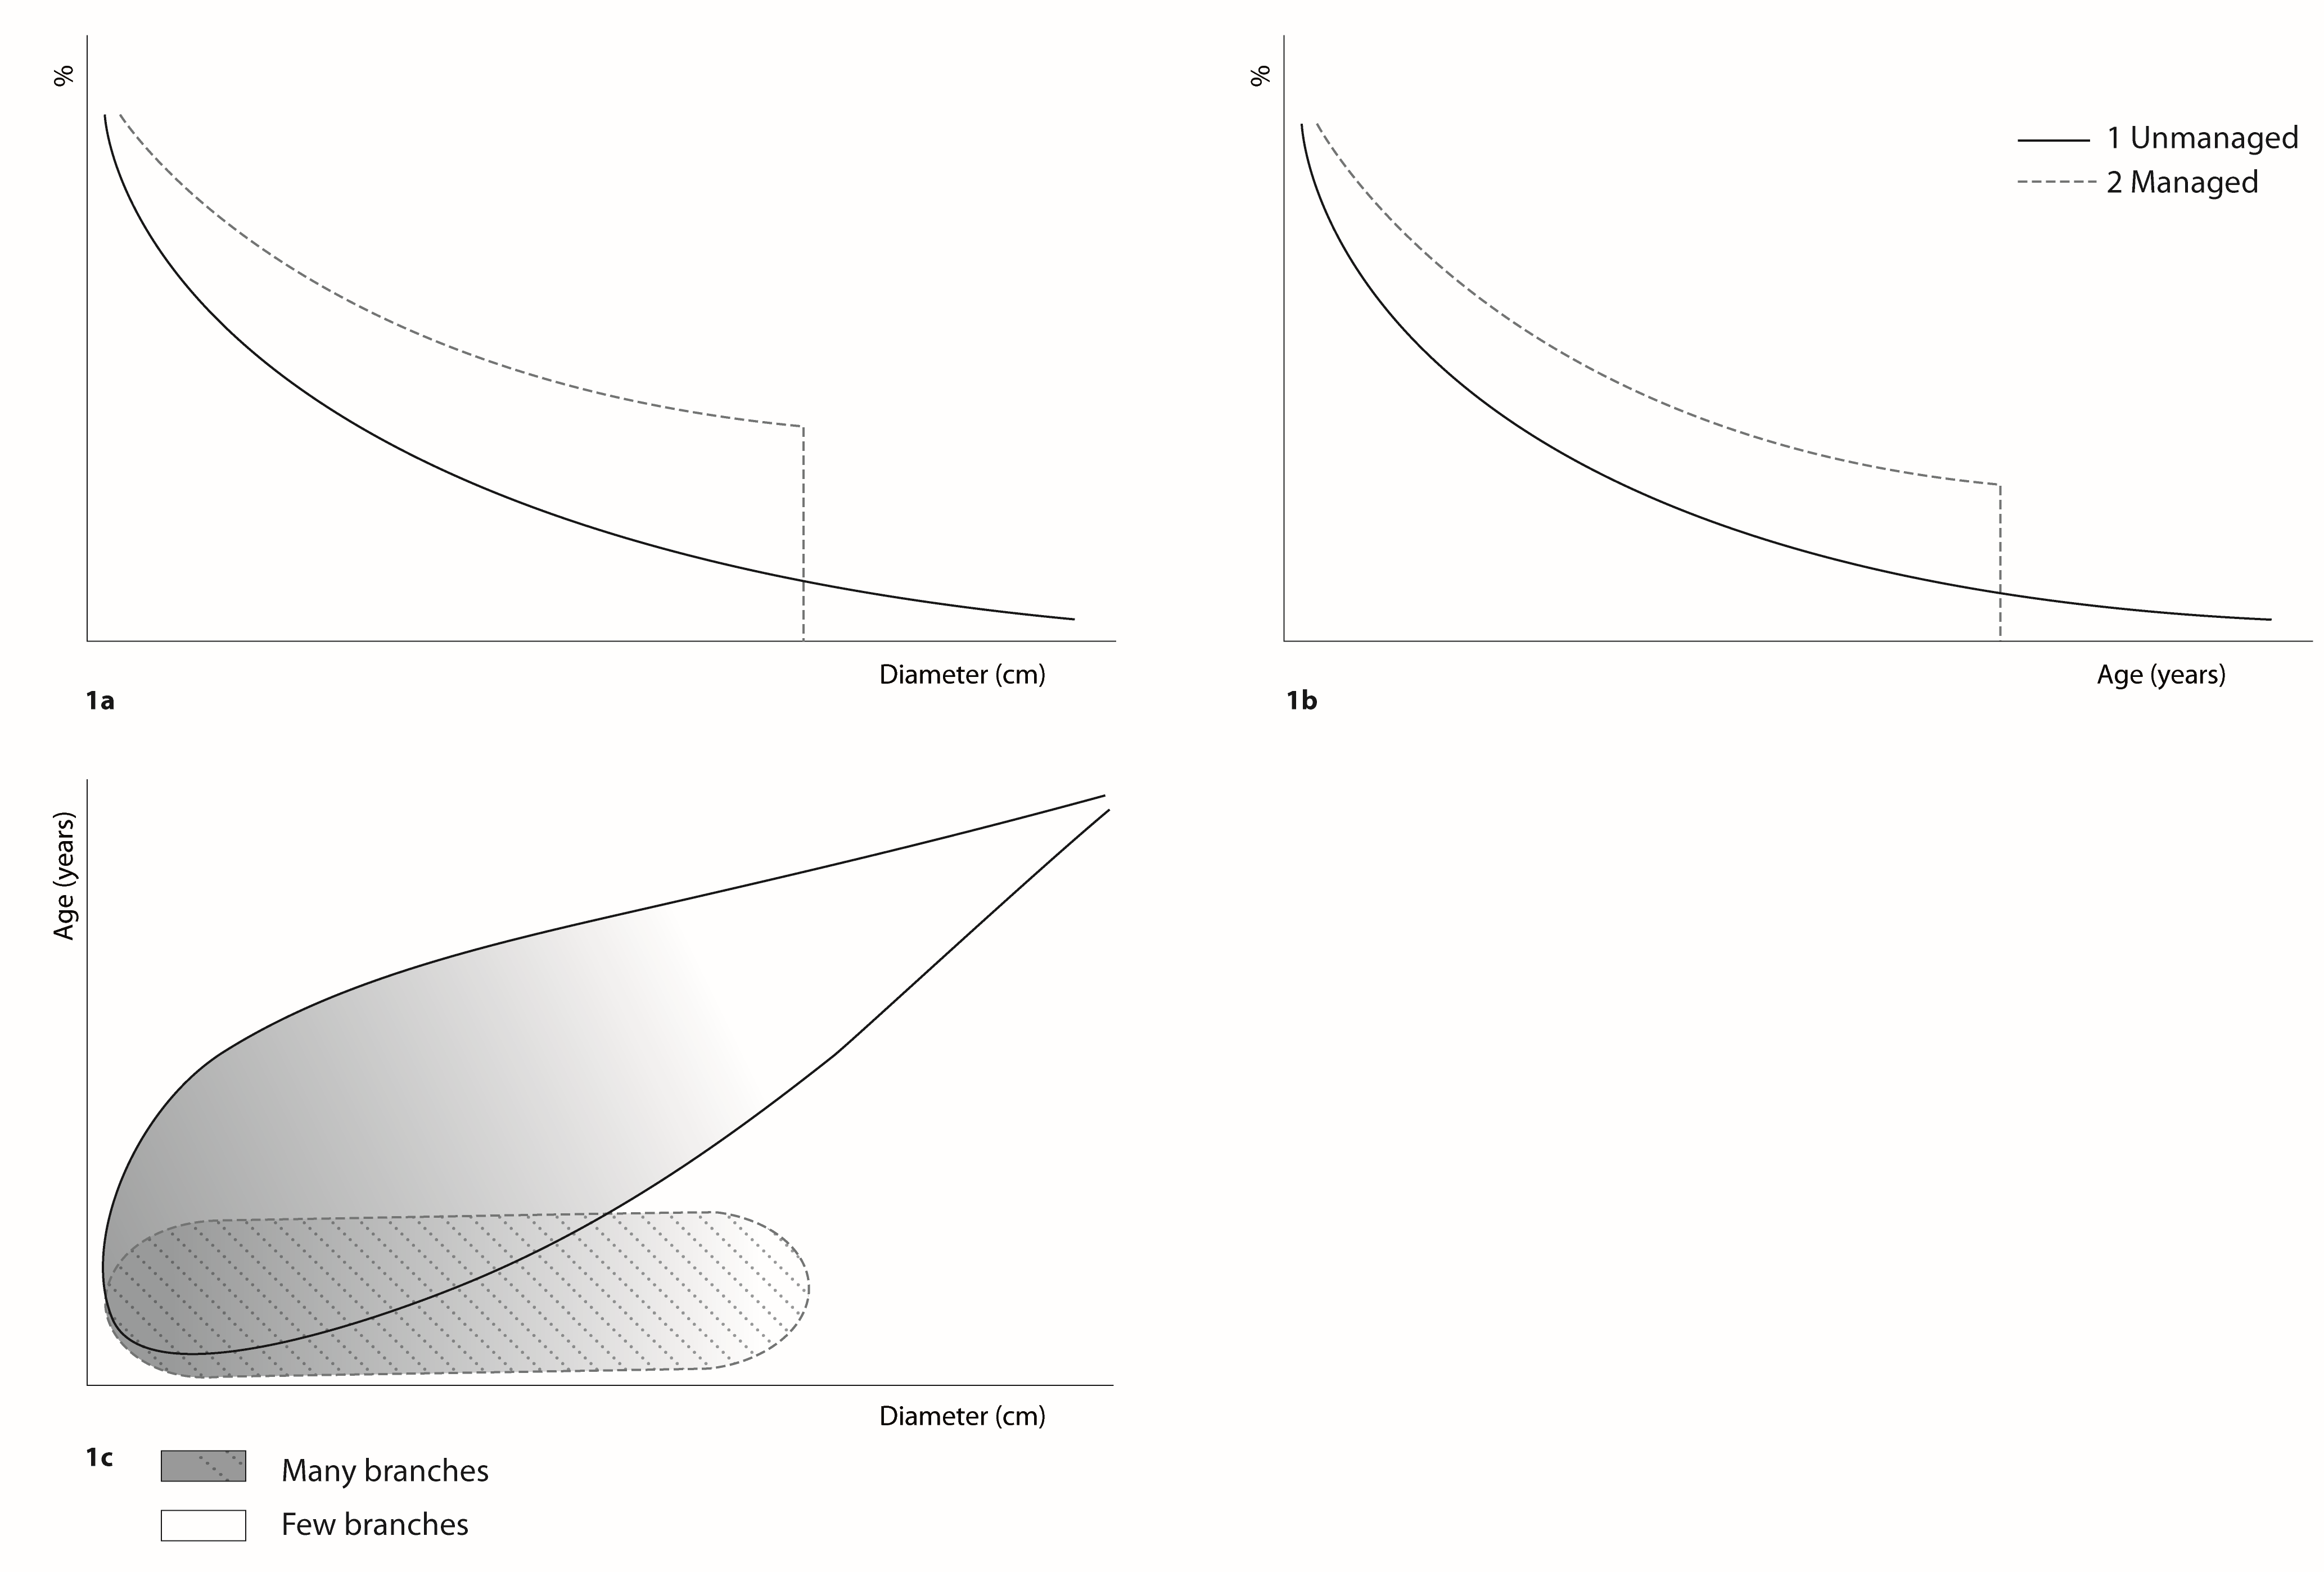
\includegraphics[width=0.9\textwidth,height=\textheight]{./figures/Vermeeren.png}
\caption{figure 1: growth model of managed (hatched) and unmanaged wood/trees, combination of diameter and age.}
\end{figure}

\hypertarget{session-2-shipwrecks-and-archaeological-structures}{%
\chapter*{Session 2: Shipwrecks and archaeological structures}\label{session-2-shipwrecks-and-archaeological-structures}}
\addcontentsline{toc}{chapter}{Session 2: Shipwrecks and archaeological structures}

\hypertarget{s2-o-001}{%
\section*{S2-O-001}\label{s2-o-001}}
\addcontentsline{toc}{section}{S2-O-001}

\textbf{Wood identification and dendrochronological techniques applied for the study of shipwrecks on the Atlantic coast of Argentina: comparison of different case studies showing limitations and potentials}

Ignacio A. Mundo\textsuperscript{1,~2}

\textsuperscript{\emph{1}} \emph{Laboratorio de Dendrocronología e Historia Ambiental, IANIGLA/CONICET, Mendoza, Argentina. \textsuperscript{2} Facultad de Ciencias Exactas y Naturales, Universidad Nacional de Cuyo, Mendoza, Argentina.}

\href{mailto:iamundo@mendoza-conicet.gob.ar}{\nolinkurl{iamundo@mendoza-conicet.gob.ar}}

Wood anatomy or xylogeny allows the botanical identification of woody material based on the recognition and quantification of various wooden traits. In the case of archaeology, and in particular for nautical archaeology, the wood anatomy provides information on the possible origin of nautical structures based on the range of distribution of woody plants, allows the association between the function fulfilled by a piece within a vessel and the mechanical properties of the wood, and it also helps to evaluate aspects related to the availability of timber and the building technology of a shipwreck, among others. In a nautical archaeological sense, dendrochronology analyses the information recorded in tree rings of timbers, which allows the dating of woody materials used in ship building, as well as estimating their possible origin (i.e.~dendroprovenancing). In this context, the interdisciplinary work between these three disciplines (xylogeny, dendrochronology and nautical archaeology) has only recently been applied in Argentina, despite the existence of a large number of woody nautical remains on the extensive Atlantic coast of this country. Through the analysis of different case studies carried out in the last years, this presentation aims to present and discuss the scope and limitations of the wood anatomy analyses in underwater archaeological studies in Argentina as well as to emphasize the dendroarchaeological potential of some of the materials found. The characteristics of the materials analysed in each case will be summarised, highlighting the limitations encountered and the potentialities for future studies.

\hypertarget{s2-o-002}{%
\section*{S2-O-002}\label{s2-o-002}}
\addcontentsline{toc}{section}{S2-O-002}

\textbf{Piers, wharfs and shipping at Masthugget, Gothenburg -- Investigating private harbours through wood and stone structures}

Andrine Nilsen\textsuperscript{1}

\textsuperscript{\emph{1}} \emph{Rio Göteborg Natur- \& kulturkooperativ, Gothenburg, Sweden.}

\href{mailto:andrine.nilsen@riogbg.se}{\nolinkurl{andrine.nilsen@riogbg.se}}

The harbour area Masthugget have large timber collections and stone structures as its main archaeological features. This contract archaeological project investigates how the built environment changes in character in different parts of the harbour from enterprise oriented to large private estates with lush gardens. The dendrochronological analysis is of vital importance to the project linked to dating, wood provenance analysis, the inquiry into timber supplies as well as for the study of the reconstruction and development of the harbour. Dendrochronology also plays part in the dating of the building stock on the piers and plots. Other dating tools used to track the 17-19th century are archaeological finds analysis combined with historical maps of the area.

Most plots and piers were private, and the owners were to a high degree well-known tradesmen many with Scottish origin. The city also owned two of the piers, one used as an iron-weighing station. In many ways, the harbours expands and benefits from international trading blockades connected to wars between England, France and North America affecting the colonial trade. The harbour was used for the import of colonial goods while exports such as tea, herring, iron and whale-oil were the most important. Other significant exports were timber and masts (which gave the harbour its name).

The project aims to find out how this foremost private harbour changed over time, how it was used, what the building stock of the piers looked like and how the buildings connected to the various enterprises of the area.

\hypertarget{s2-o-003}{%
\section*{S2-O-003}\label{s2-o-003}}
\addcontentsline{toc}{section}{S2-O-003}

\textbf{Marking time in the Iron Age; the dendrochronology of loch (lake) settlement in SW Scotland}

Anne Crone\textsuperscript{1}

\textsuperscript{\emph{1}} \emph{AOC Archaeology Group, Unit 7A Edgefield Industrial Estate, Loanhead, Midlothian, Scotland.}

\href{mailto:anne.crone@aocarchaeology.com}{\nolinkurl{anne.crone@aocarchaeology.com}}

Although there is evidence for settlements in the lochs of Scotland from the Neolithic to the early modern period, the 1st millennium BC saw the most intense period of activity, specifically that period from 800 to 400 BC where the calibration curve is so flat as to render radiocarbon determinations highly imprecise. Studies of the Iron Age throughout Europe are bedevilled by the Halstatt Plateau but in the British Isles few sites of that period have benefitted from the precision of dendro-dating. However, in a small area of SW Scotland, there are now three dendro-dated wetland settlements which are enabling archaeologists to examine the dynamics of regional settlement development via the chronological relationships between these sites. Extensive excavations at one of these sites, Black Loch of Myrton, yielded large quantities of oak, alder, hazel and ash, all of which have been analysed to produce a precisely dated chronological framework spanning three major episodes of occupation on the settlement, from 438/7 BC to 223 BC. Over the course of two centuries we see the development, expansion, abandonment and re-occupation of the settlement, all at the scale of human lifetimes.

In this talk the dendrochronological evidence from SW Scotland will be outlined, and some of the interpretative issues associated with the use of non-oak species will be raised. The impact of high-resolution timescales on our understanding of the dynamics of settlement in this period will also be explored.

\hypertarget{s2-o-004}{%
\section*{S2-O-004}\label{s2-o-004}}
\addcontentsline{toc}{section}{S2-O-004}

\textbf{Just bad quality? Some thoughts on the use of timber in medieval to modern shipbuilding}

Mike Belasus\textsuperscript{1}

\textsuperscript{\emph{1}} \emph{Lower Saxony Institute for Historical Coastal Research, Wilhelmshaven, Germany.}

\href{mailto:belasus@nihk.de}{\nolinkurl{belasus@nihk.de}}

The perception of wood in connection to shipbuilding of the past seems to be strongly idealised and often not fitting to the reality reflected in the archaeological context. Features of tree-anatomy were only sometimes recorded, and often ignored during the interpretation of ship finds. The idealized idea of a shipwright, who is choosing personally only the best material, was likely born out of an idealized image of the past and possibly influenced by rather recent shipbuilding practices. Detailed advise on the choice of high quality timbers for shipbuilding only appear in the 20th century, long after wood was superseded by steel for most vessels and competition for shipbuilding timber on the marked market had ceased. In some cases, this has produced a somewhat distorted interpretation of ships and shipbuilding because features of growth, in a holistic approach, can give information beyond timber quality but also on environmental influences and the human impact on this resource. In certain cases, it even allows to draw conclusions on economic and social circumstances. This way the information gathered from the building timber can alter the vessels interpretation.

This paper will discuss the demands for shipbuilding timber and its quality in North Western Europe as a result of the ERC-TIMBER project (Grant agreement No.~677152). It aims to reflect on possible social, economic or environmental reasons for the shipwrights' choices.

\hypertarget{s2-o-005}{%
\section*{S2-O-005}\label{s2-o-005}}
\addcontentsline{toc}{section}{S2-O-005}

\textbf{Double checking double Dutch: A reassessment of the construction features of the early modern Scheurrak SO1 shipwreck}

Rik Lettany\textsuperscript{1} , Petra Doeve\textsuperscript{2}, Esther Jansma\textsuperscript{3}

\textsuperscript{\emph{1}} \emph{Department of World Archaeology, Faculty of Archaeology, Leiden University, Leiden, the Netherlands. \textsuperscript{2} BAAC Archeologie en Bouwhistorie, the Netherlands. \textsuperscript{3} Cultural Heritage Agency of the Netherlands.}

\href{mailto:h.lettany@arch.leidenuniv.nl}{\nolinkurl{h.lettany@arch.leidenuniv.nl}}

In 1984, the remains of a late 16th Century Dutch merchantman were discovered off the coast of Texel, the Netherlands. The excavation of the site, named Scheurrak SO1 after its location, started in 1988 and ended in 1997. With a strong focus on the ship's construction features, it became one of the pioneering projects of Dutch underwater archaeology.

The shipwreck exhibited several peculiar construction details which deviated from other contemporary European shipbuilding traditions. As such, the data recovered from the Scheurrak SO1 shipwreck contributed strongly to what in nautical archaeology became known as the Dutch Flush and the Double Dutch discourses. Dutch flush refers to the shell-first building sequence of Dutch carvel built ships, at a time that most shipbuilding traditions used a frame-first sequence. Double Dutch, then again, refers to a brief moment in time when Dutch flush ships were built with a double layer of planking. Scheurrak SO1 has been considered the earliest known example of this latter technique. Based upon very limited dendrochronological data, the initial hypothesis was that Scheurrak SO1 was built around 1580 with two layers of planking.

Reassessment of Scheurrak SO1's construction details within the frame of the interdisciplinary research project ``Scheurrak SO1 in the Maritime Cultural Landscape of the Early Modern Netherlands, 1550-1650'' at Leiden University, now suggests that the ship may have known multiple building phases. Re-analysis of the available tree-ring curves seems to support this, while analysis of additional samples demonstrate a more dispersed timber provenance than initially deduced. Although research is still ongoing, current results do challenge the known Double Dutch discourse and encourage a reinterpretation of the construction of the Scheurrak SO1 shipwreck.

\hypertarget{s2-o-006}{%
\section*{S2-O-006}\label{s2-o-006}}
\addcontentsline{toc}{section}{S2-O-006}

\textbf{From a forest to a ship and into a wreck, and back again?}

Minna Koivikko\textsuperscript{1}, Tuomas Aakala\textsuperscript{2}, Katariina Vuori\textsuperscript{3}

\textsuperscript{\emph{1}} \emph{Finnish Heritage Agency, Finland. \textsuperscript{2} Jyväskylä, Finland. \textsuperscript{3} Oulu, Finland.}

\href{mailto:minna.koivikko@museovirasto.fi}{\nolinkurl{minna.koivikko@museovirasto.fi}}

The aim of the project is to develop interpretation of so-called skeleton wrecks, i.e., wooden wrecks, which only have preserved partly, and no informative objects have been discovered. We are studing the relationship between a man and a forest through interpretation of wooden vessels.

The Lost Navy, Sweden's ``Blue'' Heritage c.~1450--1850 research programme aims to collect information about the ships in the fleet. It is a joint marine archaeology and - history project in the Baltic Sea region for 2021--2026. In Finland, the research sub-project focuses on wooden wrecks of the Swedish era fleet. The project has a multidisciplinary approach, combining archaeology with shipbuilding, dendrochronology, and forest studies.

\hypertarget{s2-o-007}{%
\section*{S2-O-007}\label{s2-o-007}}
\addcontentsline{toc}{section}{S2-O-007}

\textbf{House and Boat. Reuse of ship planking in a 10th century building at Hungate, York}

Steven J. Allen\textsuperscript{1}

\textsuperscript{\emph{1}} \emph{Conservation Department, York Archaeology, United Kingdom.}

\href{mailto:sallen@yorkat.co.uk}{\nolinkurl{sallen@yorkat.co.uk}}

In the course of excavations by York Archaeological Trust (Now York Archaeology) in 2008-9 at Hungate in York revealed the waterlogged timbers of another building of a type best known from Coppergate. This building, dating to the third quarter of the 10th century CE was superficially of the same construction as seen earlier at Coppergate and was a rectangular pit cut into the ground, lined with posts that supported a boarded outer lining.

At Coppergate, the timbers were largely freshly felled specifically for the buildings in which they were found and the tree ring sequences are local to the York region. However at Hungate, when the timbers were lifted, it was immediately apparent that the board lining was in fact made up of reused articulated slabs from a clinker-built boat.

Moreover, the type of clinker construction was unusual and not of the `typical' North West European/Scandinavian type. Dendrochronological samples allowed the identification of the potential source for the boat timbers, which was not local to York. This paper considers the evidence provided from the study of the woodworking technology and the work done to identify the type of boat, its potential provenance and indeed the provenance of the timbers used in its construction.

\hypertarget{s2-o-008}{%
\section*{S2-O-008}\label{s2-o-008}}
\addcontentsline{toc}{section}{S2-O-008}

\textbf{How a broken wooden board uncovered an early medieval mill}

Julia Weidemüller\textsuperscript{1}, Franz Herzig\textsuperscript{1}, Leander Schmidt\textsuperscript{1}, Jeremy Collacott\textsuperscript{1}

\textsuperscript{\emph{1}} \emph{Bayerisches Landesamt für Denkmalpflege, Thierhaupten, Germany.}

\href{mailto:julia.weidemueller@blfd.bayern.de}{\nolinkurl{julia.weidemueller@blfd.bayern.de}}

In September 2021, historic timbers were uncovered at a construction site in Aichach, Bavaria. The site was not designated as monument, therefore it was not accompanied archaeologically. Nevertheless, the construction company reported these finds to the Bavarian State Office for Monument Preservation (BLfD). The first pieces were examined in the internal laboratory for dendroarchaeology. The site could be identified as an early medieval mill on the basis of a broken paddle fragment. Subsequently, hundreds of timbers from several construction phases of the mill were excavated and documented in close cooperation between Construction Company, Archaeological Specialists and Dendroarchaeologists.

In addition to small finds such as paddles, vessels and tools, numerous construction timbers were found, many still in situ. For the first time, an intact mill pond, including dam, filter system and mill channel, could be excavated. In this case the wood species composition is exciting, since a large part of the construction timbers consisted of alder and beech. Only heavily used structures like the sluice gate or the substructures of the mill building were made of oak. The investigations have not yet been completed. First measurements date to the 8th and 9th centuries AD. A heavy flood event ended milling at this site.

A comprehensive archaeological evaluation is planned, including age structures and wood species composition. However, the sheer mass of the timbers would offer many more starting points for statistical analyses on early medieval forest structures and wood species selection, to name a few. Since there are no resources available at BLfD for research of this kind, I hope that the presentation of the project to expert circles will provide helpful comments and possibly lead to further research.

\hypertarget{s2-o-009}{%
\section*{S2-O-009}\label{s2-o-009}}
\addcontentsline{toc}{section}{S2-O-009}

\textbf{A dendroarchaeological study of Roman-period river barges from the Lower Rhine region}

Yardeni Vorst\textsuperscript{1}

\textsuperscript{\emph{1}} \emph{Vorst wood research, Zaandam, the Netherlands.}

\href{mailto:yvorst@gmail.com}{\nolinkurl{yvorst@gmail.com}}

In 2003, a river barge dating to the Roman period was found in a former riverbed of the Rhine in the western part of the Netherlands. The ship, named `Woerden 7', formed a new discovery in a long series of Roman-period ship finds in Lower Rhine region since the late 1960's. In particular, large flat-bottomed river barges had been found. Many of these vessels were excavated and some were conserved, such as the The Zwammerdam ships, found in the village of Zwammerdam in the 1970's. For a research project these ships have been re-examined using more modern techniques. A comparison between ship Zwammerdam 6 and the earlier mentioned Woerden 7 vessel shows that the ships resemble each other closely in construction. Apart from a study of the ship constructions a dendroarchaeological study of the timbers has been undertaken. Dendrochronology has been used to date the ships and to determine which timbers were obtained from the same trees. This has helped to trace original building sequences and allowed for new ideas on the shipbuilding processes. Identifying the source area of trees used in this Roman-period shipbuilding, i.e.~the provenance of the timbers will be presented in an other paper together with Ronald Visser. The Zwammerdam vessels are currently being reconstructed at an archaeological park (Archeon) in the South of Holland and the research information gathered will contribute to stories on their historical background.

\hypertarget{s2-p-001}{%
\section*{S2-P-001}\label{s2-p-001}}
\addcontentsline{toc}{section}{S2-P-001}

\textbf{Conservation processes of a painted wooden coffin at Saqqara area}

Abdelmoniem M. Abdelmoniem\textsuperscript{1}, Naglaa Mahmoud\textsuperscript{1}, Wael S. Mohamed\textsuperscript{2}

\textsuperscript{\emph{1}} \emph{Conservation Department, Faculty of Archaeology, Fayoum University, Fayoum, Egypt. \textsuperscript{2} Polymer department, National Research Centre, Dokki, Giza, Egypt.}

\href{mailto:ama63@fayoum.edu.eg}{\nolinkurl{ama63@fayoum.edu.eg}}

This paper aims to document the conservation processes of a polychrome wooden coffin at Saqqara dating back to the late period. The exterior part of the coffin is decorated with painted layer, while inside it is covered with a layer of the black resin.

The coffin was in a bad condition. It was covered with a thick layer of dust, loosing parts of the painted and gesso layers, as well as other parts of these layers were lost. Some parts were missing from the foot area of the lid coffin. 2D illustrations and 3D modules were made to document the coffin.

The conservation processes of the wooden coffin included mechanical and chemical cleaning, reattachment of the separated parts of the ground layer and painted layers, filling the edge of the painted layer, and consolidating the black resin layer. The materials used for these processes proved to be stable and retrieval by many researchers.

The conservation process included mechanical cleaning using soft brushes, chemical cleaning using ethyl alcohol and water for painted layer and xylene and water for black resin layer, stabilization of the separated gesso layer using Paraloid B72, filling cracks of the gesso layers using glass microballoon with Paraloid B72, and consolidating the painted layer with KlucelE and black resin layer with Nano Paraloid B72.

\hypertarget{s2-p-002}{%
\section*{S2-P-002}\label{s2-p-002}}
\addcontentsline{toc}{section}{S2-P-002}

\textbf{Microscopy techniques for the examination of waterlogged archaeological wood}

Angela Balzano\textsuperscript{1}, Maks Merela\textsuperscript{1}, Katarina Čufar\textsuperscript{1}

\textsuperscript{\emph{1}} \emph{Biotechnical Faculty, University of Ljubljana, Ljubljana, Slovenia.}

\href{mailto:Angela.Balzano@bf.uni-lj.si}{\nolinkurl{Angela.Balzano@bf.uni-lj.si}}

Waterlogged archaeological wood (WAW) from prehistoric pile-dwelling settlements in Ljubljansko barje, Slovenia, was examined using various microscopic techniques. We have performed light microscopy (LM) using bright field, polarization and fluorescence modes with different sample preparation methods (cutting of frozen WAW, cutting after embedding in paraffin). Unstained and stained sections with safranin and astra blue or acridine orange and chrysoidin were considered. We have developed an improved protocol for scanning electron microscopy (SEM) and energy dispersive X-ray spectroscopy (EDX) based on the observation of sections obtained with a razor blade from frozen samples and fixed with albumin on sample supports to prevent cracking and collapse of the highly degraded wood. Advantages of applied techniques will be shown for WAW of Quercus, Faxinus, Acer, Salix and Populus with an age of about 4,500 years.

Sections from frozen WAW, approximately 20-30 µm thick and 1cm2 in size, allowed recognition of cellular and tissue level structures with LM. Embedding in paraffin provided thinner but smaller sections which tended to tear.

The improved SEM protocol provided high quality images of large sections at lower magnifications and also of details at high magnifications with high resolution. The combination of SEM and EDX allowed the observation of the preservation of the cell wall as well as the location, amount, shape and chemical composition of various inclusions with high amounts of Fe, S and Ca found in all taxa studied, while \emph{Populus} also contained increased amounts of Si.

\hypertarget{s2-p-003}{%
\section*{S2-P-003}\label{s2-p-003}}
\addcontentsline{toc}{section}{S2-P-003}

\textbf{Practices of shipwreck timber sampling for dendrochronology}

Daniel Peter Dalicsek\textsuperscript{1}

\textsuperscript{\emph{1}} \emph{Moesgård Museum, Aarhus, Denmark.}

\href{mailto:dad@moesgaardmuseum.dk}{\nolinkurl{dad@moesgaardmuseum.dk}}

In 2018, two important publications saw light, Selecting and Sampling Shipwreck Timbers for Dendrochronological Research: practical guidance by Daly et al.~and Shipwrecks and Provenance: in-situ timber sampling protocols, with a focus on wrecks of the Iberian shipbuilding tradition by Rich et al.~My presentation would look at the impact of these publications and the focus on the works of maritime archaeologists and dendrochronologists in sampling shipwreck timbers over the past five years. It´s main focus would be on intrusive survey methods and on shipwreck sites, but would not exclude other underwater sites or terrestrial excavations. It would consist of a survey questionnaire, sent out to maritime archaeologists across the globe and interviews with maritime archaeologists and dendrochronologists ahead of the conference. This would enable insight and provide an overview over fieldwork practices today. The presentation would showcase the opportunities for better and more uniform sampling practices as well as present a chance for and generate discussion among the conference´s audience. The aim is to take a snapshot of how we conduct our science and if collaboration between dendrochronologists and archaeologists is sufficient.

\hypertarget{s2-p-004}{%
\section*{S2-P-004}\label{s2-p-004}}
\addcontentsline{toc}{section}{S2-P-004}

\textbf{The Gribshunden Barrels}

Anton Hansson\textsuperscript{1}, Hans Linderson\textsuperscript{1}, Brendan Foley\textsuperscript{2}

\textsuperscript{\emph{1}} \emph{The Laboratory of Wood Anatomy and Dendrochronology, Department of Geology, Lund University, Lund, Sweden. \textsuperscript{2} Department of Archaeology and Ancient History, Lund University, Lund, Sweden.}

\href{mailto:anton.hansson@geol.lu.se}{\nolinkurl{anton.hansson@geol.lu.se}}

The Danish Royal Flagship Gribshunden sank in the Blekinge archipelago in the early summer of 1495, while on its way to the Swedish town of Kalmar. There the Danish King Hans planned to meet the Swedish Regent Sten Sture the Elder in the kings wish to re-establish the Nordic Union between Denmark, Norway, and Sweden by being elected king of Sweden. During field campaigns in 2019 and 2021 a joint multi-disciplinary research effort led by Lund University has excavated parts of the Gribshunden shipwreck. As a part of the excavations, a large number of barrels staves and heads were recovered for dendrochronological and dendroprovenance analysis in order to answer certain research questions: (i) the timber source area (ii) The barrel construction locality (iii) the lifespan of a barrel (iiii) barrel size and standards. In total, 135 oak staves and heads were analysed, 79 \% of which were successfully dated. Two major timber source areas were revealed, Baltic (59\%) and Scania (22\%). The mix of timber sources in the barrels suggest they were not constructed in the source area. Based on the average sapwood amount we can conclude that most barrels must have been constructed a few years prior to sinking, suggesting a short life span of barrels in general. Together with these dendrochronological results, further studies on numerous finds at the wreck site will provide new views of the medieval economy and political connections in the late medieval period.

\hypertarget{s2-p-005}{%
\section*{S2-P-005}\label{s2-p-005}}
\addcontentsline{toc}{section}{S2-P-005}

\textbf{Connecting ships: using dendrochronological network analysis to determine provenance and ship building practices of Roman-period river barges found in the Lower Rhine region}

Ronald M. Visser\textsuperscript{1}, Yardeni Vorst\textsuperscript{2}

\textsuperscript{\emph{1}} \emph{Archaeology, School of Business, Building and Technology, Saxion - University of Applied Sciences, Deventer, Netherlands. \textsuperscript{2} Vorst wood research, Zaandam, the Netherlands.}

\href{mailto:r.m.visser@saxion.nl}{\nolinkurl{r.m.visser@saxion.nl}} - \href{mailto:yvorst@gmail.com}{\nolinkurl{yvorst@gmail.com}}

Over the past decades various Roman-period river barges were found in the Lower Rhine region. These ships were large vessels of over twenty meters in length. Many were excavated in order to document the constructions and some were lifted from the ground and conserved for future display. The first barges that were found (fifty years ago), the Zwammerdam ships, were among those that were preserved. This has more recently allowed for a re-examination of their ship constructions using more modern techniques. Research on the constructions including a dendroarchaeological study of the timbers has been undertaken by Y. Vorst. The provenance of the wood has been studied by both researchers, based on a recently published approach (Visser 2021). This approach uses networks to visualize and explore dendrochronological relations based on similarity. In addition, these networks give insight in other aspects of ship building practices, such as wood use and the construction. The combined studies have led to a better understanding of past practices in shipbuilding and timber transport and use during the Roman period.

Visser, R.M. 2021 Dendrochronological Provenance Patterns. Network Analysis of Tree-Ring Material Reveals Spatial and Economic Relations of Roman Timber in the Continental North-Western Provinces. \emph{Journal of Computer Applications in Archaeology} 4(1): 230--253. DOI: \url{https://doi.org/10.5334/jcaa.79}.

\hypertarget{session-3-furniture-and-works-of-art}{%
\chapter*{Session 3: Furniture and works of art}\label{session-3-furniture-and-works-of-art}}
\addcontentsline{toc}{chapter}{Session 3: Furniture and works of art}

\hypertarget{s3-o-001}{%
\section*{S3-O-001}\label{s3-o-001}}
\addcontentsline{toc}{section}{S3-O-001}

\textbf{Musical string instruments: Tree-ring dating and provenancing to verify their authenticity}

Paolo Cherubini\textsuperscript{1,~2}, Bruce Carlson\textsuperscript{3}, Wolfgang Talirz\textsuperscript{4}, Malcolm H. Wiener\textsuperscript{5}

\emph{\textsuperscript{1} Dendrosciences, Swiss Federal Institute for Forest, Snow and Landscape Research WSL, Birmensdorf, Switzerland. \textsuperscript{2} Department of Forest and Nature Conservation, Faculty of Forestry, University of British Columbia, Vancouver BC, Canada. \textsuperscript{3} Luthier, via Amilcare Ponchielli 11, Acquanegra Cremonese (Cremona), Italy. \textsuperscript{4} Musician, violist, Berliner Philharmoniker, Berlin, Germany. \textsuperscript{5} Institute for Aegean Prehistory, Greenwich, CT, United States of America.}

\href{mailto:paolo.cherubini@wsl.ch}{\nolinkurl{paolo.cherubini@wsl.ch}}

The prime factor which affects the market value of a work of art is its authenticity. String instruments are among the most valued works of art, particularly those made by the old violinmaking masters of northern Italy in the late 17th and early 18th centuries. Their authenticity is difficult to be verified on the basis of style and design alone, as these were often copied or forged. The only analysis that can objectively indicate, if not the exact year an instrument was made, at least the date before which it certainly was not made is a dendrochronological analysis of the wood used to make the instrument. We will review the dendrochronological studies done to assess the authenticity of the instruments made by the old Italian masters, bringing the example of the controversial dating of the famous violin

"The Messiah" attributed to Antonio Stradivari. Such studies help to establish the earliest date the tree from which the wood was taken could have been felled, and to determine the source region of the wood. We will present the main achievements and challenges that have arisen in the past 50 years, and discuss the limitations and potential of using dendrochronological methods to establish the provenance and time period in which an instrument was made. Finally, we will describe needs of research in history, wood anatomy, biochemistry and dendrochronology, proposing some new methods that may open up new avenues of research and aid in the assessment of the authenticity of old string instruments

\hypertarget{s3-o-002}{%
\section*{S3-O-002}\label{s3-o-002}}
\addcontentsline{toc}{section}{S3-O-002}

\textbf{Three altarpieces attributed to the Borman dynasty studied by dendrochronology}

Pascale Fraiture\textsuperscript{1}, Christophe Maggi\textsuperscript{1}, Lisa Schindo\textsuperscript{1,~2}

\emph{\textsuperscript{1} Laboratories department (Dendrochronology Lab), Royal Institute for Cultural Heritage (KIK-IRPA), Brussels, Belgium. \textsuperscript{2} ROOTS Cluster of Excellence, Institute of Pre- and Early Prehistoric Archaeology, Christian-Albrechts-University, Kiel, Germany.}

\href{mailto:pascale.fraiture@kikirpa.be}{\nolinkurl{pascale.fraiture@kikirpa.be}}

Since 2010, the Dendrochronological Laboratory of the KIK-IRPA have had the opportunity to study three sculpted altarpieces attributed to the Borman dynasty.

The first was the Altarpiece of the Coronation of the Virgin of the church of the Assumption in Errenteria (ES), analyzed during its conservation-restoration treatment by Albayalde S.L. (Donostia-San Sebastián). It is dated by a painted inscription 1528. The second is the Saint Denis Altarpiece of the Collegial church of St-Denis in Liège (BE), attributed around 1520-1530, which was the object of an interdisciplinary study and conservation-restoration treatment at the KIK-IRPA in 2012-2014. The third is the Saint George Altarpiece now conserved at the Royal Museums of Art and History, Brussels (BE), which contains a sculpted date 1493, also analyzed in the frame of its study and treatment at the KIK-IRPA between 2018 and 2021.

For all of them, the dendrochronological analysis during a conservation-restoration treatment allowed the study of sculpted elements as well as elements from boxes and architectural decoration. Next to tree-ring dating issues, this presentation would enlighten the supplying conditions for wood, that is, the geographical provenance of the oak and the quality selection of the trees used for the different parts of the altarpieces, as well as the woodworking techniques and the know-how of the craftsmen who produced these works. Comparisons of the observations done on the three ensembles, which have different genesis and materiel history, will also be discussed, as they reveal important differences even though they come from the same workshop.

\hypertarget{s3-o-003}{%
\section*{S3-O-003}\label{s3-o-003}}
\addcontentsline{toc}{section}{S3-O-003}

\textbf{Old doors deserve attention of dendrochronologists: first examples from Estonia}

Alar Läänelaid\textsuperscript{1}, Aoife Daly\textsuperscript{2}, Kristina Sohar\textsuperscript{1}

\emph{\textsuperscript{1} Institute of Ecology and Earth Sciences, University of Tartu, Tartu, Estonia. \textsuperscript{2} SAXO-Institute, University of Copenhagen, Copenhagen, Denmark.}

\href{mailto:alar.laanelaid@ut.ee}{\nolinkurl{alar.laanelaid@ut.ee}}

During recent years five old doors have been brought to focus of attention in Estonia. The earliest of them appeared to be the door of the King's Chapel in Tallinn Dome. The door consists of vertical pine planks covered with horizontal oak planking that were both dated. Some details indicate that the door was manufactured for a smaller doorway and the oak boards were added later.

The door from a mediaeval town prison locates in the Bremen Tower of the town wall of Tallinn. This is an oak door of three vertical planks, armoured by iron hinges. The date of the door, 1392 tpq, specifies the written, known building period of the Bremen Tower.

The decorated door from a chapel of von Maydell's family at Velise manor has an obscure history. The pine door with coats of arms of two nobility families was dated to 1524 tpq, while the chapel was erected in the 1880s. Presumably the door was brought to the chapel from Tallinn (Reval). Origin of the pair of doors could be explained by investigating the real estate of these families in mediaeval Reval.

In a flat in Tallinn Old Town there are two inner doors with historical appearance. These are board doors with door leafs in the frame. One of these doors, dated 1523 tpq, distinguishes by its special hinges that were in fashion in the 17th century. The other door is under examination yet. There are several details giving hints on their age.

\hypertarget{s3-o-004}{%
\section*{S3-O-004}\label{s3-o-004}}
\addcontentsline{toc}{section}{S3-O-004}

\textbf{Japanese art through time: a dendrochronological investigation into cultural progression through Netsuke}

Antoinette Marie Piotrowska Lawrence-Cooper\textsuperscript{1}

\emph{\textsuperscript{1} Geography, Student, University of Cambridge, Cambridge, United Kingdom.}

\href{mailto:amp213@cam.ac.uk}{\nolinkurl{amp213@cam.ac.uk}}

In this research project, I will be using principles of dendrochronology and macroscopic analysis to study the wood anatomy of Japanese Netsuke (small wooden sculpture) in possession of the Fitzwilliam Museum. Upon uncovering the tree species, I attempt to locate the spatial (regional) origin of the artefact. Subsequently, I aim to connect the period of its creation and material with relevant historical and cultural developments in Japan. This research project aims to explore the extent to which interconnectivity between nature and cultural progression can be analysed non-invasively. During the Tokugawa period (1603--1868), netsuke were an indispensable item of dress, therefore, many species of wood from a range of climates were desired for their aesthetic value. Furthermore, cultural development was at an all-time high, with the rise of woodblock printing. As a result, this project investigates an item worn by all classes of citizens and how cultural development can be traced. The technique used to analyse the wood was macroscopic analysis based on Crivellaro \& Ruffinatto (2019). Wood species was identified by locating the cross-section, and coding anatomical features such as vessel \& parenchyma cell arrangements then cross-referencing them against the International Association of Wood Anatomists (IAWA) database. It must be noted that this research project is currently ongoing and will be completed by the first week of April.

\hypertarget{s3-o-005}{%
\section*{S3-O-005}\label{s3-o-005}}
\addcontentsline{toc}{section}{S3-O-005}

\textbf{The journey of nudsugana. Archaeobotanical study of the wooden sculptures from Gunayala (Panama) located at the Världskulturmuseet in Göterborg (Sweden)}

Nuria Romero Vidal\textsuperscript{1}

\emph{\textsuperscript{1} History Department, Faculty of Geography and History, University of Santiago de Compostela, Santiago de Compostela, Spain.}

\href{mailto:nuriaromerovidal@gmail.com}{\nolinkurl{nuriaromerovidal@gmail.com}} - \href{mailto:nuriaromero.vidal@usc.es}{\nolinkurl{nuriaromero.vidal@usc.es}}

The \emph{nudsugana} are subjectivized sculptures with their own life and agency which are carved by the Gunadule communities to embody the properties of the trees. Gunadule people carve them into anthropomorphic and zoomorphic forms, humanizing them without changing their nature. Large number of them have travelled across the Atlantic Ocean since the 19th century and they have ended up in the European ethnographic collections. The Världskulturmuseet has the largest number of these carvings, which have not been studied yet. Within the PhD thesis From tree to object, which aims to integrate archaeobotany and anthropology besides state-of-the-art digital tools in the study of wooden objects produced by the Gunadule people, these pieces will be studied to explore all the possibilities offered by the archaeometric analysis of these objects. As each nudsugana is named after the tree from which it was carved, we have already a list of 20 different taxa that are part of a catalogue in which we are including uses, properties, ecology data and anatomical features with the main aim of developing a multidisciplinary methodology to improve the anatomical study in tropical woods. We present the multidisciplinary methodology-wood analysis, SEM with EDX, Py-GC-MS, FTIR, μCT- that is intended to be carried out on this study and the first advances of the thesis project by inquiring what nudsugana can tell us about the people, forests, and trees where they come from and also, helping them to start their journey back home.

\hypertarget{s3-o-006}{%
\section*{S3-O-006}\label{s3-o-006}}
\addcontentsline{toc}{section}{S3-O-006}

\textbf{Looking into Rijksmuseum's maritime collection: provenance and function of 18th and 19th century half hull models}

Tirza Mol\textsuperscript{1}, Paul van Duin\textsuperscript{2}, Jeroen ter Brugge\textsuperscript{3}, Marta Domínguez-Delmás\textsuperscript{4}

\emph{\textsuperscript{1} Shipmodel and furniture conservator at Rijksmuseum, Amsterdam, The Netherlands. \textsuperscript{2} Head of furniture conservation at Rijksmuseum, Amsterdam, The Netherlands. \textsuperscript{3} Curator of maritime collections at Rijksmuseum, Amsterdam, The Netherlands. \textsuperscript{4} Institute of Art History, Faculty of Humanities, University of Amsterdam, Amsterdam, The Netherlands.}

\href{mailto:T.Mol@rijksmuseum.nl}{\nolinkurl{T.Mol@rijksmuseum.nl}}

The maritime collection of the Rijksmuseum (Amsterdam) contains around 1800 navy related models, including circa 300 half hull ship models. A half model is a scale model from the starboard or portside half of a ship hull, mounted on a wooden backboard. It is constructed in wood, polychromed and finished with a transparent varnish. Sometimes a label is attached to the backboard, with information on the scale, name or provenance of the model. In the 18th and 19th centuries half models were produced on ship wharfs all over the Netherlands.

Despite the great number of half models in the Rijksmuseum collection, little is known about their production and function. Many models are not attributed to a specific dockyard, are not associated with actual ships, and have therefore been assigned broad production date ranges. This paper describes how systematic technical research can contribute to the knowledge about the provenance of the half models and their possible role in the Dutch maritime shipbuilding industry.

A reconstruction of a half model was made to understand the construction sequence. Visual inspection and tool traces recording were used to study the construction process, and dendrochronological research was used to date the models and establish their potential production shipyard. By clustering the models according to stylistic features, materials and tool traces, as well as dendrochronological data, we have been able to attribute groups of them to specific shipyards and to connect some of them to actual ships. This paper shares the preliminary results of this fascinating research.

\hypertarget{s3-o-007}{%
\section*{S3-O-007}\label{s3-o-007}}
\addcontentsline{toc}{section}{S3-O-007}

\textbf{Dating Northern-Netherlands cabinets from the late 17th century}

Paul van Duin\textsuperscript{1}, Iskander Breebaart\textsuperscript{1}, Marta Domínguez-Delmás\textsuperscript{1,~2}

\emph{\textsuperscript{1} Conservation and Science Department, Rijksmuseum, Amsterdam, The Netherlands. \textsuperscript{2} Institute of Art History, Faculty of Humanities, University of Amsterdam, Amsterdam, The Netherlands.}

\href{mailto:p.van.duin@rijksmuseum.nl}{\nolinkurl{p.van.duin@rijksmuseum.nl}}

Over the last 30 years, a great number of pieces of furniture from the Rijksmuseum collection (Amsterdam, The Netherlands) have been dated by dendrochronology. Furniture from the Northern Netherlands was seldom dated by the maker, and never signed, and few documents have survived that could indicate who made it and when. A very popular type of cabinet around the 1700s was a cabinet on a stand, with large flat surfaces decorated with marquetry with flowers and/or geometrical patterns. An ongoing project aims to identify groups of cabinets that were produced by a same maker, based on similarities in the construction and decorative features, and on dendrochronological dates and groupings of the oak (Quercus sp.) components.

Here, we will present the process followed to date the cabinets, from the selection of components to be analysed to the interpretation of the dendrochronological results. A selection of 15 pieces includes the first cabinet ever dated by dendrochronology in the Rijksmuseum, the dolls' house of Petronella Oortman, as well as furniture by Jan van Mekeren with intricate marquetry depicting large bouquets of flowers. Dating furniture differs from dating panel paintings or sculptures, as a cabinet on average consists of 50 to 100 wooden components. In many of those components the end grain is not accessible, or partial dismantling is needed to access it, hence conscious choices must be made. The dates and provenance of the wood have been compared to previously existing art-historical dates, to assess the added value of dendrochronological dating and the contribution of this science to understanding developments in cabinetmaking.

\hypertarget{s3-o-008}{%
\section*{S3-O-008}\label{s3-o-008}}
\addcontentsline{toc}{section}{S3-O-008}

\textbf{Unravelling a North Netherlandish 17th-century panel maker}

Jørgen Wadum\textsuperscript{1,~2}, Marta Domínguez-Delmás\textsuperscript{3}, Angela Jager\textsuperscript{4}

\emph{\textsuperscript{1} Nivaagaard Collection, Nivå, Denmark. \textsuperscript{2} Wadum Art Technological Studies (WATS), Vanlose, Denmark. \textsuperscript{3} Institute of Art History, Faculty of Humanities, University of Amsterdam, The Netherlands. \textsuperscript{4} RKD -- Netherlands Institute for Art History, The Hague, The Netherlands.}

\href{mailto:WATS@jorgenwadum.com}{\nolinkurl{WATS@jorgenwadum.com}}

The marking and branding of oak painting supports is a well-known practice in Antwerp in the 16th and 17th centuries. Conversely, information about the activities and regulations of 17th-century panel makers in the Northern Netherlands is scant and has hitherto never been thoroughly researched.

This paper presents a panel maker who sold his products to painters within the Dutch Republic. He stamped his house mark in the back of the panels: two letters `M' above each other and crowned by the cipher `4'. This mark has been found in panels from several painters active between 1632 and 1648.

To narrow down the location of the unknown panel maker's workshop, we investigate his source of timber and the eventual interrelationships between the planks used for one or more panels. In addition, we study the painters who painted on his supports. As such, this paper for the first time presents a thorough dendrochronological examination of seven of his 15 known panels combined with art historical research into the works of his customers. Based on the provenance of the wood of the panels, the painters who used them and the supply of timber to the Dutch Republic in the second half of the 17th century, we propose that the location of the panel maker's activities points to a workshop in Dordrecht. This first interdisciplinary attempt to unravel an unknown Dutch panel maker and his practice increases our understanding of panel maker's practices in the 17th century. Further research into Dutch frame and panel makers and their regulations and practices is urgently needed to comprehend the complexity of the huge art market of the Netherlands in the seventeenth century.

\hypertarget{s3-p-001}{%
\section*{S3-P-001}\label{s3-p-001}}
\addcontentsline{toc}{section}{S3-P-001}

\textbf{Mummy labels: a witness to the use and processing of wood in Roman Egypt}

François Blondel\textsuperscript{1}

\emph{\textsuperscript{1} Institute from environmental sciences (ISE), University of Geneva, Switserland.}

\href{mailto:francois.blondel@unige.ch}{\nolinkurl{francois.blondel@unige.ch}}

Mummy labels are relics that are found in large quantities in Egypt, often in a very good state of preservation (like most wood preserved in arid environments). As a result, they are widespread in Roman Egyptian collections in many museums. Mummy labels reflect funerary practices that were both Egyptian and Roman in influence and as such represent an important source of evidence.

These corpuses of mummy labels offer many possibilities. The one concerning their inscription has already been the subject of an international project (Death on the Nile) during which all accessible objects were recorded in a database. Yet, the potential of this funerary items needs to be extended to include the methods of manufacture, the choice of species used, and their potential use in dendrochronology so as to better define their chronological potential and possibly attribution.

The study of these labels is part of a multidisciplinary SNSF project, led by Prof.~S. R. Huebner, at the Universities of Basel and Geneva, which aims to characterise the interaction between climatic changes, environmental stress and societal transformations in the Roman Empire during the 3rd century AD. These mummy labels are perfect witnesses, both for reflecting on the modes of manufacture and uses of wood, on the provenance of the selected species, whether local or imported, and on their dendrochronological potential.

\hypertarget{s3-p-002}{%
\section*{S3-P-002}\label{s3-p-002}}
\addcontentsline{toc}{section}{S3-P-002}

\textbf{Thinking inside the box. A dendrochronological and archaeobotanical survey on a 14th century chest made in Antwerp}

Kristof Haneca\textsuperscript{1}, Koen Deforce\textsuperscript{2,~3}, Luc Allemeersch\textsuperscript{4}

\emph{\textsuperscript{1} Flanders Heritage Agency, Brussels, Belgium. \textsuperscript{2} Ghent University, Archaeology department, Gent, Belgium. \textsuperscript{3} Royal Belgian Institute of Natural Sciences, OD Earth and History of Life, Brussels, Belgium. \textsuperscript{4} GATE archaeology, Aalter, Belgium.}

\href{mailto:Kristof.Haneca@vlaanderen.be}{\nolinkurl{Kristof.Haneca@vlaanderen.be}}

A heavy and impressive chest -- part of the museum collection of the city of Antwerp -- is believed to have served as the container to hold and protect the cities privileges, liberties and other important historical documents. However, so far little material-technical research and historical research has been undertaken, and it remained unclear how old this chest actually is.

A recent dendrochronological survey revealed that the chest was mainly constructed with wide Silver fir planks (Abies alba), although the bottom was made of oak. The tree-ring pattern of the lid of the chest was dated to 1005 - 1294 CE, suggesting a felling date early in the 14th century. The wood originates from the Vosges mountains in France, and hence was transported towards the city of Antwerp that already in the 13th century developed as an important trade centre along the river Scheldt. The tree-ring pattern of the bottom plank could not be measured, but the presence of caulking material in some large cracks and metal clamps (sintels) revealed that this repurposed timber must originate from a medieval ship. The archaeobotanical and palynological examination of the caulking material (mosses) points towards two different locations where the ship was repaired, with at least one location outside the Low Countries.

During the examination, a collection of wooden boxes inside the chest drew the attention. It was unclear whether they had any connection to the chests' original content. Tree-ring dating on these wooden boxes made of oak and beech revealed their 14th to 16th century age. Furthermore, inscription proved their relation with the historical documents stored inside the chest.

The combined dendrochronological, archaeobotanical and historical examination now demonstrates that this medieval chest was a privileged witness of the city's turbulent history.

\hypertarget{s3-p-003}{%
\section*{S3-P-003}\label{s3-p-003}}
\addcontentsline{toc}{section}{S3-P-003}

\textbf{Preventive conservation of Egyptian wooden statues back to late period displayed at Egyptian textile museum}

Rasha Shaheen\textsuperscript{1}, Asmaa Eltobgy\textsuperscript{2}

\emph{\textsuperscript{1} Conservation Department, Egyptian Museum, Cairo, Egypt. \textsuperscript{2} Conservation Department, Manial Palace Museum, Cairo, Egypt.}

\href{mailto:rashashaheen55@yahoo.com}{\nolinkurl{rashashaheen55@yahoo.com}}

The Egyptian Textile Museum in Cairo houses many unique pieces of art, dating back to the Pharaonic times, and are prone to damage from climate change. This paper present preventive conservation of wooden statues to protect them from negative impact of climate change to keep the sustainability of these unique artifacts. It is a Statuette of an old man wearing an elaborate cloak over one shoulder that covers his body from neck to mid-calf (looks like Ka-aper statue). His shaven head resembles representations of Egyptian priests. This heavy type of garment also occurs on a relief dating to this period. Late Period, 30th Dynasty, 380 - 343 BC, Abusir, Giza. The piece suffer from the presence of calcified salts on the surface as a result of the bad displaying of the statue, due to the different coefficient of expansion and contraction between different materials. As well as, the wood from the materials absorb moisture from the surrounding environment, which led to the emergence of salts on the surface. The pieces were documented by the digital microscope. The pieces were cleaned mechanically by blower to remove dust and then use soft brushes. The pieces were placed in the humidification chamber to treat dehydration and salts removal. The pieces were consolidated with Paraloid. The pieces were display in especial a showcase for wooden pieces.

\hypertarget{s3-p-004}{%
\section*{S3-P-004}\label{s3-p-004}}
\addcontentsline{toc}{section}{S3-P-004}

\textbf{Wooden artefacts from the castellum Velsen I, the Netherlands}

Silke Lange\textsuperscript{1}

\emph{\textsuperscript{1} BIAX Consult, Biological Archaeology \& Environmental Reconstruction, Zaandam, the Netherlands.}

\href{mailto:lange@biax.nl}{\nolinkurl{lange@biax.nl}}

During the excavations of the Roman fort Velsen in the 70s and 80s of the last century, a large amount of find material came to light. The fort which was located about 20 km northwest of Amsterdam, dates back to the Augustan/Tiberian period. Thanks to the waterlogged conditions, organic material was well preserved. Commissioned by the Cultural Heritage Agency of the Netherlands, the analysis of the wooden finds was carried out only recently and led to some amazing revelations. For example, the find assemblage includes kitchen utensils, writing tablets, tent pegs, footwear and furniture parts, but also a Centurion staff and a fragment of a pan flute were recognized. The study of the wooden objects has provided insight into the use of wood and woodworking, as well as an insight into the distribution of standardised and commissioned utensils throughout the Roman Empire.

\hypertarget{s3-p-005}{%
\section*{S3-P-005}\label{s3-p-005}}
\addcontentsline{toc}{section}{S3-P-005}

\textbf{Dendro4Art. The repository for dendrochronological research data on early modern paintings and sculpture}

Sytske Weidema\textsuperscript{1}, Angela Jager\textsuperscript{1}, Suzanne Laemers\textsuperscript{1}

\emph{\textsuperscript{1} RKD -- Netherlands Institute for Art History, The Hague, the Netherlands.}

\href{mailto:weidema@rkd.nl}{\nolinkurl{weidema@rkd.nl}}

Dendro4Art \href{http://www.dendro4art.org}{www.dendro4art.org} is an online repository for dendrochronological research data related to art objects, in particular early modern panel paintings. It is a unique database in the sense that it interlinks a large dendrochronological dataset with a vast amount of art historical and technical research data.

Dendro4Art is a joined initiative by CATS (Centre for Art Technological Studies and Conservation), Copenhagen and RKD, and has been made possible thanks to a generous grant provided by The Carlsberg Foundation. In Dendro4Art dendrochronologists share and use research and art historical data. Each record contains a number of basic data, such as wood type, youngest annual ring(s), number of annual rings, possible felling date and terminus post quem. Records also list if wood from the same tree was used in other artworks. If possible, raw and processed data, such as reports, are presented.

In combination with RKD's database Marks on Art, containing data on marks, such as hall marks, panel makers' marks and merchant marks on panel paintings or sculpture, scholars will be able to investigate complex questions, regarding the attribution and dating of the object, timber trade or wood supply.

Dendro4Art is a sustainable and ever growing database. RKD is reaching out to dendrochronologists and researchers in related fields to collaborate with us, in order to collect, store and share data. The aim of this poster presentation is to inform the scholarly community about Dendro4Art's opportunities, to invite dendrochronologists to share their data and to receive feedback for future developments of the repository.

\hypertarget{session-4-built-heritage}{%
\chapter*{Session 4: Built heritage}\label{session-4-built-heritage}}
\addcontentsline{toc}{chapter}{Session 4: Built heritage}

\hypertarget{s4-o-001}{%
\section*{S4-O-001}\label{s4-o-001}}
\addcontentsline{toc}{section}{S4-O-001}

\textbf{Roof constructions in Austria -- an overview}

Sebastian Nemestothy\textsuperscript{1}, Elisabeth Wächter\textsuperscript{1}, Günther Buchinger\textsuperscript{2}, Michael Grabner\textsuperscript{1}

\emph{\textsuperscript{1} Institute of Wood Technology and Renewable Materials, University of Natural Resources and Life Sciences, Vienna, Austria. \textsuperscript{2} Denkmalforscher GesBR, Vienna, Austria.}

\href{mailto:sebastian.nemestothy@boku.ac.at}{\nolinkurl{sebastian.nemestothy@boku.ac.at}}

The tree ring lab at BOKU University, Vienna, Austria is active since 1996 in the eastern part of Austria (Salzburg, Carinthia, Styria, Upper and Lower Austria, Vienna and Burgenland). Up to now more than 22,000 samples were taken from buildings.

Parallel to the dendro-dating, building historians have been analysing the typology of roof trusses and the changes with time. It was possible to see clear alterations from simple rafter- constructions, to huge multi-level constructions with standing and sometimes hanging columns, to the ship-like baroque trusses and once again to constructions with standing columns.

The existing tree-ring-database makes it possible to present new insights on the historical roof trusses. At 982 buildings roof constructions were sampled and analysed -- ending with 13,916 samples. The time span reaches from the oldest roof truss at the church in Salzburg dated to 1135, to the youngest one in Vienna dated to 1997.

69.0\% of the sampled elements were made out of Norway spruce followed by Silver fir with 19.6\%. All other species played a minor role: pine (5.0\%), larch (3.6\%), oak (2.7\%), followed by few elements made out of Stone pine, elm, beech and poplar. The share of wood species represents clearly the huge influence of the alpine region. Within the city of Vienna, where all building material was rafted, the amount of spruce wood is 72.3\%. There were no clearly visible changes in the share of wood species over time.

The wood species composition in Austria is different to other regions, where often oak is dominating; or tremendous changes in the share can be seen.

\hypertarget{s4-o-002}{%
\section*{S4-O-002}\label{s4-o-002}}
\addcontentsline{toc}{section}{S4-O-002}

\textbf{A 2ka-long tree-ring chronology for hinoki cypress from central Japan and its dendroarchaeological application}

Motonari Ohyama\textsuperscript{1}, Hitoshi Yonenobu\textsuperscript{2}, Shinya Suzuki\textsuperscript{3}, Yasuharu Hoshino\textsuperscript{4}

\emph{\textsuperscript{1} Botanical Gardens, Tohoku University, Sendai, Japan. \textsuperscript{2} Graduate School of Education, Naruto University of Education, Naruto, Japan. \textsuperscript{3} Tokyo Metropolitan Archaeological Center, Tokyo, Japan. \textsuperscript{4} Center for Archaeological Operations, Nara National Research Institute for Cultural Properties, Nara, Japan.}

\href{mailto:motonari.ohyama.a7@tohoku.ac.jp}{\nolinkurl{motonari.ohyama.a7@tohoku.ac.jp}}

We present a 2ka-long ring-width chronology of hinoki cypress and its application for wooden cultural properties. Hinoki cypress is dendrochronologically the most critical species in Japan because it has been extensively used for important cultural properties. We collected samples from old-growth living and buried trees as well as from wooden cultural properties located at temples and archaeological sites in central Japan. They built up a ring-width chronology for each site, and these chronologies were then successfully crossdated to compose a single 2ka-long chronology for the period of 156 BCE to 2001 CE. Because ring-width chronologies of cypress from central Japan are known to be crossdatable with others from large adjacent areas of the country, the new data will be useful in building chronologies for other parts of Japan. Using this chronology, we also present dating results of timbers from a building of Chiko-ji temple in central Japan, which was built in the late 13th and/or early 14th century.

\hypertarget{s4-o-003}{%
\section*{S4-O-003}\label{s4-o-003}}
\addcontentsline{toc}{section}{S4-O-003}

\textbf{Lonely Brussels. Destination: the old built heritage and its woods}

Paulo Charruadas\textsuperscript{1}, Sarah Cremer\textsuperscript{2}, Patrick Hoffummer\textsuperscript{3}, Sylvianne Modrie\textsuperscript{4}, Philippe Sosnowska\textsuperscript{1,~3}, Armelle Weitz\textsuperscript{2}

\emph{\textsuperscript{1} Université libre de Bruxelles, Brussels, Belgium. \textsuperscript{2} Royal Institute for Cultural Heritage (KIK-IRPA), Brussels, Belgium. \textsuperscript{3} Université de Liège, Liège, Belgium. \textsuperscript{4} Service public régional Bruxelles Urbanisme et Patrimoine - urban.brussels, Brussels, Belgium.}

\href{mailto:armelle.weitz@kikirpa.be}{\nolinkurl{armelle.weitz@kikirpa.be}}

For the past 30 years, the timber used in the building sector of Brussels has been under the microscope of archaeologists, historians and dendrochronologists with a sharp increase in studies over the past ten years.

From the foundations to the frameworks, via the shutters and floors, the buildings of Brussels-Capital Region are beginning to give us their own stories about the management of the exploitation of the forest and the supply of building sites. The various investigations show that Brussels frequently had to deal with problems of timber supply. This has led to a strong pressure on the local resources and forced the construction sector to use the entire local forest resource for timber but also to import wood products.

Regarding the methodology, the structure studied in Brussels benefit from an archaeological recording. Archaeological research is conducted (typology of frameworks, metal assemblies and traces of woodworking) as well as dendrochronological dating, wood species analysis and -- when possible - archival research.

We would like to outline some of the general characteristics of the the use of wood in Brussels, from the management of timber resources (forest trees and hedge trees) to the choice of species used in relation to the built structures (roof frames, floor frames, flooring). This approach will be put into perspective with certain political events that have punctuated the city's history. Particular attention will be given to the crossing of archaeological, dendrochronological and historical data.

\hypertarget{s4-o-004}{%
\section*{S4-O-004}\label{s4-o-004}}
\addcontentsline{toc}{section}{S4-O-004}

\textbf{Building Westminster Hall; modelling the roof structure}

Gavin Simpson\textsuperscript{1}

\emph{\textsuperscript{1} Honorary Research Associate, Humanities Department, University of Nottingham, Nottingham, United Kingdom.}

\href{mailto:Gavin.Simpson@Nottingham.ac.uk}{\nolinkurl{Gavin.Simpson@Nottingham.ac.uk}}

Before building the architect needs certain facts about the site, the overall cost, the materials required and where they can be obtained. Hanmer's Chronicle, neglected in plain sight for several centuries, provides answers to some of these questions. It records that the timber for the roof of WH came from Ireland's extensive forests following negotiations in 1098 between William II (Rufus) and Murchard, the high king. This was just one example of the extravagance that William was willing to inflict on a conquered populace to fulfil his ambition to raise what remains one of the most iconic buildings in northern Europe.

The WH roof had an estimated external span of 25m. Clearly William was unable to find timbers of dimensions required in England, but only in Ireland. A reconstruction on paper of the roof has been completed based on the slightly later Romanesque roof frame of 16.8m external span at Ely cathedral (1104-1140d). About a century later, a further development in the gothic roof over St Hugh's choir, Lincoln cathedral with a span of 14.21m saves timber by reducing the number of tie beams used to every third frame. This development was extended in 1292-93d by Margaret of Burgundy in building a hospital with a roof span of 21.10m, using monoxylous timbers felled locally at Tonnerre (Yonne), of dimensions comparable to those of WH, which may have been the model for her project.

\hypertarget{s4-o-005}{%
\section*{S4-O-005}\label{s4-o-005}}
\addcontentsline{toc}{section}{S4-O-005}

\textbf{Convex shaped church tiebeams from the 11th - 13th century in the Diocese of Lund compared with European examples}

Karl-Magnus Melin\textsuperscript{1}, Petter Jansson\textsuperscript{2}, Johannes Edvardsson\textsuperscript{3}, Anton Hansson\textsuperscript{3}, Hans Linderson\textsuperscript{3}, Heikki Ranta\textsuperscript{4}

\emph{\textsuperscript{1} Conservation, University of Gothenburg, Gothenburg, Sweden. \textsuperscript{2} Regional Museum, Kristianstad, Sweden. \textsuperscript{3} Department of Geology, University of Lund, Lund, Sweden. \textsuperscript{3} Diocese of Lund, Swedish church, Lund, Sweden.}

\href{mailto:kalle@timmermanskonst.se}{\nolinkurl{kalle@timmermanskonst.se}}

Tie beams from about 25 churches in the Diocese of Lund (part of Denmark until 1658) have been dated and examined with craft research methods. In total 16 of these churches the tie beams have also been analysed dendrochronologically. The oldest are from 1060s and the youngest from the 1250s. Common features are sharp edges, rectangular cross sections and generally convex shaped beams (thickest in the middle and thinner at the ends). In this paper these attributes will be discussed and compared with tie beams from Sweden, France, Belgium and England. Were similar wood quality used in the or are there regional and or differences over time? The convex shape will be discussed, why was it a common way to make tie beams and why did it suddenly not be important? Convex shaped tie beams are dated to the period 1060-12 th century. The oldest dated example of parallell-sided tie beams is from 1185 in Norra Åsum chancel. Why did the tradition of convexshaped tie beams end? Was it a change of building fashion /construction or was material quality a reason? A sampling protocol made by craft researchers and dendrochronologists used for this investigation will also be described. In some of the churches radicarbon dating of the mortar were performed close to the dendro-sampled tie beams. The different dating methods will be discussed. The transdisciplinary research methods have been vital for this investigation.

\hypertarget{s4-o-006}{%
\section*{S4-O-006}\label{s4-o-006}}
\addcontentsline{toc}{section}{S4-O-006}

\textbf{The use and results of dendrochronological research in building history research in Leiden (the Netherlands)}

Edwin Orsel\textsuperscript{1}

\emph{\textsuperscript{1} Erfgoed Leiden en Omstreken, Leiden, the Netherlands.}

\href{mailto:e.orsel@erfgoedleiden.nl}{\nolinkurl{e.orsel@erfgoedleiden.nl}}

The wood used in built heritage is an unprecedented physical source for research into the history of building. Since 2001, dendrochronological research has been applied in structural building-historical research in Leiden (NL). The research area concerns a local context of one historic city centre with buildings from approximately 1200 to the present. Initially, the dendrochronological research was carried out by external parties, but since 2014 the building historians of Erfgoed Leiden have been taking the samples themselves. The independent sampling during building-historical fieldwork is very practical and efficient. Until 2021, more than 150 objects have been dendrochronologically examined. Sampling limitations sometimes pose problems in dendrochronological analysis, especially in the older coarser wood, and therefore a study was conducted using a combination of dendrochronology and C14, with positive results.

The results of dendrochronological research in Leiden provide insight into the dating of the buildings, the origin of the construction timber, transport and trade and other aspects. The dates range from the beginning of the 14th century to the end of the 18th century. It has become clear that first oak wood imported from Germany was used, but that later the oak came from further away. Around 1600 the transition from oak to pine is unmistakable, supplied from areas around the Baltic Sea. Exact dates also provide insight into which season was felled and also in the period between logging and fabrication. In this way, dendrochronological research contributes substantially to the knowledge about our past.

\hypertarget{s4-o-007}{%
\section*{S4-O-007}\label{s4-o-007}}
\addcontentsline{toc}{section}{S4-O-007}

\textbf{Unveiling the innovation behind the roof constructions of the Medieval Churches in Finland}

Liisa Seppänen\textsuperscript{1}, Panu Savolainen\textsuperscript{2}, Laura Laine\textsuperscript{2}

\emph{\textsuperscript{1} Department of Archaeology, University of Helsinki, Finland. \textsuperscript{2} Architectural History Research Group, Department of Architecture, Aalto University, Helsinki, Finland.}

\href{mailto:liseppa@utu.fi}{\nolinkurl{liseppa@utu.fi}} - \href{mailto:liisa.h.seppanen@helsinki.fi}{\nolinkurl{liisa.h.seppanen@helsinki.fi}}

In northern Europe, all construction, including monumental and sacral architecture, was based solely on the use of timber until the 11th century, and remained dominant until the 19th century. The construction techniques included log frames and various post and stave techniques, where the stave churches of Norway represent the globally most widely known part of this heritage.

In eastern part of the Kingdom of Sweden, nowadays Finland, log construction had dominated architecture since the prehistorical era and remained the most important construction technique in all buildings apart from castles until the early 15th century.

The beginning of the 15th century with the erection of numerous stone and brick churches brought along new challenges in covering larger spans than ever before. The roof trusses of Lohja church from the late 15th century are among the largest in Europe covering a span of 20 meters. The origins of the innovations were in the 12th century northern France from where the techniques were adopted to the Baltic region and eventually applied to wooden roof constructions in Finland.

Our paper presents new evidence and research of these roof trusses in the North-Eastern fringe of Medieval Europe. We examine the differences and similarities of medieval roof constructions in Finland and compare them with evidence from other parts of northern Europe. Furthermore, we explore the heritage aspects related to wooden architecture, church attics and roof trusses in Finland.

The research has been performed in an on-going project ``Structural innovations in late Middle Ages in northern Europe''.

\hypertarget{s4-o-008}{%
\section*{S4-O-008}\label{s4-o-008}}
\addcontentsline{toc}{section}{S4-O-008}

\textbf{Dendrochronological research in Amsterdam monuments. Timber trade, construction and methodological implications}

Gabri van Tussenbroek\textsuperscript{1,~2}

\emph{\textsuperscript{1} City of Amsterdam, Monuments \& Archaeology. \textsuperscript{2} University of Amsterdam, Faculty of Humanities, Department of Art History, the Netherlands.}

\href{mailto:g.vantussenbroek@uva.nl}{\nolinkurl{g.vantussenbroek@uva.nl}}

Since 2006, dendrochronological research of buildings is being carried out in the historical inner city of Amsterdam. The aim is to obtain knowledge about the dating of structures; to increase knowledge about the use of wood, its origin and the wood market in the past.

In my contribution, after a brief general overview of the collected data set, I would like to focus on three sub-topics.

1. The transition from oak to pine for construction timber around 1600. It will be highlighted that this led to new solutions in construction. Moreover, it will be shown that the regular 'ordinary' house construction shows an essentially different pattern of wood use than buildings commissioned by the city authorities.

2. The availability of wood on the local market and the turnover rate of wood between the time of felling and the time of construction. The re-use of wood will also be considered here: this was more common at a time of shortage, linked to the major building campaigns that accompanied the urban expansions of the seventeenth century.

3. The methodological implications of this research. The question to be addressed is the extent to which dendrochronological research provides new knowledge about the building history of the entire city. The significance and quality of this material source will be compared to written sources, showing that dendrochronological research can lead to new interpretations of archival material.

\hypertarget{s4-p-001}{%
\section*{S4-P-001}\label{s4-p-001}}
\addcontentsline{toc}{section}{S4-P-001}

\textbf{Oak dating in Lithuania}

Adomas Vitas\textsuperscript{1}

\emph{\textsuperscript{1} Environmental Research Centre, Faculty of Natural Sciences, Vytautas Magnus University, Kaunas, Lithuania.}

\href{mailto:ad8advi@gmail.com}{\nolinkurl{ad8advi@gmail.com}}

Oak timber in Lithuania was used in building constructions in Klaipėda oldtown and Vilnius Lower castle. The constructed oak chronologies for Klaipėda and Vilnius spans from the 13th to 16th centuries. However, it is not possible to identify the origins of the samples collected during the 1980s in Klaipėda because a book with records from this stage of the investigation was lost. In addition, oak is present in the standing buildings of the central part of Lithuania. Because of favourable soil conditions, to date, oak is more prevalent in the forests of central Lithuania than in other regions. In 2018--2019, oak timbers from altarpieces and construction elements of seven churches in central Lithuania were studied. In total, fifty-three oak samples were sampled, and 40 tree-ring series were dated. Although the timber from the 18th to 19th centuries predominates, the oldest samples were dated to 1526 and 1635. The samples from the 16th to 17th centuries were dated against Klaipėda and chronologies constructed from oak timber imported from Baltic lands to western Europe, such as Baltic1 and Baltic3. Finally, the newest material was dated using chronologies constructed from living oaks in Lithuania. As a result, the compiled oak chronology for Lithuania spans from 1659 to 2005.

\hypertarget{s4-p-002}{%
\section*{S4-P-002}\label{s4-p-002}}
\addcontentsline{toc}{section}{S4-P-002}

\textbf{The oldest known roof construction in Ghent (Belgium) sheds new light on medieval building history}

Vincent Debonne\textsuperscript{1}, Kristof Haneca\textsuperscript{1}

\emph{\textsuperscript{1} Flanders Heritage Agency, Brussels, Belgium.}

\href{mailto:Vincent.Debonne@vlaanderen.be}{\nolinkurl{Vincent.Debonne@vlaanderen.be}}

Roof constructions are considered key elements to document and study building traditions in historic towns. As a material source, the wood used in roof constructions allows to precisely date the timing and duration of building activity by means of tree-ring dating.

In Flanders (northern Belgium) precise tree-ring dating is often hampered by the type of wood used (fast growth rate, short tree-ring series) and the intensive fashioning of the timbers (waney edge removed/trimmed). The latter implies that only an interval for the felling date can be settled.

In the city centre of Ghent, numerous roof constructions from the pre-industrial era are still in place, in large monuments (churches, city hall, merchants' halls) but also in historic houses. Tree-ring research on these has been carried out since the 1990s (Université de Liège; Van Daalen Dendrochronologie; Flanders Heritage Agency). The dated roofs range from the middle of the 13th century to the early 16th century.

We here present an overview of all dendrochronologically analysed roof constructions in Ghent and add new data from an iconic monument: Saint-Nicolas' church. The roof of the nave now proves to be the oldest preserved in the city and wider region, with a felling date for the timbers between 1220 and 1224 CE. The roof above the choir was erected a decade later, with a felling date for the timbers between 1231 and 1240 CE.

These new results and the wider dataset for the Ghent region now allow to develop a typology for (late)medieval roof constructions and a better understanding of the procurement, trade and transport of building timber, from the early 13th century up to the beginning of the Early Modern era.

\hypertarget{s4-p-003}{%
\section*{S4-P-003}\label{s4-p-003}}
\addcontentsline{toc}{section}{S4-P-003}

\textbf{Utilization of wood species in timber constructions across the Czech lands from the 15th to the 19th century}

Tomáš Kolář\textsuperscript{1,~2}, Petr Dobrovolný\textsuperscript{2,~3}, Péter Szabó\textsuperscript{4}, Tomáš Mikita\textsuperscript{5}, Tomáš Kyncl\textsuperscript{6}, Josef Kyncl\textsuperscript{6}, Irena Sochová\textsuperscript{1,~2}, Micha Rybníček\textsuperscript{1,~2}

\emph{\textsuperscript{1} Department of Wood Science and Technology, Faculty of Forestry and Wood Technology, Mendel University in Brno, Brno, Czech Republic. \textsuperscript{2} Global Change Research Institute of the Czech Academy of Sciences (CzechGlobe), Brno, Czech Republic. \textsuperscript{3} Department of Geography, Faculty of Science, Masaryk University, Brno, Czech Republic. \textsuperscript{4} Department of Vegetation Ecology, Institute of Botany of the Czech Academy of Sciences, Brno, Czech Republic. \textsuperscript{5} Department of Forest Management and Applied Geoinformatics, Faculty of Forestry and Wood Technology, Mendel University in Brno, Brno, Czech Republic. \textsuperscript{6} DendroLab Brno, Brno, Czech Republic.}

\href{mailto:koldatom@gmail.com}{\nolinkurl{koldatom@gmail.com}}

Wood represents fundamental material for buildings either as part of houses made of bricks and/or stone or as a whole house (e.g.~log houses). Utilization of individual species for buildings could substantially change in space and time due to regional availability of the species. In this study, we present 8135 dendrochronologically exactly dated timber constructions, represented mainly by roofs and ceilings, across the Czech Lands in order to investigate variations in wood species selection between the 15th and the 19th century. Our results show that availability of individual species, wood properties, and stem geometry played a key role for the utilization wood species in historical timber constructions. Vast majority of historical constructions (99.7\%) were made of fir, spruce, pine, and oak. Timber constructions in eastern part of the Czech Republic are mostly made of fir, whereas in central and western part of spruce. Pine and oak constructions are typical of specific regions, which reflects natural occurrence of the species at lower elevated central Bohemia and southern Moravia. Representation of individual wood species changed in time especially due to planting of spruce monocultures starting in the 19th century. Whereas fir prevailed in timber construction until the end of the 18th century, spruce utilization started to increase significantly at the end of the 19th century. Our study shows that dendrochronological datasets may be used to investigate wood utilization in the past.

Acknowledgments: This work was supported by the SustES -- Adaptation strategies for sustainable ecosystem services and food security under adverse environmental conditions project, ref. CZ.02.1.01/0.0/0.0/16\_019/0000797, and by long-term research development project no. RVO 67985939.

\hypertarget{s4-p-004}{%
\section*{S4-P-004}\label{s4-p-004}}
\addcontentsline{toc}{section}{S4-P-004}

\textbf{The use of dendrochronology to understand aspects of sustainability in traditional wooden houses}

Linda Lindblad\textsuperscript{1}

\emph{\textsuperscript{1} The Craft Laboratory, Department of Conservation, Faculty of Science, University of Gothenburg, Mariestad, Sweden.}

\href{mailto:linda.lindblad@conservation.gu.se}{\nolinkurl{linda.lindblad@conservation.gu.se}}

This paper will present and discuss the possibilities of craft research and dendrochronology to understand and describe how traditional wooden architecture in Sweden can contribute to more sustainable housing. The traditional use of timber will be examined in log timber living houses that are more than 150 years old and still in use. Methods to map the properties of the wood material in-situ will be defined and tested in an initial workshop, where invited experts present different methods and their application. Then the examinations of four or five log timber living houses will be performed by craft researchers and dendrochronologists with the interdisciplinary approach from craft science and kulturvård.

In the examinations we will investigate; what kind of timber these buildings were built with, how the wood has been used, modified, sourced and processed. Also, the quantity of wood in the construction is estimated. Signs of repairs will be documented since it illustrates how the building technique enables repair and circular material use.

Dendrochronological analyses will then be used as a tool to further understand the properties of the timber, felling season, tree ring widths and which type of forests the trees once grew in, the felling years will be of minor importance. Together craft researchers and dendrochronologists will try to solve the main and important questions: How can wooden living houses last for several hundred years? Can we by understanding the timber quality, used techniques and historic forestry today and in the future build longlasting sustainable wooden houses?

\hypertarget{s4-p-005}{%
\section*{S4-P-005}\label{s4-p-005}}
\addcontentsline{toc}{section}{S4-P-005}

\textbf{Methodological approach of wood anatomy and dendrochronology in cultural heritage}

Maks Merela\textsuperscript{1}, Katarina Čufar\textsuperscript{1}, Luka Krže\textsuperscript{1}, Angela Balzano\textsuperscript{1}

\emph{\textsuperscript{1}Biotechnical Faculty, University of Ljubljana, Department of Wood Science and Technology, Ljubljana, Slovenia.}

\href{mailto:Maks.Merela@bf.uni-lj.si}{\nolinkurl{Maks.Merela@bf.uni-lj.si}}

We intend to present some methodological approaches for the application of wood anatomy and dendrochronology to various cultural heritage objects. An appropriate combination of microscopic techniques allows the detection of anatomical features for wood identification, while another combination of microscopic techniques may be optimal to determine the state of preservation of the wood at the cellular level. The latter is particularly important in the study of archaeological waterlogged wood, where assessing the degree of cell wall degradation determines the research potential of the wood and the conservation of particular objects. We will present the results of light microscopy (different light modes), epifluorescence, confocal laser scanning microscopy, digital microscopy, and scanning electron microscopy on various cultural heritage objects. We will discuss when wood is considered sufficiently preserved for tree-ring analysis and show examples of dendrochronological studies on various cultural heritage objects as well as on waterlogged objects.

Finally, we will address the need for ongoing maintenance of reference chronologies, which must be available for different wood species and time periods, as well as the optimal selection of wood for radiocarbon dating and wiggle matching when dendrochronological dating is unsuccessful or not possible.

The right choice of methods (conventional and modern) allows us to extract a long list of information from the wood of cultural heritage objects.

\hypertarget{s4-p-006}{%
\section*{S4-P-006}\label{s4-p-006}}
\addcontentsline{toc}{section}{S4-P-006}

\textbf{Dendrochronological dating of historical sacral constructions in Transcarpathian Ukraine}

Irena Sochová\textsuperscript{1,~2}, Tomáš Kolář\textsuperscript{1,~2}, Michal Rybníček\textsuperscript{1,~2}

\emph{\textsuperscript{1} Department of Wood Science and Technology, Faculty of Forestry and Wood Technology, Mendel University in Brno, Brno, Czech Republic. \textsuperscript{2} Global Change Research Institute of the Czech Academy of Sciences, Brno, Czech Republic.}

\href{mailto:sochova.irena@seznam.cz}{\nolinkurl{sochova.irena@seznam.cz}}

Wooden churches are an important part of cultural heritage and have a very long history in the most western part of Ukraine, currently called Transcarpathian Ukraine. Hundreds of wooden churches, chapels or belfries, likely built between the 15th and 19th century, have been preserved in this area. However, construction history of the buildings remains unclear as dates presented in literature are usually inaccurate and contradictory. Therefore, the main aim of this research is to determine the age of preferably oak historical constructions, as well as compile a historical part of oak tree-ring width (TRW) chronology.

In this study, totally 158 oak samples from 12 oak churches and belfries from 4 districts (Mukachevo, Tiachiv, Vynohradiv and Chust) of Transcarpathian Ukraine have been collected and processed using standard dendrochronological methods. Study includes the measured TRW series of 5 churches transported in 1919--1938 from the area of Subcarpathian Ukraine to the Czech Republic

So far 60 TRW series has been dated mostly using Romania (Maramures) and Slovakia TRW chronologies to the 17th and 18th centuries. All well cross-dated TRW series have been used to compile a basis of historical oak TRW chronology for Transcarpathian Ukraine which covers the period 1400--1820. All TRW series will be used to compile the historical part of the standard TRW oak chronology, which will complement the previously compiled recent chronology for the Transcarpathian Ukraine region. This will help with further dendroarcheological studies as well as dendroclimatological studies.

Acknowledgements: The paper was prepared with the funding from the Internal Grant Agency FFWT MENDELU, grants numbered LDF\_VP\_2020010, LDF\_VP\_2021008 and IGA-LDF-22-IP-004.

\hypertarget{session-5-evidence-of-timber-trade-and-transport}{%
\chapter*{Session 5: Evidence of timber trade and transport}\label{session-5-evidence-of-timber-trade-and-transport}}
\addcontentsline{toc}{chapter}{Session 5: Evidence of timber trade and transport}

\hypertarget{s5-o-001}{%
\section*{S5-O-001}\label{s5-o-001}}
\addcontentsline{toc}{section}{S5-O-001}

\textbf{Short distance log transport in Austria.}

Michael Grabner\textsuperscript{1}, Elisabeth Wächter\textsuperscript{1}, Sebastian Nemestothy\textsuperscript{1}

\emph{\textsuperscript{1} Institute of Wood Technology and Renewable Materials, University of Natural Resources and Life Sciences, Vienna, Austria.}

\href{mailto:michael.grabner@boku.ac.at}{\nolinkurl{michael.grabner@boku.ac.at}}

Several studies of log transport showed surprisingly long distances -- for example from the Baltic region to the Netherlands or England. Even inland transport on rivers is described for long distances -- like several hundred kilometres at the river Rhein to the Netherlands. Log transport at the river Danube to the city of Vienna can be more than 500 km in distance. First results of dendro-provenancing of timber sampled in Vienna are available now. There is evidence for long distance transport for example from the rivers Lech and Isar, as well as short distance for example from the rivers Ybbs and Erlauf.

Otherwise, short distance transport as raft is known at the Danube due to historical photographs. In 1943 a 200 m³ raft went from Aggsbach to Tulln -- a distance of about 60 km.

At the church of the city of Klagenfurt (Carinthia) clear rafting marks were found at the roof construction of the tower -- dated to 1737. The larch trees did show slow growth with up to 170 tree rings. Therefore, an alpine site is the most probable provenance.

At the church of Frauenburg (Styria) clear rafting marks in former parts of the roof construction were found (dated to 1256). Interestingly, the church is situated very close to forests with larch trees being part. The building is about 130 m higher elevated than the river Mur, where the rafts are coming from. A transport directly from the forests to the building is possible (even for larch trees) without upward transportation, which would have been the expected method.

There are cases where short distance timber transport can be proven contrary to our expectations.

\hypertarget{s5-o-002}{%
\section*{S5-O-002}\label{s5-o-002}}
\addcontentsline{toc}{section}{S5-O-002}

\textbf{The internal and external relations of Roman well timbers}

Manuel Broich\textsuperscript{1}, Barbara Diethelm\textsuperscript{1}, Thomas Frank\textsuperscript{2}, Georg Roth\textsuperscript{3}, Thorsten Westphal\textsuperscript{1}, Karl Peter Wendt\textsuperscript{4}

\emph{\textsuperscript{1} Laboratory of Dendroarchaeology, Department of Prehistoric Archaeology, University of Cologne, Cologne, Germany. \textsuperscript{2} Lindlar, Germany. \textsuperscript{3} Institute of Prehistoric Archaeology, Freie Universität Berlin, Germany. \textsuperscript{4} Department of Prehistoric Archaeology, University of Cologne, Cologne, Germany.}

\href{mailto:mbroich8@uni-koeln.de}{\nolinkurl{mbroich8@uni-koeln.de}}

The question ``Which timbers originate from the same tree?'' is not only important for chronology building, but also gives insights into (pre-) historic timber economies and construction processes. Against this background, the present paper analyses the tree-ring patterns of roughly 500 timbers from about 60 wooden well boxes of several Roman villae rusticae, excavated due to the open cast lignite mining activities between the cities of Cologne and Aachen in western Germany.

The objective is to assign three aspects: (1) the provenance of the timbers, (2) their common stands/locations and (3) their origin trees and hence to build groups of timbers which were probably cleft from the same tree. Additionally, it will be investigated whether different wooden wells of a single villa rustica or between several villae rusticae were built with timbers from the same tree to analyse (internal) site and cross-site relationships.

Methodically, two statistical techniques (``dendro-allocation'' and hierarchical clustering (Ward D2)), are applied to the measured tree-ring width series of the timbers to approach the above goal. Furthermore, for the timbers of two well sheetings the early and latewood width has been recorded. It will examined whether these additional tree-ring parameters can be useful to assign timbers to their common biological origin.

The identification of timbers from a common stand or even stem-identical timbers and their spatial distribution in a well-researched landscape sheds light on the wood economy in the Roman province of Germania inferior. It will help to answer archaeo-economical questions like the volume of timber used to build a wooden construction, wood supply and trade on a (micro-) regional scale or econometric aspects.

\hypertarget{s5-o-003}{%
\section*{S5-O-003}\label{s5-o-003}}
\addcontentsline{toc}{section}{S5-O-003}

\textbf{Timber rafting on upper Garonne river: from Pyrenean Mountain forests to heritage}

Anh Linh François\textsuperscript{1}, Vincent Labbas\textsuperscript{2,~3}, Camille Fabre\textsuperscript{4}, Sylvain Burri\textsuperscript{5}

\emph{\textsuperscript{1} ArScan UMR 7041 CNRS-Université Paris 1: Panthéon-Sorbonne, Paris, France. \textsuperscript{2} Liège University, Liège, Belgium. \textsuperscript{3} Laboratory of dendrochronology, KIK-IRPA, Brussels, Belgium. \textsuperscript{4} Centre Roland Mousnier UMR 8596 CNRS-Université Paris IV: Paris-Sorbonne, Paris, France. \textsuperscript{5} TRACES UMR 5608 CNRS-Université Toulouse Jean Jaurès, Toulouse, France.}

\href{mailto:anhlinh.francois@gmail.com}{\nolinkurl{anhlinh.francois@gmail.com}}

In preindustrial Europe, rafting was the main transportation strategy implemented for middle- and long-distance timber trade from Mountain areas to lowlands rural and urban marketplaces. Pyrenees range, well-stocked in forest resources and divided in several river valleys, was particularly conductive to such a trade. On the northern slope, the upper Garonne River basin was used for supplying the regional capital Toulouse and secondary towns in timber and fuel wood at least from the 13th c.~onwards as stated by written records. To meet the increased timber demand during the late medieval and modern period men attempted to adapt forest management and exploitation for producing standardized timber products, and to improve the hydrosystems themselves. This paper tackles the issue of timber rafting in the upper Garonne basin from an interdisciplinary perspective, crossing glances of underwater archaeology, dendrochronology and history. The absence of the archaeological object in the form of a raft wreck, need to study the float through its nautical space, its hydrosystem and its river heritage. It aims at 1) revealing the upper Garonne basin socio-economic singularity that mobilizes both forest and lithic resources, 2) analyzing the technical chaîne opératoire and the transportation facilities built along the watercourses, 3) reconstructing the progressive structuring of timber rafting as a socioeconomic activity and 4) its environmental impact on the hydrosystem and forest cover.

\hypertarget{s5-o-004}{%
\section*{S5-O-004}\label{s5-o-004}}
\addcontentsline{toc}{section}{S5-O-004}

\textbf{Past timber resources in northern Europe: a holistic approach?}

Aoife Daly\textsuperscript{1,~2}

\emph{\textsuperscript{1} Saxo Institute, University of Copenhagen, Copenhagen, Denmark. \textsuperscript{2} Dendro.dk, Copenhagen, Denmark.}

\href{mailto:aoife.daly@hum.ku.dk}{\nolinkurl{aoife.daly@hum.ku.dk}}; \href{mailto:dendro@dendro.dk}{\nolinkurl{dendro@dendro.dk}}

Studying northern European timber remains from key structures from across six centuries has allowed insights into the material evidence for the exploitation of this resource and the trade of timber through time and space. During the ERC-funded project TIMBER, holistic dendrochronology, geochemistry and genetics of timber remains, along with archaeological and historical analysis of key issues, allows the study of details of the sources of timber, the timing of the occurrence of shortage in regions, and whether shortage alone can be cited as the reason for longer distant timber trade and transport.

Planned case studies to answer specific questions were supplemented with study of new discoveries along the way in a mixture of strategy, serendipity and research improvisation.

In this talk I will take a journey through the evidence, building a timeline of what characterises each period and I will narrate the progression of how past people exploited and acquired this essential resource.

The project ``Northern Europe's timber resource - chronology, origin and exploitation'' (TIMBER) has received funding from the European Research Council (ERC) under the European Union's Horizon 2020 research and innovation programme (grant agreement No.~677152).

\hypertarget{s5-o-005}{%
\section*{S5-O-005}\label{s5-o-005}}
\addcontentsline{toc}{section}{S5-O-005}

\textbf{Provenance and periods of timber trade from `the north' to the northern Netherlands, 1600-1900}

Paul Borghaerts\textsuperscript{1}

\emph{\textsuperscript{1} Borghaerts Houtdatering, Easterein (Friesland), the Netherlands.}

\href{mailto:pdata@borghaerts.nl}{\nolinkurl{pdata@borghaerts.nl}}

For centuries, countless ships from the north of the Netherlands sailed to northern regions for supplies of timber. It started well before 1500 with oak from southern Norway. From 1600 onwards, increasing amounts of pinewood were being imported. The enormous appetite for timber from the rapidly expanding cities like Amsterdam, and the Dutch East India Company, was unprecedented. By 1700, trade in timber from southern Norway was on the wane, so new sources had to be found. Where were these new regions and in which periods did this trade take place?

The Sound Toll Registers are not always clear on this point and at best only indicate the staple ports from which the timber was shipped, but say nothing about where the timber actually originated from.

The farming industry also expanded dramatically after 1600. In the northern Netherlands this led to the construction of large farmsteads built from the same timber from the northern regions. Thousands still exist. Their heavy beams often have a waney edge and provide long measurement series.

By dating 180 of these farmsteads and dozens of churches and townhouses in Friesland through dendrochronology, over two thousand core samples have become available for researching the flows of timber from the northern regions.

At first, the samples only produced floating chronologies, but it soon proved possible to collate a number of new calendars which were calibrated with material from the ITRDB and from colleagues.

As a result, an increasingly clearer picture is emerging of the ever-shifting regions and periods of origin around the Baltic Sea from 1700 onwards.

\hypertarget{s5-o-006}{%
\section*{S5-O-006}\label{s5-o-006}}
\addcontentsline{toc}{section}{S5-O-006}

\textbf{Sourcing timber in a historic war zone: The South East Scotland Oak Dendrochronology project}

Coralie Mills\textsuperscript{1,~2}

\emph{\textsuperscript{1} Dendrochronicle, Edinburgh. \textsuperscript{2} School of Earth and Environmental Sciences, University of St Andrews.}

\href{mailto:coralie.mills@dendrochronicle.co.uk}{\nolinkurl{coralie.mills@dendrochronicle.co.uk}}

Scotland's internationalist outlook today resonates with a long history of international trade and political relationships, especially with northern Europe and Scandinavia. The famous Lübeck Letter of 1296 from Scotland's guardians William Wallace and Andrew de Moray to the Lübeck and Hamburg authorities asked them to proclaim Scotland was once more open for business. The letter was written at Haddington in south east Scotland, in the `debateable lands', between the Forth and Tweed rivers, upon which so many wars between Scots and English were fought. The South East Scotland Oak Dendrochronology (SESOD) project, seeking to develop the native Scottish oak tree-ring record for this geographical gap in our reference data, should perhaps have been titled `Mission Impossible' because the results reveal the massive and early impact of these conflicts on the native timber supply, even in areas close to great medieval Borders woodlands like the Jed and Ettrick Forests.

In SESOD, a reconnaissance phase to locate candidate sites revealed how few oak timber structures survive and, of those selected for analysis, even fewer have proved to contain native oak. As the SESOD project approaches its finale, this paper builds on the individual site results to interpret the impacts of war and instability over many centuries on the timber supply and woodland history in South East Scotland and reflects on how, despite the challenges, this reinforced allegiances between Scotland and her overseas trading partners. SESOD is now giving a voice to these rare historic oak timbers which survived so much turbulence.

\hypertarget{s5-o-007}{%
\section*{S5-O-007}\label{s5-o-007}}
\addcontentsline{toc}{section}{S5-O-007}

\textbf{Timber as a marine resource: the role of Arctic driftwood in the Medieval North Atlantic}

Dawn Elise Mooney\textsuperscript{1}, Élie Pinta\textsuperscript{2}, Lísabet Guðmundsdóttir\textsuperscript{3}

\emph{\textsuperscript{1} Museum of Archaeology, University of Stavanger, Stavanger, Norway. \textsuperscript{2} Université Paris 1 Panthéon-Sorbonne, UMR8906 Archéologie des Ameriques, Paris, France. \textsuperscript{3} Department of Archaeology, University of Iceland, Reykjavík, Iceland.}

\href{mailto:dawn.e.mooney@uis.no}{\nolinkurl{dawn.e.mooney@uis.no}}

The North Atlantic islands of the Faroe Islands, Iceland and Greenland have always been relatively poor in terms of native timber resources, due to their cold climate and exposed topography. Despite this, timber was vital to the material culture of the Norse settlers of these islands, and their needs in this were often met by driftwood. As in Arctic Norway, where trees are also scarce, driftwood use and ownership was prescribed in Medieval law codes. Historical documentary evidence shows wealthy landowners buying up driftwood rights as valuable assets. Even when imported timber was available, there is evidence that in Iceland at least, craftspeople still deemed the local driftwood to be of superior quality. However, this resource was also unstable, and the delivery of driftwood depended on a range of unpredictable factors related to climate and ocean currents. There is also ongoing debate regarding the relative importance of imported timber, which is for example often referenced in the Icelandic sagas. The use of driftwood is difficult to demonstrate through macroscopic, microscopic or (geo-)chemical analysis. Similarities in the microscopic anatomy of boreal wood taxa preclude definitive provenancing through taxonomic analysis, while material traces of immersion in seawater are often either impermanent or ambiguous, especially in archaeological wood remains. This paper presents a ``state-of-the-art'' of current research on the exploitation of driftwood timber in the Medieval North Atlantic, and explores potential future directions in this field.

\hypertarget{s5-o-008}{%
\section*{S5-O-008}\label{s5-o-008}}
\addcontentsline{toc}{section}{S5-O-008}

\textbf{Wood exploitation and timber trade on the north-western frontier of the Roman Empire}

Petra Doeve\textsuperscript{1}, Silke Lange\textsuperscript{2}

\emph{\textsuperscript{1} Dendrochronological laboratory at BAAC Archaeology and Building history, 's-Hertogenbosch, the Netherlands. \textsuperscript{2} BIAX Consult, Biological Archaeology \& Environmental Reconstruction, Zaandam, the Netherlands.}

\href{mailto:p.doeve@baac.nl}{\nolinkurl{p.doeve@baac.nl}} - \href{mailto:lange@biax.nl}{\nolinkurl{lange@biax.nl}}

The expansion of the Roman Empire and the military occupation of north-western Europe during the first centuries AD left a mark on the landscape, especially in the province of Germania Inferior nowadays parts of the Netherlands. The south bank of the Rhine became the empire's boundary (limes) and the river flow became the main artery for the supply of goods and troops.

The upsurge in timber demand to construct the many roads, bridges, watch towers and forts (castella) along the limes exceeded the Dutch natural resources. Timber was imported from the empires hinterland in Belgica (Belgium) and Germania Superior (west parts of Germany). As a result, the Dutch Delta is a treasure trove for tree-ring data.

Various sections of the east-to-west orientated limes road are excavated over the past decennia. Recently a new section came under investigation in the coastal region near Leiden and offered a chance to conduct a major dendrochronological study based on a predesignated samples strategy focusing on a representative selection of the timbers, rather than a selective sample strategy aimed to simply date the structure.

In total 141 oak foundation posts were measured from the road which was constructed under the rule of the emperor Hadrianus in AD 125. This paper presents the current understanding of timber trade along the limes and highlights the new results from this recent study. Large-scale sampling for dendrochronological research combined with research into wood use has led to new insights into logging practices and wood exploitation.

\hypertarget{s5-o-009}{%
\section*{S5-O-009}\label{s5-o-009}}
\addcontentsline{toc}{section}{S5-O-009}

\textbf{Early evidence for timber trade marks on a large Roman quay found in the SE of the City of London}

Damian M Goodburn\textsuperscript{1}

\emph{\textsuperscript{1} Museum of London Archaeology, London, England.}

\href{mailto:futtock.goodburn@gmail.com}{\nolinkurl{futtock.goodburn@gmail.com}}

Excavations on the historic City of London waterfront, just west of the Tower of London, revealed the remains of a large oak quay built in AD133. The recent detailed `forensic' recording produced much new information not recorded during the earlier, limited excavation in 1973. Tree ring dating was refined, and new evidence of the very unusual systems of timber preparation used for many repetitive quay elements were also recorded. However, for this conference one of the most important features were numerous sets of stamped and branded marks which must be associated with the Roman timber trade and supply system. It is likely that this particularly tall quay was built for the use of deep sea trading vessels.

\hypertarget{s5-o-010}{%
\section*{S5-O-010}\label{s5-o-010}}
\addcontentsline{toc}{section}{S5-O-010}

\textbf{Timber imports to Norse Greenland. Lifeline or luxury?}

Lísabet Guðmundsdóttir\textsuperscript{1}

\emph{\textsuperscript{1} Department of Archaeology, University of Iceland, Reykjavík, Iceland.}

\href{mailto:lig5@hi.is}{\nolinkurl{lig5@hi.is}}

Due to limited native woodland in Greenland, which was not suitable for larger construction and boatbuilding, it has been argued that it was necessary to import timber to meet the wood requirements of the Norse Greenlanders (985-1450 AD). To evaluate the extent of timber imports to Norse Greenland, the taxonomic composition of archaeological wood assemblages from five Norse sites were analysed to determine whether the wood was native, import or driftwood. The low species diversity of Greenlandic woodlands makes it easy to identify non-native wood remains. However, due to the vast distribution of certain tree species, wood taxa analysis alone cannot differentiate between imported wood and driftwood. As of yet, various chemical methods have not proven to be successful in distinguishing between these two categories. However, by comparing the results with wood assemblages from other cultural groups in Greenland and the Smith Sound, which had limited or no contact with Europeans, I propose that it is possible to estimate the proportions of timber import to Norse Greenland. In this talk I will discuss the importance of timber imports for the Norse Greenlandic society. I will examine the origin of imported timber and whether it was a resource to which everyone had equal access. I will also explore the idea that a lack of imported timber played a part in the abandonment of the Norse Greenlandic settlements.

\hypertarget{s5-o-011}{%
\section*{S5-O-011}\label{s5-o-011}}
\addcontentsline{toc}{section}{S5-O-011}

\textbf{The production of barrels and casks in the Netherlands in Late Middle Ages and Early Modern period}

Jeroen Oosterbaan\textsuperscript{1,~2} , Petra Doeve\textsuperscript{3}

\textsuperscript{1} Department of World Archaeology, Faculty of Archaeology, Leiden University, Leiden, the Netherlands. \textsuperscript{2} Saxion University of Applied Sciences, Deventer, the Netherlands. \textsuperscript{3} BAAC Archeologie en bouwhistorie, 's-Hertogenbosch, the Netherlands.

\href{mailto:j.oosterbaan@arch.leidenuniv.nl}{\nolinkurl{j.oosterbaan@arch.leidenuniv.nl}} - \href{mailto:p.doeve@baac.nl}{\nolinkurl{p.doeve@baac.nl}}

The northern part of the Low Countries developed into one of the most urbanized regions in Europe in the Late Middle Ages and Early Modern period, with trade as the main source of the development. In this region ports and cities evolved to the main trade hubs of Europe, where both trade and craft flourished.

Barrels and casks were essential to this development since merchandise such as wine, beer, herring were transported in this packing material. During archaeological research these barrels and casks are often found, in both maritime and urban archaeological contexts. Although archaeological reports document these finds accurately, they focus on the use phase as packing material or on the reuse phase as a shaft of a cesspit or water well. The studies pay little attention to the production phase of these wooden vessel by coopers.

This paper explores the way the production of barrels and casks was organized and executed in the late medieval and early modern northern part of the Low Countries. Specific features of the organization of this production can be extracted from the archives of the coopers' guilds. Archaeological data offers a chance to explore the long-term development of the coopers' craft, by mapping the dendrochronologically established felling dates and the provenance of the timber through time. This is compared with the spatial distribution of the barrels and casks from archaeological context in order to take the first steps in understanding the production of this packaging material.

\hypertarget{s5-o-012}{%
\section*{S5-O-012}\label{s5-o-012}}
\addcontentsline{toc}{section}{S5-O-012}

\textbf{From research on timber supply in rural areas to regional watersheds}

Vincent Labbas\textsuperscript{1,~2}, Sarah Cremer\textsuperscript{2}, Pascale Fraiture\textsuperscript{2}, Patrick Hoffsummer\textsuperscript{1}, Christophe Maggi\textsuperscript{2}, Armelle Weitz\textsuperscript{2}

\emph{\textsuperscript{1} Liège University, Liège, Belgium. \textsuperscript{2} Laboratory of dendrochronology, KIK-IRPA, Brussels, Belgium.}

\href{mailto:vincent.labbas@univ-tlse2.fr}{\nolinkurl{vincent.labbas@univ-tlse2.fr}} - \href{mailto:vincent.labbas@kikirpa.be}{\nolinkurl{vincent.labbas@kikirpa.be}}

The project Deep in Heritage (FED-tWIN2020-prf024, BELSPO), led by the dendro laboratories of the Royal Institute for Cultural Heritage (KIK-IRPA) and of the ULiège in collaboration, aims to create a common and cooperative tool for dendrochronologists in Belgium. The objective is to re-evaluate the data acquired over the last 40 years by the several laboratories in order to widen the field of possibilities on the provenance of ancient timber. In the context of my research conducted in the southern and eastern mountains (Alps, Pyrenees, Carpathians) between 2010 and 2021 (Aix-Marseille University, laboratories TRACES UMR 5608 and GEODE UMR 5602), the same questioning also arose. Studies on more than 150 rural buildings have revealed processes of wood selection and choice of cutting sites through the joint approach of dendrochronological (more than 1100 tree-ring series), archaeological, archival and ethnographic sources. In addition, this research makes it possible to understand part of the circulation of timber on a local scale upstream of larger-scale commercial circuits.

The methods used and the results obtained within the framework of this « mountain research » will lead to a re-interrogation of timber supply between the Meuse and Seine watersheds and will contribute to the creation of tools for modelling the provenances and terroirs of origin of the wood.

\hypertarget{s5-o-013}{%
\section*{S5-O-013}\label{s5-o-013}}
\addcontentsline{toc}{section}{S5-O-013}

\textbf{MARKS ON ART database: forest marks on paintings and sculpture, 1300-1700}

Marieke van Vlierden\textsuperscript{1,~2}, Seppe Roels\textsuperscript{2,~3}, Michael Rief\textsuperscript{4}

\emph{\textsuperscript{1} Independent art historian, Utrecht, the Netherlands. \textsuperscript{2} Associated researcher MARKS ON ART database, RKD -- Netherlands Institute for Art History, The Hague, the Netherlands. \textsuperscript{3} Independent conservator-restorer of polychrome sculpture, Malines, Belgium. \textsuperscript{4} Manager ad interim and Head of Collections Suermondt-Ludwig-Museum, Aachen, Germany.}

\href{mailto:info@mariekevanvlierden.nl}{\nolinkurl{info@mariekevanvlierden.nl}} - \href{mailto:conservatie@sepperoels.be}{\nolinkurl{conservatie@sepperoels.be}}

The RKD -- Netherlands Institute for Art History has been developing the MARKS ON ART database in close cooperation with the two specialists who devised it, art historian Marieke van Vlierden and conservator-restorer Seppe Roels. The purpose of this new database, which will become accessible online in due course, is to gather and share detailed information on a range of different marks that can be found on sculptures, furniture and the backs of panel paintings, dating from 1300 to 1700.

Besides the more commonly encountered marks -- signatures, monograms, master's marks, quality control marks and panel maker's marks which provide unique information about such things as the maker, when and where the object was produced, -- the MARKS ON ART database also includes so-called forest marks. Those large marks are exclusively found on Baltic wainscot, for example on the backs of panel paintings, sculptures, retables and pieces of furniture. They are probably marks of the owner of the forest or the wood (timber) merchant. Created or added in an early stage of processing the basic raw material, the above mentioned marks provide unique information about the trade and transportation of the wood of which the works of art are made.

35 forest marks have been documented so far in MARKS ON ART database. In the presentation we will give an introduction to these marks and zoom in on the 10 marks found on the back of an Antwerp retable with the Youth and Passion of Christ in M-Museum, Louvain, dated c.~1520-1525.

\hypertarget{s5-p-001}{%
\section*{S5-P-001}\label{s5-p-001}}
\addcontentsline{toc}{section}{S5-P-001}

\textbf{Dendro @ the graveyard. Wood and tree-ring analysis on medieval coffins from Ypres, Belgium (c.~1200 -- 1400 CE)}

Kristof Haneca\textsuperscript{1}, Koen De Groote\textsuperscript{1}

\emph{\textsuperscript{1} Flanders Heritage Agency, Brussels, Belgium.}

\href{mailto:Kristof.Haneca@vlaanderen.be}{\nolinkurl{Kristof.Haneca@vlaanderen.be}}

In the centre of the medieval city of Ypres a graveyard was unearthed (field campaign 2017-2018), and over 1075 inhumation burials recorded. Many of the deceased were buried in wooden coffins, a considerable number of which have been very well preserved. As the stratigraphy of the graveyard does not allow to accurately reconstruct the chronology and expansion of the burial site, an intensive dendrochronological survey was set-up in order to date the wooden coffins.

Most coffins were made exclusively of oak, although for some the lid was made of poplar/willow. In rare cases beech, elm or alder was used. In total 735 samples were analysed, resulting in 383 unique tree-ring series of which 242 series could be dated (124 remain undated). These dates allowed to precisely date the construction of 84 coffins and revealed that the site was in use as a burial site from c.~1200 CE onwards, which seems to correspond to the oldest phase of the Saint-Nicolas' Church. Around c.~1375 CE, burials ended quite abruptly on this graveyard. For the construction of the coffins imported, high-quality timbers were used. Provenance analysis indicates that wainscot oak boards originate from the Southern Baltic or NW Germany. Very few timbers from local forests were used for the production of the coffins, what might indicate that a rather privileged class was buried on this graveyard.

More in-depth analysis will confront the dendrochronological dataset with the bio-anthropological examination of the skeletal remains and the archaeological data in order to refine the interpretation of the burial site and the medieval population buried at the graveyard.

\hypertarget{session-6-novel-methods-for-dating-and-provenance-analysis}{%
\chapter*{Session 6: Novel methods for dating and provenance analysis}\label{session-6-novel-methods-for-dating-and-provenance-analysis}}
\addcontentsline{toc}{chapter}{Session 6: Novel methods for dating and provenance analysis}

\hypertarget{s6-o-001}{%
\section*{S6-O-001}\label{s6-o-001}}
\addcontentsline{toc}{section}{S6-O-001}

\textbf{Isotope dendrochronology in New Zealand}

Gretel Boswijk\textsuperscript{1}, Neil Loader\textsuperscript{2}, Giles Young\textsuperscript{2,~3}, Alan Hogg\textsuperscript{4}

\emph{\textsuperscript{1} School of Environment Te Kura Taiao, University of Auckland Waipapa Taumata Rau, New Zeeland. \textsuperscript{2} Department of Geography, Swansea University Prifysgol Abertawe, Wales. \textsuperscript{3} Natural Resources Finland (LUKE), Helsinki, Norway. \textsuperscript{4} Te Aka Mātuatua School of Science, University of Waikato Te Whare Wānanga o Waikato, New Zeeland.}

\href{mailto:g.boswijk@auckland.ac.nz}{\nolinkurl{g.boswijk@auckland.ac.nz}}

Ring-width dendrochronology has enabled the development of precise chronology in Aotearoa New Zealand. Whilst much of this work has focussed on kauri (\emph{Agathis australis}) from the upper North Island, other species such as matai (\emph{Prumnopitys taxifolia}), miro (\emph{P. ferruginea}), and totara (\emph{Podocarpus totara}) are also present in the environment as living trees, as conserved artefacts (taonga), or in the archaeological record. Unfortunately, inter-species dating using existing kauri chronologies has so far proved unsuccessful, so the development of well-replicated tree-ring chronologies for these species, which are also long-lived and have national coverage would represent an important step in understanding the socio-cultural and environmental histories of these islands. Despite the optimism of early researchers, recent analysis of ring-width variability in matai and miro has shown these species to be very challenging for ring-width dendrochronology. Analysis of the chemical (stable isotope) composition of tree-rings may however provide an alternative approach to support chronology building and precision dating for these species. This paper presents initial proof-of-concept for the further investigation and development of isotope dendrochronology in New Zealand.

\hypertarget{s6-o-002}{%
\section*{S6-O-002}\label{s6-o-002}}
\addcontentsline{toc}{section}{S6-O-002}

\textbf{Solar bursts recorded in tree rings}

Fusa Miyake\textsuperscript{1}

\emph{\textsuperscript{1} Institute for Space-Earth Environmental Research, Nagoya University, Nagoya, Japan.}

\href{mailto:fmiyake@isee.nagoya-u.ac.jp}{\nolinkurl{fmiyake@isee.nagoya-u.ac.jp}}

Tree rings record past extreme solar bursts as radiocarbon spikes. Thus far, several radiocarbon spikes have been reported, such as the 774 CE, 993 CE, and \textasciitilde660 BCE events. Such signatures of extreme solar bursts are not only important for solar physics research, but also useful for accurate dating. In this presentation, I will introduce the detected radiocarbon spikes and a further exploration efforts of past radiocarbon spikes.

\hypertarget{s6-o-003}{%
\section*{S6-O-003}\label{s6-o-003}}
\addcontentsline{toc}{section}{S6-O-003}

\textbf{Dendroprovenancing historical oak timber at a small geographic scale using a multi-variable approach: a preliminary study on living oak trees}

Roberta D'Andrea\textsuperscript{1}, Christophe Corona\textsuperscript{2,~3}, Anne Poszwa\textsuperscript{4}, Alan Crivellaro\textsuperscript{5,~6,~7}, Christelle Belingard\textsuperscript{1}, Fabien Cerbelaud\textsuperscript{1}, Rémi Crouzevialle\textsuperscript{1}, Guy Costa\textsuperscript{8}, Sandrine Paradis-Grenouillet\textsuperscript{1,~7}

\emph{\textsuperscript{1} Laboratoire de Géographie Physique et Environnementale, Université de Limoges, Limoges, France. \textsuperscript{2} Laboratoire de Géographie Physique et Environnementale, Université Clermont Auvergne, Clermont-Ferrand, France. \textsuperscript{3} French National Centre for Scientific Research -- CNRS, France. \textsuperscript{4} Laboratoire Interdisciplinaire des Environnements Continentaux, Université de Lorraine, Nancy, France. \textsuperscript{5} Department of Geography, University of Cambridge, United Kingdom. \textsuperscript{6} Forest Biometrics Laboratory, Faculty of Forestry, University of Suceava, Ukraine. \textsuperscript{7} Éveha, Bureau d'étude archéologique, Limoges, France. \textsuperscript{8} Laboratoire PEIRENE, Université de Limoges, Limoges, France.}

\href{mailto:roberta.dandrea@etu.unilim.fr}{\nolinkurl{roberta.dandrea@etu.unilim.fr}}

A study focusing on timber-framed houses in Limoges (France) is currently being carried out to pinpoint the exact source areas of construction timbers, and consequently to understand how local forests were exploited and managed for housing needs between the 15th and the 19th century. To do so, four sub-regional reference chronologies are being created using living oak trees and old wooden structures of the French department Haute-Vienne. Following the example of several dendroprovenancing studies carried out in the last years, we developed a multi-proxy method which we expect to help locate the origin of timber with more precision. This method includes wood anatomical variables, stable strontium isotopes (\textsuperscript{87}Sr/\textsuperscript{86}Sr) signatures and DNA and it is tested for the first time at such a small geographic scale. Before conducting these analyses on archaeological timber, we used the living oak trees included in the four sub-regional chronologies to test the potential of each parameter. We present the results of the quantitative wood anatomical (QWA) study and the preliminary results of the isotopic analyses. As regards the QWA study, time series of anatomical variables have been produced, and the principal component gradient analysis (PCGA) approach (Buras \emph{et al.} 2016) has been used to cluster the series based on ecological gradients. Moreover, stable strontium isotopes ratios have been measured in a subsample from each site. The results show that combining TRW with vessel-related variables and \textsuperscript{87}Sr/\textsuperscript{86}Sr ratios allows to assign trees to their origin more efficiently than using TRW alone.

\hypertarget{s6-o-004}{%
\section*{S6-O-004}\label{s6-o-004}}
\addcontentsline{toc}{section}{S6-O-004}

\textbf{Fingerprinting the provenance of large wood in rivers}

Javier del Hoyo\textsuperscript{1}, Torsten Vennemann\textsuperscript{1}, Marceline Vauridel\textsuperscript{1}, Virginia Ruiz-Villanueva\textsuperscript{1}

\emph{\textsuperscript{1} University of Lausanne, Institute of Earth Surface Dynamics, Quartier Mouline, Lausanne, Switserland.}

\href{mailto:Javier.delhoyo@unil.ch}{\nolinkurl{Javier.delhoyo@unil.ch}}

Methods to decipher wood origin have been developed for decades in many fields (e.g., dendroacheology, wood commercialization, oceanic driftwood). Still, inferring the origin of wood in rivers (i.e., instream large wood, LW) is frequently overlooked. LW's presence in fluvial ecosystems enhances its geomorphology and biodiversity but also increases potential risk during floods. Hence, knowledge about its source is essential for understanding LW dynamics and optimizing river and riparian forest management. This project aims at developing a fingerprinting technique to decipher LW origin in mid-size river catchments (i.e., 1000 -- 5000 km2).

Therefore, we tested stable isotopes coming from the water molecule: D/H and 18O/16O. They show spatial variations due to fractionation during evaporation-precipitation processes. A tree absorbs water and stores a specific isotopic signal in the cellulose associated with its location; consequently, this signal can be used to infer its provenance once recruited and transported through the river network.

We selected a 50 km reach of the Rhone river, between the Lake Geneva and the Genissiat dam, where all incoming wood is retained.

Preliminary results revealed significant differences between the two main wood supply areas in the basin, the Arve and the Valserine tributaries; these differences were stronger in the most recent tree rings.

Other tracers related to geology (i.e., minor and trace elements) will be analyzed and combined with the isotopic analyses, to reduce uncertainty and more robustly infer the origin of LW.

This method could be easily extrapolated to several application fields of dendroprovenance dealing with similar spatial scales

\hypertarget{s6-o-005}{%
\section*{S6-O-005}\label{s6-o-005}}
\addcontentsline{toc}{section}{S6-O-005}

\textbf{Advancing Elm Dendrochronology in the United Kingdom}

Neil J. Loader\textsuperscript{1}, Danny McCarroll\textsuperscript{1}, Daniel Miles\textsuperscript{2}, Martin Bridge\textsuperscript{3}, Darren Davies\textsuperscript{1}, Christopher Bronk Ramsey\textsuperscript{2}

\emph{\textsuperscript{1} Department of Geography, Swansea University, Swansea, United Kingdom. \textsuperscript{2} Department of Archaeology, University of Oxford, Oxford, United Kingdom. \textsuperscript{3} Institute of Archaeology, University College London, London, United Kingdom.}

\href{mailto:n.j.loader@Swansea.ac.uk}{\nolinkurl{n.j.loader@Swansea.ac.uk}}

The application of stable isotopes for dendrochronology provides additional possibilities for secure dating of historic timbers and wooden artefacts. This paper explores the wider application of the technique, initially developed for oak, to date elm (Ulmus spp). Elm is common in the UK historic buildings but it is challenging to date.

In contrast to the many thousand oak tree-ring series dendrochronologically-dated over the last 40 years, Bridge (2020) reported only 4 instances of successful dating of elm in the UK. A subsequent survey of more than 70 buildings found that whilst elm site sequences could be derived, dendrochronological matches against oak reference chronologies were either not strong enough to be considered secure or shown to be unreliable by radiocarbon dating.

These problems arise in the UK due to a lack of elm reference chronologies, an absence of long-lived extant trees and the tendency of elm to exhibit highly variable (disturbance) growth patterns. The result of these limitations is that elm often remains unsampled or fails to date. Consequently a large part of the UK historic buildings archive remains unexplored.

Early application of stable isotope dendrochronology to samples of elm indicate that the strong common signal preserved in oak tree-ring stable isotopes can be used to securely date elm and may also provide an approach for developing ringwidth chronologies for this genus. New opportunities now exist to explore the chronology, distribution and use of elm in the UK.

Bridge, M. 2020. \emph{Vernacular Architecture} 51 (1) DOI: \url{https://doi.org/10.1080/03055477.2020.1794245}.

\hypertarget{s6-o-006}{%
\section*{S6-O-006}\label{s6-o-006}}
\addcontentsline{toc}{section}{S6-O-006}

\textbf{Oxygen Isotopes assist dating buildings in Sussex (UK)}

Martin Bridge\textsuperscript{1,~2}

\emph{\textsuperscript{1} UCL Institute of Archaeology, London, United Kingdom. \textsuperscript{2} Oxford Dendrochronology Laboratory, Mapledurham, Oxfordshire, United Kingdom.}

\href{mailto:martin.bridge@ucl.ac.uk}{\nolinkurl{martin.bridge@ucl.ac.uk}}

Oxygen isotope assisted dendrochronology is becoming a useful additional tool in dating both `complacent' and shorter ring width series. A study focussing on reconstructing climate over the last millennium in a relatively small area required historical information from building timbers, many of which could not be dated using conventional dendrochronology. This study is looking at buildings at the early and late parts of the millennium, where not many buildings have been dated, and using the available timber to date buildings that could not otherwise be dated, while providing climatic evidence for the wider study.

Other examples from southern England have already provided dates not available through conventional ring width techniques, and species other than oak are also being assessed.

\hypertarget{s6-o-007}{%
\section*{S6-O-007}\label{s6-o-007}}
\addcontentsline{toc}{section}{S6-O-007}

\textbf{Exact dating of the first Europeans in the Americas}

Michael Dee\textsuperscript{1}, Margot Kuitems\textsuperscript{1}

\emph{\textsuperscript{1} Centre for Isotope Research, University of Groningen, Groningen, the Netherlands.}

\href{mailto:m.w.dee@rug.nl}{\nolinkurl{m.w.dee@rug.nl}}

Dendrochronology is a precise dating technique, but it requires long sequences of tree rings and a master record for both the species and region in question. Groningen have been pioneering a new approach to dating that combines the precision of dendrochronology with the versatility of radiocarbon dating. It is based on spikes in the annual radiocarbon record, thought to be caused by enormous solar storms. Several such spikes have already been found in archives of known-age wood. Thus by finding one in an archaeological sample, it becomes possible to date the item exactly. The method is applicable to many species and may only require a handful of growth rings. We recently used it to date the earliest evidence for Europeans in the Americas. Three samples were obtained from the Norse layers at L'Anse aux Meadows, Canada, all of which exhibited cut-marks made by metal blades, a material not manufactured by the local indigenous people. In each case, the 993 CE spike was found 28 rings from the waney edge, implying the trees were cut down in 1021 CE. Here, the likelihood of driftwood can almost be completely discounted, given the objectives of the Norse, and the diminutive probability of obtaining three samples with the same final growth year. However, 1021 CE does not necessarily represent the first or last year of Norse presence, only one specific year in which they were active on the continent. It is expected this method will allow many other chronological questions to be resolved.

\hypertarget{s6-o-008}{%
\section*{S6-O-008}\label{s6-o-008}}
\addcontentsline{toc}{section}{S6-O-008}

\textbf{The potential of tree-ring drought atlases for dating and provenancing archaeological timbers}

Mukund Palat Rao\textsuperscript{1,~2,~3}, Marta Domínguez-Delmás\textsuperscript{4}, Edward R. Cook\textsuperscript{3}

\emph{\textsuperscript{1} University Corporation for Atmospheric Research, USA. \textsuperscript{2} University of California Davis, USA. \textsuperscript{3} Lamont-Doherty Earth Observatory of Columbia University, USA. \textsuperscript{4} Institute of Art History, Faculty of Humanities, University of Amsterdam/Rijksmuseum, the Netherlands.}

Humans have relied on wooden timber material for the construction of buildings, trade, ships, artifacts, and works of art for many millennia. Using dendrochronological methods, it is often possible to develop to build internally cross-dated but undated `floating' tree-ring chronologies using this historic wooden material. However, the dynamic nature of human mobility and long-distance transport of timber can often make it difficult to accurately date and provenance wooden material. Accurate dating of historical timbers can be challenging due to matches with multiple reference chronologies for different dates, while the provenance of timbers can sometimes be difficult to determine due to wide species distribution ranges that allow for multiple sourcing locations. Here we will showcase the potential of the tree-ring drought atlas network as a novel tool to date and provenance historical timbers. Case studies will include determining the provenance of multiple Scandinavian pines and oaks timbers and Baltic oak timbers used in Spanish church alterpieces. Our results suggests that tree-ring drought atlases can be a powerful tool for dendroarchaeology to both date and provenance wooden material particularly when it is possible to build a robust chronology using multiple historical timbers at a site.

\hypertarget{s6-o-009}{%
\section*{S6-O-009}\label{s6-o-009}}
\addcontentsline{toc}{section}{S6-O-009}

\textbf{Genetic analysis of „The Bed of Roses"}

Hilke Schroeder\textsuperscript{1}, Lasse Schindler\textsuperscript{1}

\emph{\textsuperscript{1} Thuenen Institute of Forest Genetics, Grosshansdorf, Germany.}

\href{mailto:hilke.schroeder@thuenen.de}{\nolinkurl{hilke.schroeder@thuenen.de}}

A restorer of old furniture asked the Thuenen Institute of Forest Genetics to help him with a genetic analysis of a bed declared as Victorian from the 19. Century but to his opinion clearly older. A first dendrochronological analysis resulted in the 18. Century and best accordance to American oaks. With genetic analysis no age determination is possible but species and origin can be identified. We got samples from the bedposts of the old bed and performed genetic analysis. We found that the bed was made of an European oak species and also the analysis of the origin resulted in Central Europe with a possibility of Britain.

With more expert reports of other scientists (as radiocarbon analysis, another dendrochronological analysis, detailed research of the used paints and some more) it became more and more clear that the restorer maybe bought the „Bed of Roses" -- the bed in which Henry VII and Elizabeth of York put an end to the war of roses.

Using this example, we will explain the use of genetic methods to identify species and origin of wood samples for a broad range of applicabilities. And, of course, we will tell something more about the „Bed of Roses".

\hypertarget{s6-o-010}{%
\section*{S6-O-010}\label{s6-o-010}}
\addcontentsline{toc}{section}{S6-O-010}

\textbf{Multi-proxy provenance studies of carbonized wood: elemental and isotopic signatures}

Anna Stulcova\textsuperscript{1}, Stéphane Ponton\textsuperscript{2}, Anne Poszwa\textsuperscript{3}, Jean-Luc Dupouey\textsuperscript{2}, Julien Bouchez\textsuperscript{4}, Frédéric Delarue\textsuperscript{5} , Sylvie Coubray\textsuperscript{6}, Michel Lemoine\textsuperscript{1}, Christophe Rose\textsuperscript{2}, Julien Ruelle\textsuperscript{2}, Maximilien Beuret\textsuperscript{3}, Thanh Thuy Nguyen Tu\textsuperscript{5}, Alexa Dufraisse\textsuperscript{1}

\emph{\textsuperscript{1} AASPE UMR 7209 (CNRS-MNHN), Muséum national d'Histoire naturelle, Paris, France. \textsuperscript{2} SILVA UMR 1434 (INRAE) Université de Lorraine, AgroParisTech, INRAE, Nancy, France. \textsuperscript{3} Université de Lorraine, CNRS, LIEC, Nancy, France. \textsuperscript{4} Université de Paris, Institut de physique du globe de Paris, CNRS, Paris, France. \textsuperscript{5} Sorbonne Université, METIS UMR 7619 (CNRS, EPHE, PSL), Paris, France. \textsuperscript{6} INRAP, Centre -- Île-de-France, Pantin, France.}

\href{mailto:anna.stulcova@mnhn.fr}{\nolinkurl{anna.stulcova@mnhn.fr}}

Wood chemical composition is expected to reflect the availability of nutrients in the soil in which trees grow. Combined with isotopic tracers like 86Sr/87Sr ratios, elemental markers potentially constitute powerful tools to assess wood provenance. Dendrochemical analysis is of interest for carbonized archaeological wood remains, circumventing some of the limitations of dendrochronology linked to tree ring loss. However, thermal degradation process might introduce significant bias in wood chemical and isotope analyses.

This experimental study focuses on the effects of carbonization temperature on oak wood elemental and isotopic signatures. Wood cores from different trees and stand locations were pyrolyzed at five temperatures up to 800 °C, their trace elemental content was measured with XRF and ICP-QMS, while their strontium and neodymium isotope composition was determined by MC-ICP-MS. The concentration of trace elements generally increases with temperature, which improves the discrimination of woods of different origins. However, the magnitude of the enrichment depends on the element, the wood component (sapwood vs.~heartwood) and the geological substrate. Rubidium, strontium, manganese, magnesium, potassium and to a lesser extent calcium and phosphorus were identified as non-volatile elements. Ratios between the concentrations of these elements and 86Sr/87Sr ratios were stable over the whole temperature range, both in sapwood and heartwood, although intra-individual variance increased with temperature. Our multi-tracer approach therefore brings promising new information to determine the provenance of charred archaeological woods. Its potential will be tested for the first time on burnt timber of the Notre-Dame cathedral, as part of ongoing restoration and research projects.

\hypertarget{s6-o-011}{%
\section*{S6-O-011}\label{s6-o-011}}
\addcontentsline{toc}{section}{S6-O-011}

\textbf{Reconstruction of forest development in the medieval ore mountains using wood density of mining timber}

Svenja Ahlgrimm\textsuperscript{1}, Tobias Scharnweber\textsuperscript{1}

\emph{\textsuperscript{1} Institute of Botany and Landscape Ecology, University of Greifswald, Greifswald, Germany.}

\href{mailto:Svenja.Ahlgrimm@uni-greifswald.de}{\nolinkurl{Svenja.Ahlgrimm@uni-greifswald.de}}

The Ore Mountains are one of the most important medieval mining areas in Europe. During excavations of 12th and 13th century mining complexes, thousands of construction timbers (Abies alba M., Picea abies L.) were collected and partly dendrochronologically dated. Permanent settlement in the mountain complex only started during this period. It can therefore be assumed that the forests used for mining timber are representative for a natural mountain forest not affected by human interventions before.

To improve our knowledge about the development of the medieval Saxon primeval forest we selected a subset of these historical wood samples. We use tree-ring width (TRW) supported by maximum latewood density (MXD) for dendroprovenancing and to investigate disturbance events as well as climate-growth relationships.

During sample preparation we noticed that timber quality was strongly affected by post-sedimentary deposits in the mines, resulting in high iron and manganese contents in the wood. First measurements revealed that these elements can bias the density parameters, especially medium (decadal) time frequency signals. To reduce this bias, we have developed a protocol for treating the samples in advance, removing the metal concretions prior to density measurements.

Despite these methodological difficulties, we assume that the use of MXD parameter increases the reliability of the data set. Since MXD is strongly dependent on summer temperatures, it is likely to provide a more robust signal than TRW and thus supports cross-dating of undated series. Considering the climatic differences along the altitudinal gradient, the use of MXD can also improve the accuracy of dendroprovenancing.

\hypertarget{s6-p-001}{%
\section*{S6-P-001}\label{s6-p-001}}
\addcontentsline{toc}{section}{S6-P-001}

\textbf{The Rosewoods, where fine arts and nature conservation meet: the importance of identifying wood to the species level and the methods to do that}

Kévin Liévens\textsuperscript{1}, Victor Deklerck\textsuperscript{2}, Mélissa Rousseau\textsuperscript{1}, Nils Bourland\textsuperscript{1}, Hans Beeckman\textsuperscript{1}

\emph{\textsuperscript{1} Service of Wood Biology, Royal Museum for Central Africa (RMCA), Tervuren, Belgium. \textsuperscript{2} Royal Botanic Gardens Kew, Richmond, Surrey, United Kingdom.}

\href{mailto:kevin.lievens@africamuseum.be}{\nolinkurl{kevin.lievens@africamuseum.be}}

Rosewood is a commercial term encompassing hardwood species with a pink to brown heartwood, from different botanical taxa from tropical America, Africa and Asia. Rosewoods have often been used for style furniture, interior joinery and sculptures. Harvests historically originated from Asia, Central America and South America. Today, rosewood species continue to be intensively sought after for furniture, especially in Asia, resulting in high pressure on the remaining populations in continental Africa and Madagascar. Especially wood from the Dalbergia and Pterocarpus genus is of particular high concern for forest and species conservation. There is evidence that taxa from the latter genus are now being harvested mostly unlawfully and at a rate that could reach economic and biological extinctions in some range States. Consequently, many Dalbergia and some Pterocarpus species are listed in CITES Appendixes, making measures of conservation and enforcement of trade regulations dramatically needed. Notably because of CITES requirements, those measures ask for identification of the timber to the species level. This is not always feasible with classical wood anatomical assessments. A approach has been proposed based on DART-FOMS analysis of the metabolites in the heartwood after a wood anatomical screening. We discuss this approach with four case-studies of wood identification of historical furniture : an armchair design by Josef Hoffmann in 1901, a virginal built by Henri Van Casteel in 1770, a Chinese table Huanghuali and a batch of rosewood guitars recently confiscated by the Belgian customs.

\hypertarget{session-7-non-invasive-techniques-for-the-study-of-wooden-cultural-heritage}{%
\chapter*{Session 7: Non-invasive techniques for the study of wooden cultural heritage}\label{session-7-non-invasive-techniques-for-the-study-of-wooden-cultural-heritage}}
\addcontentsline{toc}{chapter}{Session 7: Non-invasive techniques for the study of wooden cultural heritage}

\hypertarget{s7-o-001}{%
\section*{S7-O-001}\label{s7-o-001}}
\addcontentsline{toc}{section}{S7-O-001}

\textbf{Tailoring X-ray imaging techniques for dendrochronology of large wooden objects}

Francien G. Bossema\textsuperscript{1,~2}, Marta Domínguez-Delmás\textsuperscript{2,~3}, Willem Jan Palenstijn\textsuperscript{1}, Alexander Kostenko\textsuperscript{1}, Jan Dorscheid\textsuperscript{2}, Sophia Bethany Coban\textsuperscript{1}, Erma Hermens\textsuperscript{2,~3}, K. Joost Batenburg\textsuperscript{1,~4}

\emph{\textsuperscript{1} Computational Imaging, Centrum Wiskunde \& Informatica, Amsterdam, the Netherlands. \textsuperscript{2} Conservation and Science department, Rijksmuseum, Amsterdam, the Netherlands. \textsuperscript{3} Institute of Art History, Faculty of Humanities, University of Amsterdam, Amsterdam, the Netherlands. \textsuperscript{4} Leiden Institute of Advanced Computer Science, Leiden University, Leiden, the Netherlands.}

\href{mailto:bossema@cwi.nl}{\nolinkurl{bossema@cwi.nl}}

Tree rings are not always accessible on the outside of objects and thus X-ray computed tomography (CT) has been applied to visualise the tree rings in a non-invasive way for dendrochronological purposes. For large objects such as chests or cabinets, it is often impossible or impractical to rotate fully within the scanner as is necessary for CT. As a solution to this challenge, we developed a line trajectory X-ray tomography technique, in which the object is moved only sideways. This method, although not yielding a full 3D image, is particularly well suited to reveal tree rings. Using this easily implementable scanning trajectory, sharp reconstruction images of the tree rings can be obtained and used for dendrochronological measurements. This result is of importance to the fields of both imaging and dendrochronology and opens up a wide variety of objects of which the internal tree ring pattern can now be investigated using X-ray imaging.

\hypertarget{s7-o-002}{%
\section*{S7-O-002}\label{s7-o-002}}
\addcontentsline{toc}{section}{S7-O-002}

\textbf{Micro- and sub-µ X-ray CT scanning of Congolese heritage objects for wood identification}

Sofie Dierickx\textsuperscript{1,~2}, Wannes Hubau\textsuperscript{2,~3}, Hans Beeckman\textsuperscript{3}, Siska Genbrugge\textsuperscript{1}, Jan van den Bulcke\textsuperscript{2,~4}

\emph{\textsuperscript{1} Collection management, Royal Museum for Central Africa, Tervuren, Belgium. \textsuperscript{2} UGent-Woodlab, Laboratory of Wood Technology, Faculty of Bioscience Engineering, Ghent University, Gent, Belgium. \textsuperscript{3} Wood Biology, Royal Museum for Central Africa, Tervuren, Belgium. \textsuperscript{4} UGCT, UGent Center for X-ray Tomography (UGCT), Gent, Belgium.}

\href{mailto:sofie.dierickx@africamuseum.be}{\nolinkurl{sofie.dierickx@africamuseum.be}}

Knowing the wood species of objects in a museum collection can not only add to the understanding of the objects, but also enable conservators to optimize preservation conditions, and can facilitate international travel of the objects conform the CITES guidelines. To date, the method for identifying African wood species remains an invasive one, permanently removing a part of the object to study its anatomical features microscopically. The TOCOWO project (Tomography of Congolese Wooden Objects) is a collaboration between the Royal Museum for Central Africa (RMCA) in Tervuren, and Ghent University. It aims to explore the potential of micro- and sub-µ X-ray CT as a non-destructive technique for wood species identification of museum objects. At the halfway point of this 2-year research, over 60 Congolese heritage objects have already been scanned, allowing some preliminary conclusions to be drawn about the challenges of scanning fragile and unique collection objects when striving for the optimal resolution for wood species identification. A case study of 3 scanned objects is presented to illustrate the protocol drafted in the framework of the project, detailing the experience of preparing the objects before scanning, acquiring the scans at the UGCT facilities and ultimately processing and analyzing the scans to result in a wood species identification.

\hypertarget{s7-o-003}{%
\section*{S7-O-003}\label{s7-o-003}}
\addcontentsline{toc}{section}{S7-O-003}

\textbf{Unveiling the hidden world of wood. Just how far can computerized tomography take us in the stuy of wooden carvings?}

Emilio Ruiz de Arcaute Martínez\textsuperscript{1,~2}

\emph{\textsuperscript{1} Restoration Service, Diputación Foral de Álava, Vitoria, Spain. \textsuperscript{2} Research Group HUM956 - Heritage Conservation: Methods and Techniques, University of Seville, Spain.}

\href{mailto:eruizdearcaute@gmail.com}{\nolinkurl{eruizdearcaute@gmail.com}}

The study of the constructive technique of images carved in wood has developed into an essential tool to help determine their origin and authorship.

Radiography has traditionally been used as a non-invasive method to examine its structure and the state of conservation. Computerized tomography however allows for a far more exhaustive and exact analysis of its features and system of construction, especially when the structure is very complex having been made from the sum of numerous fragments of wood.

In recent years this study technique has been used occasionally to obtain images for dendochronological dating, but its use is conditioned by the dimensions and complexity of the objects studied.

The conclusions of the research on a group of Flemish reliquaries from the 16th century serve as base for presenting both the potential and limitations in the application of computerized tomography to the study of more complex pieces.

\hypertarget{s7-o-004}{%
\section*{S7-O-004}\label{s7-o-004}}
\addcontentsline{toc}{section}{S7-O-004}

\textbf{Non-invasive dendrochronology of large wooden objects: complex use of 3D X-ray μCT and microscopic imaging helps to date the Saint Louis sculpture}

Rūtilė Pukienė\textsuperscript{1}, Elena Jasiūnienė\textsuperscript{2,~3}, Akmis Lomsargis\textsuperscript{4}, Rapolas Vedrickas\textsuperscript{5}

\emph{\textsuperscript{1} Institute of Geology and Geography, Nature Research Centre, Vilnius, Lithuania. \textsuperscript{2} Prof.~K. Baršauskas Ultrasound Research Institute, Kaunas University of Technology, Kaunas, Lithuania. \textsuperscript{3} Department of Electronics Engineering, Kaunas University of Technology, Kaunas, Lithuania. \textsuperscript{4} Vilnius Faculty, Vilnius Academy of Arts, Vilnius, Lithuania. \textsuperscript{5} Meno kūrinių tyrimai, MB, Vilnius, Lithuania.}

\href{mailto:rutile.pukiene@gamtc.lt}{\nolinkurl{rutile.pukiene@gamtc.lt}}

Achievements in high resolution 3D computed tomography (μCT) techniques have fostered non-invasive tree-ring analysis of wooden heritage objects. Nevertheless, the size of an object is still a determinant limiting application of micro-tomography. Generally -- the bigger the object -- the lower achieved resolution. Whereas, the width of tree-rings is crucial factor for image resolution requirements.

We present a case study of non-invasive dendrochronological analysis of a large size (160x70x30 cm) wooden sculpture made of halved Scots pine trunk. Up to recently the Saint Louis sculpture from Vilnius Saint Nicolaus church has been dated by stylistic art-historical evaluation to the 16th or the early 17th century. However, no data has been proving this evaluation.

Investigation of inner structure of the sculpture was carried out using industrial X-ray 3D computer tomograph RayScan 250E. Extended CT mode involving horizontal sideways moving of flat panel detector while rotating the sculpture around its axis allowed to capture approximately 500 mm of the sculpture width. Achieved voxel size of 128 µm suited for discerning annual rings as narrow as 700 µm in the reconstructed transversal images. Series of 111 rings were identified and measured with CooRecorder and dated to 1501-1611AD.

However, visual inspection of the back side of the sculpture has revealed sharp narrowing of rings in the uncaptured side areas. Digital microscope Dino-Lite was used to record ring images in the longitudinal radial plane close to the sculpture edge. In 6.3 cm of this edge zone extra 117 rings were identified, measured and sapwood boundary detected. Consequently, the last ring of the sculpture was dated to 1728 AD.

\hypertarget{s7-o-005}{%
\section*{S7-O-005}\label{s7-o-005}}
\addcontentsline{toc}{section}{S7-O-005}

\textbf{Old and new, large and small: Non-invasive techniques applied to a musical instrument}

Tamar Hestrin-Grader\textsuperscript{1,~2,~3}, Manu Frederickx\textsuperscript{1,~4,~5}, Marta Domínguez-Delmás\textsuperscript{6}, Wolfgang Gard\textsuperscript{7}, Ellen Meijvogel-de Koning\textsuperscript{8}, Jan Willem van de Kuilen\textsuperscript{7}, Francien Bossema\textsuperscript{9}, Tristan van Leeuwen\textsuperscript{9}, Paul van Duin\textsuperscript{10}, Jan Dorscheid\textsuperscript{10}, Tirza Mol\textsuperscript{10}, Giovanni Paolo di Stefano\textsuperscript{11}

\emph{\textsuperscript{1} KASK \& Conservatorium (HOGENT-Howest), Ghent, Belgium. \textsuperscript{2} Rijksmuseum, Amsterdam, the Netherlands. \textsuperscript{3} Academy of Creative and Performing Arts, Universiteit Leiden, the Netherlands. \textsuperscript{4} Objects Conservation, Metropolitan Museum of Art, New York, USA. \textsuperscript{5} Department of Art, Music and Theatre Sciences, Faculty of Arts and Philosophy, University Ghent, Belgium. \textsuperscript{6} Institute of Art History, Faculty of Humanities, University of Amsterdam, the Netherlands. \textsuperscript{7} Biobased Structures and Materials, Faculty of Civil Engineering and Geosciences, TU Delft, the Netherlands. \textsuperscript{8} Laboratory of Geoscience and Engineering, Faculty of Civil Engineering and Geosciences, TU Delft, the Netherlands. \textsuperscript{9} Computational Imaging, Centrum Wiskunde \& Informatica (CWI), Amsterdam, the Netherlands. \textsuperscript{10} Furniture Conservation, Rijksmuseum Amsterdam, the Netherlands. \textsuperscript{11} Musical Instruments, Rijksmuseum Amsterdam, the Netherlands.}

\href{mailto:manu.frederickx@metmuseum.org}{\nolinkurl{manu.frederickx@metmuseum.org}} - \href{mailto:tamarhestringrader@gmail.com}{\nolinkurl{tamarhestringrader@gmail.com}}

Complex wooden objects of cultural heritage such as musical instruments present many challenges to the researcher. Particularly keyboard instruments may contain half a dozen different species of wood (some readily identifiable microscopically, others not) from multiple different provenances, many moving parts, overlapping traces of both the tools used during construction and the wear from use, and a variety of physical challenges to the process of examination caused by such factors as the exterior being largely covered in decoration and the interior largely enclosed or difficult to access. This presentation gives an overview of the non-invasive techniques used so far to study the wooden components of one musical instrument: a virginal built in 1640, attributed to Ioannes Ruckers, a member of one of the most important and influential families of plucked keyboard instrument builders in the 17th century. The techniques include microscopy, endoscopy, radiography, dendrochronology and dendroprovenancing, CT scanning, and micro-CT scanning. The authors hope to demonstrate the importance of both simple and well-established techniques as well as the possibilities opened up by more advanced techniques, in the study of wooden musical instruments.

\hypertarget{s7-o-006}{%
\section*{S7-O-006}\label{s7-o-006}}
\addcontentsline{toc}{section}{S7-O-006}

\textbf{Old Wood in a New Light -- A dendrochronological database}

Johannes Edvardsson\textsuperscript{1}, Philip Buckland\textsuperscript{2}, Anton Hansson\textsuperscript{1}, Mattias Sjölander\textsuperscript{2}, Johan von Boer\textsuperscript{2}, Hans Linderson\textsuperscript{1}, Björn Gunnarson\textsuperscript{3}, Hans W Linderholm\textsuperscript{4}, Igor Drobyshev\textsuperscript{5}, Björn Nilsson\textsuperscript{6}, Dan Hammarlund\textsuperscript{1}

\emph{\textsuperscript{1} Laboratory for Wood Anatomy and Dendrochronology, Department of Geology, Lund University, Lund, Sweden. \textsuperscript{2} The Environmental Archaeology Lab and the Strategic Environmental Archaeology Database (SEAD), Umeå University, Umeå, Sweden. \textsuperscript{3} Department of Physical Geography, Stockholm University, Stockholm, Sweden. \textsuperscript{4} Department of Earth Sciences, University of Gothenburg, Gothenburg, Sweden. \textsuperscript{5} Southern Swedish Forest Research Centre, The Swedish University of Agricultural Sciences (SLU), Alnarp, Sweden. \textsuperscript{6} Department of Archaeology and Ancient History, Lund University, Lund, Sweden.}

\href{mailto:johannes.edvardsson@geol.lu.se}{\nolinkurl{johannes.edvardsson@geol.lu.se}}

The Old Wood in a New Light project focusses on digitisation and accessibility of the results of dendrochronological samples analysed and archived at the four Swedish university-based tree-ring laboratories located at Lund University, Stockholm University, University of Gothenburg, and the Swedish University of Agricultural Sciences. Collaboration with the Environmental Archaeology Laboratory and Humlab at Umeå University will enable long-term open access to data and metadata. In this project, we will (1) systematically undertake large-scale entry and open access publication of results from scientifically analysed and archived wood samples in Sweden, and their associated metadata, into the SEAD research data infrastructure (Strategic Environmental Archaeology Database; www.sead.se), and (2) actively promote the database as a resource for new and ongoing interdisciplinary research initiatives. Inclusion of dendrochronological data in the SEAD infrastructure will allow for multidisciplinary studies combining major scientific and societal questions. SEAD is already adapted to this purpose, a pilot study has been undertaken and digitisation workflows and time estimates have been confirmed for the more than 70,000 samples archived at the Lund University dendro laboratory, where the project is hosted, and its partners. Broad coverage of research networks, stakeholder interaction and strategic support from the cultural heritage community are guaranteed by the project partners and an established international and multidisciplinary reference group.

\hypertarget{s7-p-001}{%
\section*{S7-P-001}\label{s7-p-001}}
\addcontentsline{toc}{section}{S7-P-001}

\textbf{The use of CT-scan in a dendrochronological study of a dug-out chest}

Petra Doeve\textsuperscript{1}

\emph{\textsuperscript{1} Dendrochronological laboratory at BAAC Archaeology and Building history, 's-Hertogenbosch, the Netherlands.}

\href{mailto:p.doeve@baac.nl}{\nolinkurl{p.doeve@baac.nl}}

Few medieval dug-out chests have survived in Europe. They were used roughly until the 16th century for storage, when they were replaced by chests made out of boards. Dug-out chests are unique and new discoveries are rare.

Such is the case for the subject of this study: a heavy sized dug-out chest, measuring 140 cm in length, 39 cm in height and 49 cm in width. The question about its age based on art-historical features is a point of debate: is it medieval or from the 16th century?

Tree-ring research on such exceptionally large pieces of furniture can be an impossible undertaking, primarily because the tree rings are out of sight. Tree rings on the interior side of the dug-out chest were analyzed using standard methods of measuring from photos. Non-invasive analysis through CT-scanning `exposed' the tree-rings patterns previously out of sight and additionally allowed us to identify certain features in the woodwork of the chest.

This paper combines conventional and dendro-CT to answer the age question and the provenance of the wood of the chest. The medical CT-scan proved essential in establishing the exact felling date of the oak tree.

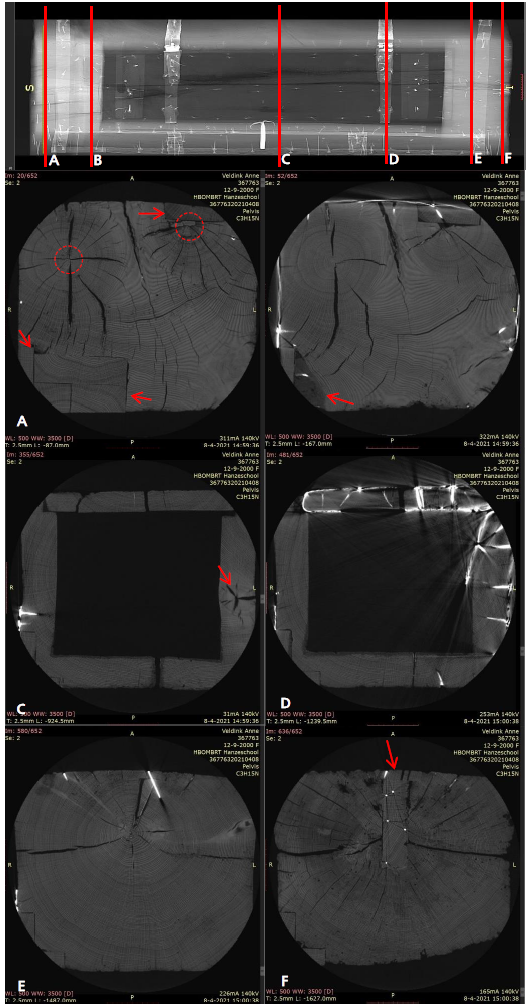
\includegraphics[width=0.9\textwidth,height=\textheight]{./figures/Doeve.png}

\hypertarget{s7-p-002}{%
\section*{S7-P-002}\label{s7-p-002}}
\addcontentsline{toc}{section}{S7-P-002}

\textbf{Out of the woods phase II}

Stephan Nicolaij\textsuperscript{1,~2}, Jelte van der Laan\textsuperscript{1,~3}

\emph{\textsuperscript{1} WOODAN Foundation, Groningen, The Netherlands. \textsuperscript{2} Qursi Software, Groningen, the Netherlands. \textsuperscript{3} Cambium Botany, Kleine Huisjes, the Netherlands.}

\href{mailto:Stephan.nicolaij@woodan.org}{\nolinkurl{Stephan.nicolaij@woodan.org}}

Over the last decades universities, government institutions and commercial companies have collected a huge amount of information on archaeological wooden artefacts. This information is scattered however, and there is no clear overview of what we know about wood utilisation and its development through time within a larger region. As most publications are focused on specific sites or excavations, it is often hard to place artifacts in a broader context.

In 2018 the WOODAN Foundation started collecting data on wooden artefacts with the mission to function as a central platform to find, analyse and publish information on these artefacts.

Thanks to the Flanders Heritage Agency we are enabled to do a big synthetic research project in Flanders. Our goal is to collect all data that is published on wooden artifacts since the Malta agreements, in order to conduct additional research. Also, the WOODAN database will be further developed in order to add data and to expand the functionality of translating the data to (for a start) four different languages. In this way language barriers will no longer be an issue in wood research. Our end products of this project will be:

• A book with an overview of the wooden artifacts found in Flanders

• The publication of the many finds in the WOODAN database

\hypertarget{s7-p-003}{%
\section*{S7-P-003}\label{s7-p-003}}
\addcontentsline{toc}{section}{S7-P-003}

\textbf{Measuring curved surfaces using photogrammetry}

Sjoerd van Daalen\textsuperscript{1}, Maarten Sepers\textsuperscript{2,~3}

\emph{\textsuperscript{1} Van Daalen Dendrochronologie, Deventer, the Netherlands. \textsuperscript{2} Department BBT Archaeology, Saxion University of Applied Sciences, Deventer, the Netherlands. \textsuperscript{3} DDEA, Deventer, the Netherlands.}

\href{mailto:vandaalen@dendro.nl}{\nolinkurl{vandaalen@dendro.nl}}

Dendrochronology uses tree-ring patterns in wooden objects to determine the age of the wood. In order to obtain an undistorted tree-ring sequence a radius along a transversal surface is preferred. For objects where destructive sampling is possible, this is easily solved by cutting a cross-section or taking a core. More delicate items, such as panel paintings and furniture pieces, are commonly rectangular and provide a transversal section where the tree-rings can be recorded using non-destructive methods. However, in the case of oval shaped painting or sculptures where the base is not usable, it is impossible to find a transversal section. Although tree-rings can be measured along a curved surface, the recorded values will be more distorted as the curvature increases. This renders the outer most tree-ring unusable. While the relative pattern of smaller and wider tree-rings will be preserved, it can no longer be presumed to be an absolute measurement. It is unclear what the effect of the distorted tree-ring pattern will be on the statistical results, especially if the curvature is not uniform. An orthogonal projection of a 3D model of the object creates a distortion-free view of the tree-ring pattern as well as a digital archive of the source data. 3D tomography has been successfully applied for this purpose, but the required equipment is not easily accessible.

In this paper we explore the possibilities of a photogrammetric approach for several case studies as well as propose practical guidelines for the application of this method.

\hypertarget{s7-p-004}{%
\section*{S7-P-004}\label{s7-p-004}}
\addcontentsline{toc}{section}{S7-P-004}

\textbf{X-ray-CT as possibility to date archived samples from Hallstatt, Austria}

Elisabeth Wächter\textsuperscript{1}, Hans Reschreiter\textsuperscript{2}, Kerstin Kowarik\textsuperscript{2}, Michael Grabner\textsuperscript{1}

\emph{\textsuperscript{1} Institute of Wood Technology and Renewable Materials, University of Natural Resources and Life Sciences, Vienna, Austria. \textsuperscript{2} Department of Prehistory, Natural History Museum, Vienna, Austria.}

\href{mailto:Elisabeth.waechter@boku.ac.at}{\nolinkurl{Elisabeth.waechter@boku.ac.at}}

In Hallstatt countless wooden samples from Bronze age and Iron age (Hallstatt time) are excavated and analysed every year. This is not the case for the subsequent La Tène period. There is only one spot in a raised bog near Hallstatt so called ``Dammwiese'' (1350 m a.s.l.) where numerous dwelling houses and a tunnel entrance from this period were examined in the 1880s and the first half of the 20th century. Nowadays these sites are not accessible anymore. Nevertheless, a few wood objects like parts of a log cabin, boards, the bottoms of barrels or buckets and fragments of shovels were excavated in former times and are well preserved available in the archive of the Natural History Museum Vienna. It was not desired to cut or drill holes in these unique finds. With the help of X-ray-CT-scans, it was possible to process these samples in a non-destructive way.

In total on 63 wooden elements from four different wood species (beech, spruce, larch and fir) tree-ring width measurements were carried out. Almost half of the measured samples could be synchronized and dated to the time from -263 to -123 resulting in three local mean curves (larch 89 years, fir 243 years and spruce 220 years).

To conclude, it can be worthwhile to take a close look at "old finds" in the archives and do the dendrochronological analyses in a usual way or non-destructively with the help of X-ray-CT-imaging.

\hypertarget{part-list-of-participants}{%
\part*{LIST OF PARTICIPANTS}\label{part-list-of-participants}}
\addcontentsline{toc}{part}{LIST OF PARTICIPANTS}

\hypertarget{list-of-participants}{%
\chapter*{List of participants}\label{list-of-participants}}
\addcontentsline{toc}{chapter}{List of participants}

\begin{itemize}
\tightlist
\item
  Aoife Daly
\item
  Marta Domínguez-Delmás
\item
  Kristof Haneca
\item
  \ldots{}
\end{itemize}

\end{document}
